\documentclass[12pt,a4paper]{article}

% ---------- Encoding & Fonts ----------
% NOTE: compile with XeLaTeX. Gurmukhi is Unicode and needs a system font;
% pdfLaTeX with inputenc/mathptmx cannot typeset it. Times New Roman keeps
% the Roman text identical to the synopsis.
\usepackage{fontspec}
\setmainfont{Times New Roman}
\newfontfamily\gur{Nirmala UI}[Script=Gurmukhi]
\usepackage{graphicx}
\usepackage{float}
\usepackage{tikz}
\usepackage{caption}
\captionsetup{font=it}
\captionsetup[table]{position=top}
\captionsetup[figure]{position=bottom}
\usepackage{listings}
\lstset{
  basicstyle=\ttfamily\small,
  inputencoding=utf8,
  extendedchars=true
}



% \usepackage{tocloft}

% \renewcommand{\cftsecleader}{\cftdotfill{\cftdotsep}}
% \renewcommand{\cftdotsep}{1}

\setcounter{tocdepth}{3}
\usetikzlibrary{shapes, arrows.meta, positioning, fit, calc}

% ---------- Page Geometry ----------
\usepackage[
  a4paper,
  top=2.5cm,
  bottom=1.25cm,
  left=3.5cm,
  right=1.25cm
]{geometry}
\setlength{\footskip}{0.8cm}

% ---------- Line Spacing ----------
\usepackage{setspace}
\onehalfspacing

% ---------- Text Alignment ----------
\usepackage{ragged2e}
\justifying

% ---------- Hyperlinks ----------
\usepackage[hidelinks]{hyperref}
\Urlmuskip=0mu plus 1mu
\renewcommand{\UrlFont}{\rmfamily}

% ---------- Lists ----------
\usepackage{enumitem}

% ---------- Section Formatting ----------
\usepackage{titlesec}
\titleformat{\section}
{\normalfont\Large\bfseries}
{\thesection.}
{1em}
{}
\titleformat{\subsection}{\normalfont\large\bfseries}{\thesubsection}{1em}{}
\titlespacing*{\section}{0pt}{12pt}{6pt}
\titlespacing*{\subsection}{0pt}{10pt}{5pt}

% ---------- Paragraph Formatting ----------
\setlength{\parindent}{1.27cm}
\setlength{\parskip}{0pt}


\usepackage[numbers,sort&compress]{natbib}

% ---------- Tables ----------
\usepackage{longtable}
\usepackage{array}



\begin{document}

% ===================== TITLE PAGE =====================
\begin{titlepage}
\begin{center}

% --- Top label ---
{\fontsize{16}{16}\selectfont \textbf{A Midterm Progress Report}}\\[0.4cm]
{\fontsize{14}{14}\selectfont on}\\[0.6cm]

% --- Project Title (24pt, uppercase, bold) ---

{\fontsize{24}{24}\selectfont \textbf{ Semantic Retrieval and\\[0.2cm]Contextual Exploration System}}\\[0.8cm]


% --- Report Type ---
{\fontsize{12}{14}\selectfont \textbf{Submitted in partial fulfillment of the requirements for the award of}}\\[0.1cm]
{\fontsize{12}{14}\selectfont \textbf{the degree of}}\\[0.8cm]

% --- Degree ---
{\fontsize{14}{12}\large \textbf{BACHELOR OF TECHNOLOGY}}\\
{\fontsize{16}{12}\large (Computer Science and Engineering)}


\end{center}
% --- Submitted By ---
\vspace{1cm}

\begin{center}
    {\fontsize{14}{14}\selectfont SUBMITTED BY:}\\[0.4cm]

    {\fontsize{14}{14}\selectfont Balkaran Singh \quad (2302494)}\\
    {\fontsize{14}{14}\selectfont Gurpreet Kaur \quad (2302530)}\\
    {\fontsize{14}{10}\selectfont Gurveer Singh \quad (2302533)}\\[0.8cm]

    {\fontsize{14}{14}\selectfont UNDER THE GUIDANCE OF}\\[0.3cm]
    {\fontsize{14}{14}\selectfont \textbf{Dr. Parminder Singh}}\\[0.5cm]
    {\fontsize{12}{12}\selectfont (October 2026)}
\end{center}

\vfill

% --- College Logo ---
\begin{center}
    
\includegraphics[height=5.5cm]{logo-70-Edited.png}
\end{center}

\vfill

% --- Department ---
\begin{center}

    {\large\textbf{Department of Computer Science and Engineering}}\\
    {\large\textbf{GURU NANAK DEV ENGINEERING COLLEGE}}\\
    {\large\textbf{LUDHIANA, 141006}}\\[0.3cm]

\end{center}

\end{titlepage}
% ===================== END TITLE PAGE =====================

% ===================== TABLE OF CONTENTS =====================

\newpage
\clearpage
\pagenumbering{roman}

\begin{center}
\textbf{\Large Table of Contents}
\end{center}
\addcontentsline{toc}{section}{Table of Contents}

\begin{table}[H]
\centering
\renewcommand{\arraystretch}{1.4}

\begin{tabular}{|p{11cm}|c|}
\hline
\textbf{Contents} & \textbf{Page No.} \\
\hline
1. Introduction & 1 \\
\hline
2. System Requirements & 4 \\
\hline
3. Software Requirement Analysis & 6 \\
\hline
4. Software Design & 9 \\
\hline
5. Testing Module & 19 \\
\hline
6. Performance of the Project Developed & 22 \\
\hline
7. Output Screens & 31 \\
\hline
8. References & 34 \\
\hline
\end{tabular}
\end{table}

% ===================== LIST OF FIGURES =====================
\newpage
\begin{center}
\textbf{\Large List of Figures}
\end{center}
\addcontentsline{toc}{section}{List of Figures}
\listoffigures



% ===================== INTRODUCTION =====================
\clearpage
\pagenumbering{arabic}
\setcounter{page}{1}
\newpage
\section{Introduction}

Semantic understanding is an important area of Natural Language Processing (NLP) that focuses on identifying the meaning and intent conveyed by a piece of text rather than simply matching individual words. Traditional text retrieval techniques often depend on keywords, exact matching, or surface-level lexical similarity, which can fail when two texts express the same idea using different vocabulary or sentence structures. Context understanding addresses this limitation by considering the relationship between words and the overall meaning of a sentence or passage. Recent advances in deep learning and language representation models have enabled text to be represented as contextual embeddings, where semantically similar texts can be positioned close to each other in a shared vector space \cite{feng2022labse, wang2024multilinguale5}.

This problem of contextual and semantic understanding becomes particularly significant when working with Gurbani. Sri Guru Granth Sahib contains a vast collection of Gurbani written in Gurmukhi, where the meaning of a Pankati (line) is often dependent not only on individual words but also on the overall spiritual and contextual message conveyed by it. A literal word-level interpretation may therefore be insufficient for identifying other Pankatis that express a similar teaching or spiritual idea. The project addresses this limitation by developing an AI-based system capable of understanding the contextual meaning, or \textit{Bhavarth}, of a Gurbani Pankati and retrieving other Pankatis that convey a similar spiritual or contextual idea.

The central difficulty is that the same teaching may be expressed in entirely different vocabulary. For example, the Pankati \textit{``\gur{ਵਿਸਰੀ ਤਿਸੈ ਪਰਾਈ ਤਾਤਾ}''} (Ang 189) and the Pankati \textit{``\gur{ਛਾਡਿ ਵਿਡਾਣੀ ਤਾਤਿ ਮੂੜੇ}''} (Ang 889) both teach the abandonment of envy towards others, yet they share no common word and are separated by seven hundred Angs. No keyword-based search system can connect them. A system that understands meaning, however, should place them close together.

\subsection{Work Completed in This Phase}

During the current phase of the project, the following work has been completed. A structured Gurbani dataset of 60,360 Pankatis with five independent commentaries (Steeks) was profiled and cleaned. A leakage-free training and evaluation split was constructed. An automatic evaluation benchmark of 827 verse-to-verse queries was mined from the commentaries. A baseline was established using the pretrained BGE-M3 embedding model and two keyword-search baselines. The embedding model was then fine-tuned on Gurbani-specific training pairs using Low-Rank Adaptation (LoRA) \cite{hu2022lora}, and the improvement was measured against the same benchmark.
\newpage

\subsection{Objectives}

Following are the objectives for the project work:

\begin{enumerate}
    \item To develop a semantic representation framework for capturing the contextual meaning (\textit{Bhavarth}) of Gurbani text.

    \item To develop a semantic retrieval system for identifying and ranking Gurbani Pankatis based on contextual and thematic similarity.

    \item To develop an intelligent Gurbani information system integrating semantic retrieval with Gurbani metadata, Raag information, and relevant digital resources.
\end{enumerate}
\newpage
\subsection{Elaboration of the Objectives}

\noindent\textbf{Objective 1: Semantic representation framework.}
This objective requires that a Gurbani Pankati be converted into a numerical representation that encodes its meaning rather than its spelling. A pretrained multilingual embedding model \cite{chen2024bgem3} cannot do this on its own, because it has never been exposed to Gurbani. The objective is therefore met by adapting such a model using supervision derived from the Steeks written by traditional commentators. Each Pankati is aligned with the explanations given for it, so that verses explained in similar terms acquire similar representations.

\vspace{0.3cm}

\noindent\textbf{Objective 2: Semantic retrieval and ranking.}
Once every Pankati is represented as a vector, retrieval becomes a nearest-neighbour search in the vector space \cite{karpukhin2020dpr, douze2024faiss}. This objective requires that the ranking produced by the system be measurably better than keyword search. To establish this, an evaluation benchmark and two keyword baselines were constructed, and all systems were scored on identical queries.

\vspace{0.3cm}

\noindent\textbf{Objective 3: Intelligent Gurbani information system.}
Retrieved Pankatis are of limited use without context. This objective requires that each result be presented with its Ang number, Raag, Shabad identifier, and the Steeks that explain it, and that results be drawn from different Shabads so that the user discovers Gurbani beyond the passage already in front of them.


% ===================== END INTRODUCTION =====================

% ===================== SYSTEM REQUIREMENTS =====================
\newpage
\section{System Requirements}
\addcontentsline{toc}{section}{System Requirements}

The project has two distinct computational phases with different requirements. Data preparation, retrieval, and evaluation are light enough for a standard laptop, whereas fine-tuning a 568-million-parameter transformer model requires a CUDA-capable graphics processor. Both configurations are described below, since both were used during development.

\subsection{Hardware Requirements}

\begin{center}
\renewcommand{\arraystretch}{1.35}

\begin{table}[htbp]
\centering
\caption{Hardware requirements}
\label{tab:hardware}
\begin{tabular}{|p{3.6cm}|p{5.2cm}|p{5.2cm}|}
\hline
\textbf{Component} & \textbf{Development Machine} & \textbf{Training Machine} \\
\hline
Processor & Intel Core i3-1005G1, 2 cores / 4 threads, 1.20 GHz & Multi-core desktop processor \\
\hline
Memory (RAM) & 11.8 GB & 16 GB \\
\hline
Graphics & Intel UHD Graphics (integrated, no CUDA) & NVIDIA GeForce RTX 3060, 12 GB VRAM \\
\hline
Storage & 5 GB free space for datasets, embeddings and model files & 10 GB free space \\
\hline
Connectivity & Stable internet for downloading pretrained models & Stable internet \\
\hline
\end{tabular}
\end{table}
\end{center}

\vspace{0.3cm}

The distinction between the two machines is not incidental. Fine-tuning BGE-M3 with the Adam optimiser requires approximately sixteen bytes per parameter for the weights, their gradients and the optimiser state, which amounts to roughly nine gigabytes before any activations are stored. This does not fit comfortably within the memory available on the development laptop, and in the absence of a CUDA device every operation would execute on two low-clock CPU cores. The measured cost of a single forward pass over the corpus on the development machine was 112 minutes; a training run, which requires both forward and backward passes over a far larger number of samples, would therefore be impractical. Training was consequently performed on the RTX 3060, where the same work completes in minutes.

\subsection{Software Requirements}

\begin{table}[H]
\centering
\renewcommand{\arraystretch}{1.35}
\caption{Software requirements}
\begin{tabular}{|p{4.6cm}|p{3.0cm}|p{6.2cm}|}
\hline
\textbf{Software} & \textbf{Version} & \textbf{Purpose} \\
\hline
Windows & 10 / 11 & Operating system \\
\hline
Python & 3.11 & Implementation language \\
\hline
PyTorch & 2.14 (CPU and CUDA builds) & Deep learning framework \\
\hline
Sentence-Transformers & 6.0.1 & Embedding model training and inference \\
\hline
Transformers & 5.16.1 & Underlying model architecture \\
\hline
PEFT & 0.21.0 & Low-Rank Adaptation (LoRA) \\
\hline
FAISS & 1.15.0 & Vector similarity search \\
\hline
scikit-learn & 1.9.0 & TF--IDF based pair mining \\
\hline
pandas / NumPy & 3.0.5 / 2.4.6 & Data processing \\
\hline
rank\_bm25 & 0.2.2 & Keyword-search baseline \\
\hline
openpyxl & 3.1.5 & Reading the source workbook \\
\hline
python-dotenv & 1.2.3 & Configuration management \\
\hline
Visual Studio Code & Latest & Development environment \\
\hline
Git & Latest & Version control \\
\hline
\end{tabular}
\end{table}

\subsection{Pretrained Model Requirement}

The system uses \textbf{BGE-M3} (\texttt{BAAI/bge-m3}) \cite{chen2024bgem3} as the base embedding model. It is a multilingual text-embedding model built on the XLM-RoBERTa-large architecture, containing 568 million parameters arranged in 24 transformer layers, and producing embeddings of 1024 dimensions. The model is approximately 2.3 GB in size and is downloaded once from the Hugging Face model repository. It was selected because it supports more than one hundred languages including Punjabi, handles long input sequences, and is designed specifically for retrieval rather than classification.

\subsection{Dependency Management}

Because the project is developed across machines with and without a CUDA device, the dependency specification is split into three files. A shared file lists the version-independent packages; a CPU file adds the CPU build of PyTorch; and a GPU file adds the CUDA build together with the additional packages required for training. A single requirements file cannot serve both configurations, since installing the CUDA build on a machine without an NVIDIA device wastes approximately 2.5 GB, while installing the CPU build on the training machine would make the graphics processor unusable.

% ===================== END SYSTEM REQUIREMENTS =====================

% ===================== SOFTWARE REQUIREMENT ANALYSIS =====================
\newpage
\section{Software Requirement Analysis}
\addcontentsline{toc}{section}{Software Requirement Analysis}

\subsection{Problem Definition}

Given a Gurbani Pankati as input, the system must return other Pankatis from Sri Guru Granth Sahib that convey the same contextual meaning (\textit{Bhavarth}), together with their metadata and commentaries. The returned Pankatis must be ranked by semantic relevance, and the ranking must remain correct when the related Pankatis share no vocabulary with the input.

The problem has three properties that make it difficult:

\begin{enumerate}[leftmargin=*, label=(\alph*), itemsep=0.2cm]
    \item \textbf{Absence of ground truth.} There exists no labelled dataset stating that one Pankati is semantically similar to another. Supervision must therefore be derived from an indirect source.

    \item \textbf{Vocabulary mismatch.} Measurements on the prepared corpus show that among Pankatis judged semantically related, a substantial proportion share no words at all. Lexical retrieval cannot reach these cases even in principle.

    \item \textbf{Absence of a Gurbani-aware model.} General-purpose multilingual models \cite{kakwani2020indicnlpsuite, ramesh2022samanantar, deode2023indicsbert} are trained on contemporary web text. They have no exposure to the archaic Gurmukhi of Sri Guru Granth Sahib and consequently fall back on surface-level similarity.
\end{enumerate}

\subsection{Key Insight Underlying the Solution}

The problem of missing ground truth is solved by observing that the semantic work has already been performed by traditional scholars. The dataset contains, for each Pankati, explanations written in modern Punjabi prose by several independent commentators. Two Pankatis that mean the same thing are explained in very similar words, even when the Pankatis themselves share no vocabulary. The following example illustrates this:

\begin{table}[H]
\centering
\renewcommand{\arraystretch}{1.3}
\caption{The semantic problem is difficult on the verses and easy on the commentaries}
\begin{tabular}{|p{2.6cm}|p{10.5cm}|}
\hline
\textbf{Pankati A} & \gur{ਵਿਸਰੀ ਤਿਸੈ ਪਰਾਈ ਤਾਤਾ} \\
\hline
\textbf{Pankati B} & \gur{ਛਾਡਿ ਵਿਡਾਣੀ ਤਾਤਿ ਮੂੜੇ} \\
\hline
\textbf{Shared words} & none \\
\hline
\textbf{Steek of A} & \gur{ਉਸ ਨੂੰ ਹੋਰਨਾਂ ਨਾਲ ਈਰਖਾ ਕਰਨੀ ਭੁੱਲ ਜਾਂਦੀ ਹੈ} \\
\hline
\textbf{Steek of B} & \gur{ਹੇ ਮੂਰਖ}! \gur{ਦੂਜਿਆਂ ਨਾਲ ਈਰਖਾ ਕਰਨੀ ਛੱਡ ਦੇ} \\
\hline
\textbf{Shared words} & \gur{ਈਰਖਾ}, \gur{ਕਰਨੀ}, \gur{ਨਾਲ} \\
\hline
\end{tabular}
\end{table}

\vspace{0.3cm}

The semantic relationship that is invisible at the level of the verses becomes a simple word-overlap count at the level of the commentaries. This observation is used twice in the system: to generate training supervision, and to generate an evaluation benchmark.

\subsection{Functional Requirements}

\begin{table}[H]
\centering
\renewcommand{\arraystretch}{1.3}
\caption{Functional requirements}
\begin{tabular}{|c|p{11.2cm}|}
\hline
\textbf{ID} & \textbf{Requirement} \\
\hline
FR-1 & The system shall accept a Gurbani Pankati as input, with or without the terminating danda and verse numbers. \\
\hline
FR-2 & The system shall accept multiple Pankatis, or a complete Shabad, as a single query. \\
\hline
FR-3 & The system shall return the top $k$ semantically related Pankatis, ranked by similarity. \\
\hline
FR-4 & The system shall exclude Pankatis belonging to the same Shabad as the query. \\
\hline
FR-5 & The system shall return at most one Pankati per Shabad, so that results are diverse. \\
\hline
FR-6 & The system shall display the Ang number, Raag, Shabad identifier and Steek for every retrieved Pankati. \\
\hline
FR-7 & The system shall support comparison between two models in a single run. \\
\hline
FR-8 & The system shall exclude structural heading lines from the searchable corpus. \\
\hline
FR-9 & The system shall treat a Pankati that repeats in the scripture as one searchable entry. \\
\hline
\end{tabular}
\end{table}

\subsection{Non-Functional Requirements}

\begin{table}[H]
\centering
\renewcommand{\arraystretch}{1.3}
\caption{Non-functional requirements}
\begin{tabular}{|c|p{11.2cm}|}
\hline
\textbf{ID} & \textbf{Requirement} \\
\hline
NFR-1 & A query against a Pankati already present in the corpus shall be answered without loading the embedding model. \\
\hline
NFR-2 & Corpus embedding shall be resumable, so that an interrupted run does not restart. \\
\hline
NFR-3 & All file paths and hyper-parameters shall be configurable without modifying source code. \\
\hline
NFR-4 & Training runs shall be reproducible through fixed random seeds. \\
\hline
NFR-5 & The source dataset shall never be modified; every stage shall write new files. \\
\hline
NFR-6 & Evaluation shall be free of data leakage between training and test partitions. \\
\hline
\end{tabular}
\end{table}

\subsection{Modules and Their Functionalities}

The system is decomposed into six modules. Each module is implemented as an independent script that reads the output of the previous stage and writes new files, so that any stage can be re-executed without repeating the others.

\vspace{0.3cm}

\noindent\textbf{Module 1 --- Data Preprocessing (\texttt{clean\_dataset.py}).}
Reads the source workbook, normalises whitespace and removes markup, identifies structural heading lines, detects Pankatis that repeat within the scripture, counts the commentaries available for each Pankati, and writes a cleaned dataset together with a profile report and an audit file of every excluded row. The original workbook is opened read-only.

\vspace{0.3cm}

\noindent\textbf{Module 2 --- Training Pair Construction (\texttt{create\_training\_pairs.py}).}
Partitions the cleaned dataset into training, validation and test sets using a grouping procedure that prevents leakage, generates Pankati--Steek training pairs, and writes the deduplicated retrieval corpus with its metadata and commentaries attached.

\vspace{0.3cm}

\noindent\textbf{Module 3 --- Benchmark Construction (\texttt{build\_eval\_sets.py}).}
Mines an evaluation benchmark of verse-to-verse queries from the test partition by identifying Pankati pairs that two independent commentators explain in similar terms.

\vspace{0.3cm}

\noindent\textbf{Module 4 --- Training Data Mining (\texttt{mine\_verse\_pairs.py}, \texttt{mine\_hard\_negatives.py}).}
Mines Pankati-to-Pankati positive pairs from the training partition using the same two-commentator rule, and then mines hard negatives, that is, Pankatis which share substantial vocabulary with the anchor but are explained differently.

\vspace{0.3cm}

\noindent\textbf{Module 5 --- Model Training (\texttt{train\_bge.py}).}
Fine-tunes BGE-M3 on the mined pairs using Low-Rank Adaptation \cite{hu2022lora} and a contrastive objective, verifies that the trained model differs behaviourally from the base model, and saves the adapter.

\vspace{0.3cm}

\noindent\textbf{Module 6 --- Retrieval and Evaluation (\texttt{build\_index.py}, \texttt{semantic\_search.py}, \texttt{evaluate.py}, \texttt{diagnose\_transfer.py}).}
Encodes the corpus into vectors, performs interactive retrieval with diversification and metadata display, and scores any number of retrieval systems on the benchmark.

% ===================== END SOFTWARE REQUIREMENT ANALYSIS =====================

% ===================== SOFTWARE DESIGN =====================
\newpage
\section{Software Design}
\addcontentsline{toc}{section}{Software Design}

This chapter presents the detailed design of the system. It begins with the overall architecture, then describes the design of each stage of the pipeline, and finally presents the standard design diagrams required for the solution of the three objectives listed in Chapter 1.

\subsection{System Architecture}

The system is organised as an offline preparation pipeline and an online retrieval path. The offline pipeline cleans the dataset, constructs training data, trains the embedding model and encodes the corpus into a vector index. The online path accepts a query, embeds it, searches the index, applies diversification and presents the results with their metadata. The architecture is shown in Figure~\ref{fig:architecture}.

\begin{figure}[htbp]


\centering

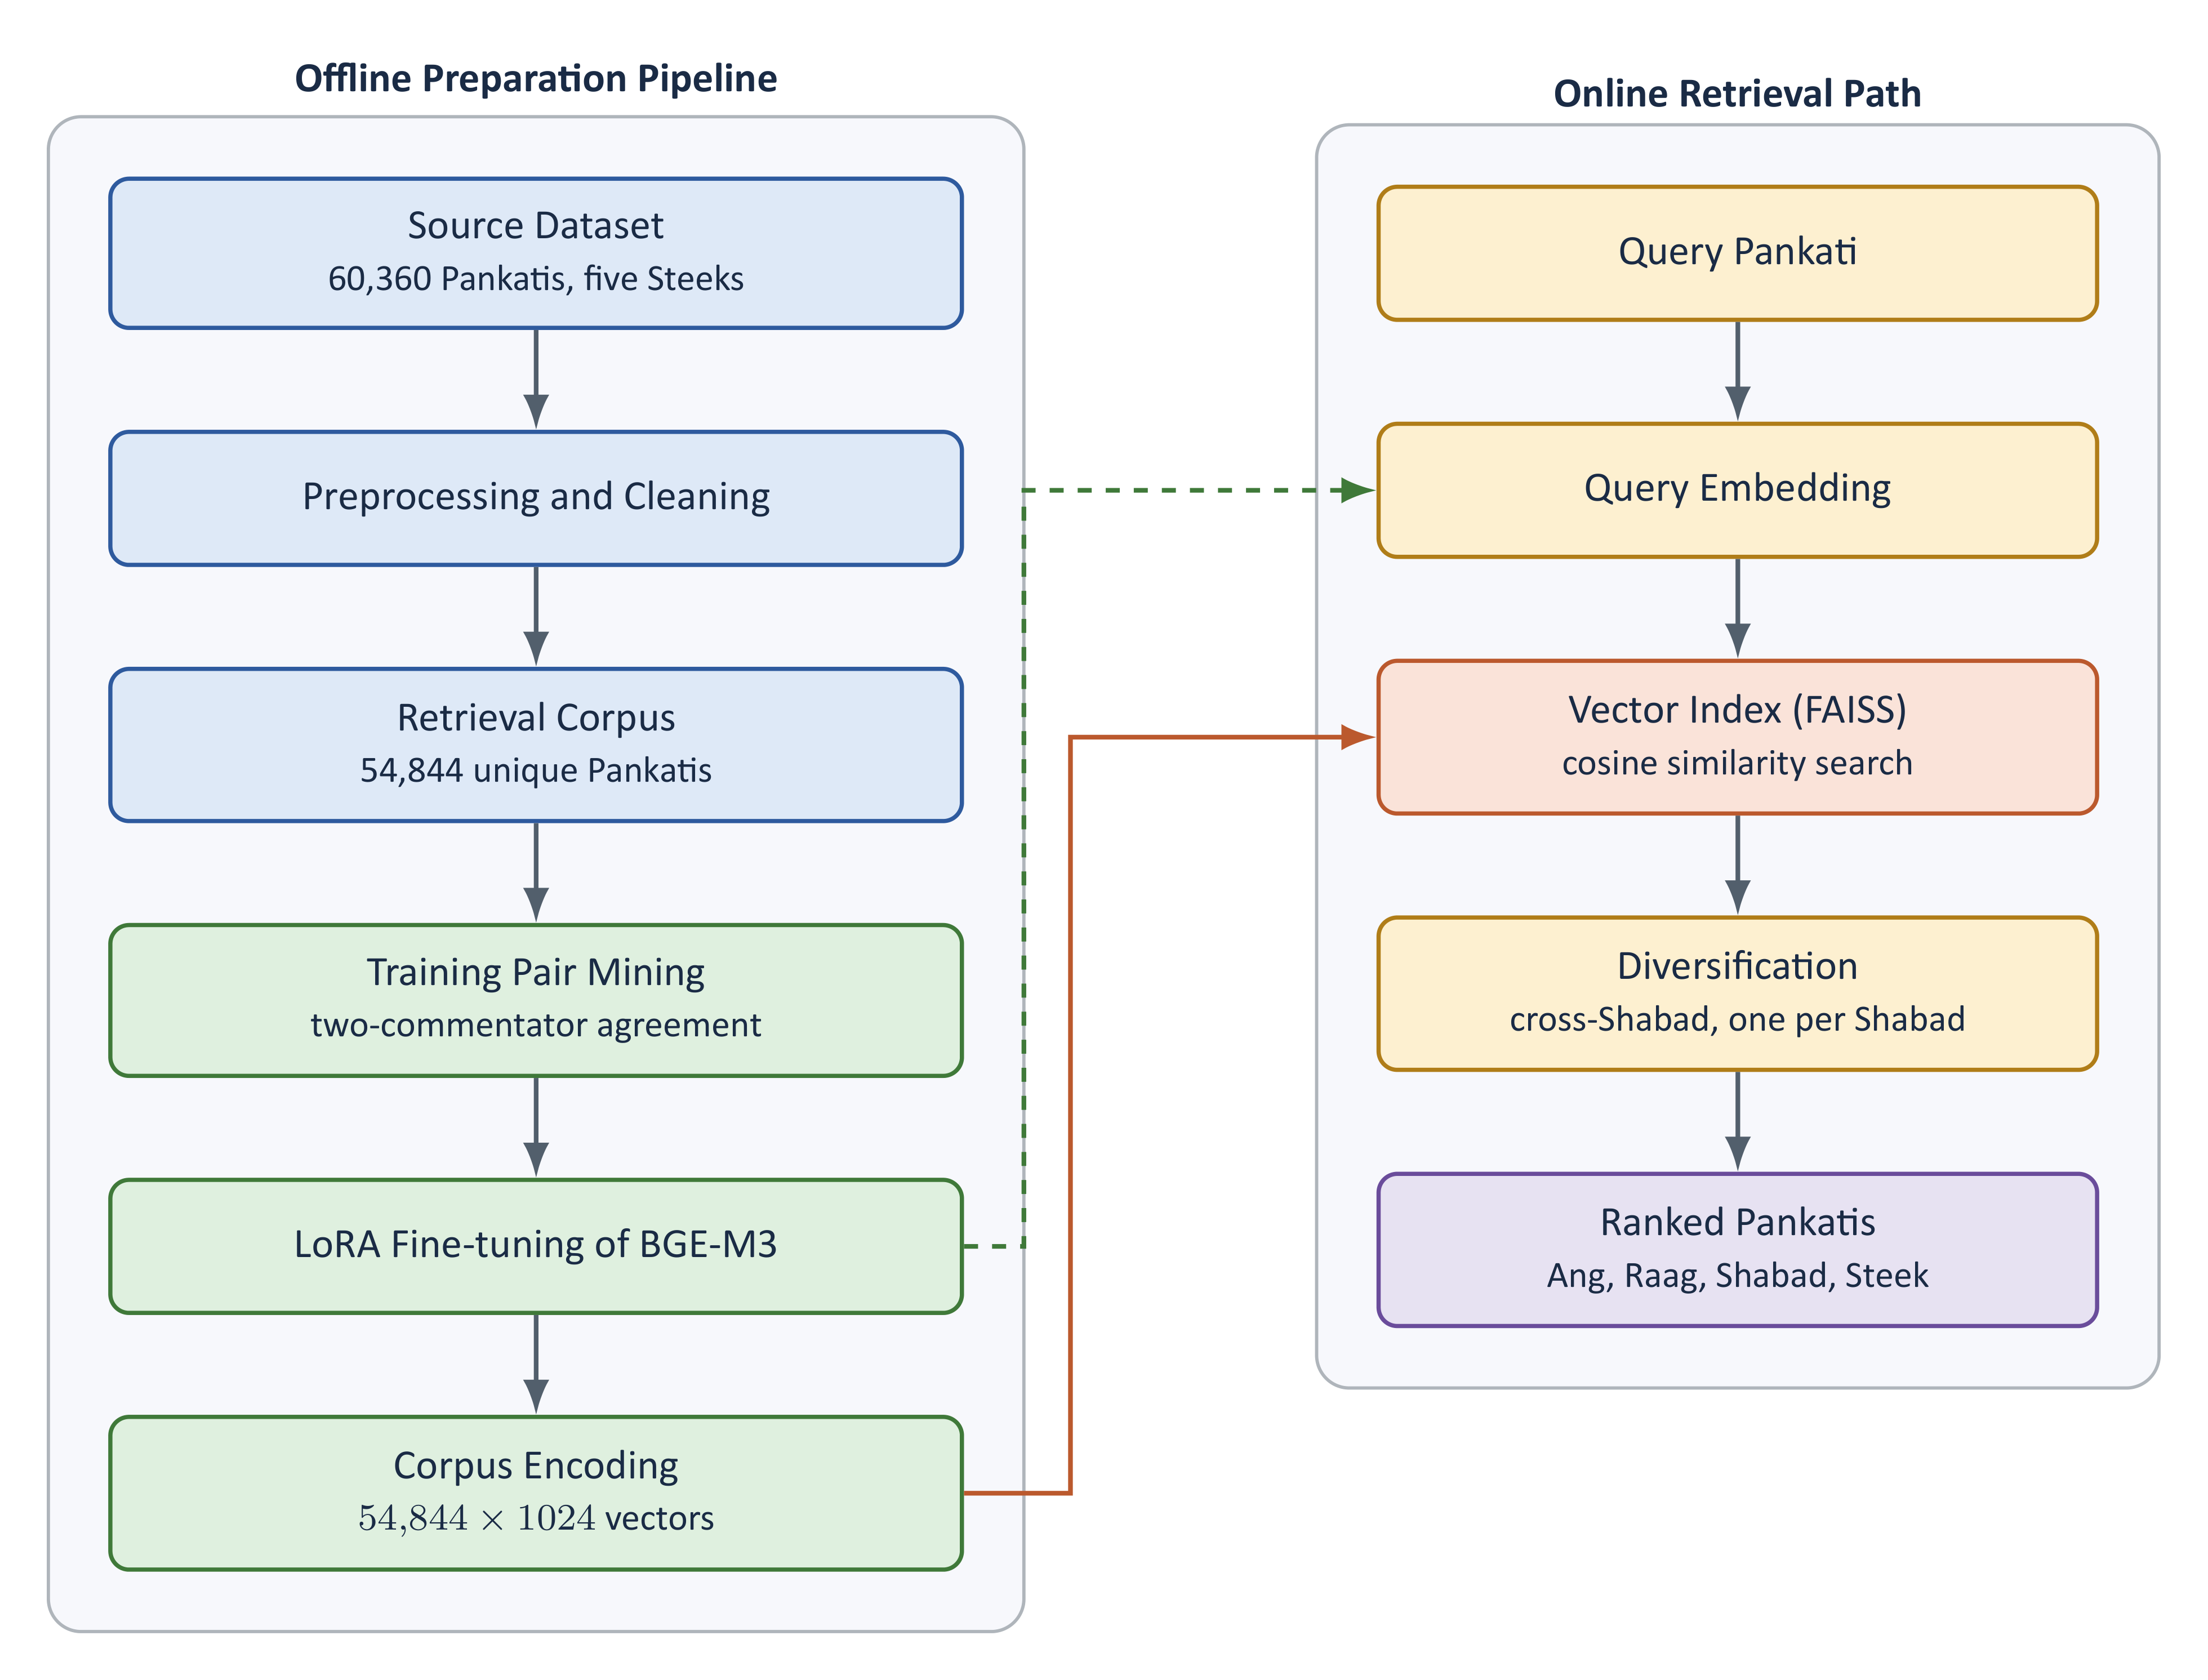
\includegraphics[width=\textwidth]{fig_diag_architecture.png}

\caption{System architecture of the Gurbani semantic retrieval system}
\label{fig:architecture}

\end{figure}

\subsection{Design of the Data Preprocessing Stage}

The preprocessing stage has to solve a problem that is not visible in the raw data. The source workbook contains a flag marking structural lines, but this flag identifies only 720 rows, whereas the corpus contains approximately five thousand such lines. Headings such as \textit{``\gur{ੴ ਸਤਿਗੁਰ ਪ੍ਰਸਾਦਿ}''} occur 522 times and \textit{``\gur{ਪਉੜੀ}''} occurs 515 times. These are section titles rather than teachings, and because they repeat verbatim they would also disturb contrastive training.

Two complementary detectors are therefore applied. The first matches prefix patterns characteristic of headings. The second matches a vocabulary rule: a short line terminated by a danda whose every token is a raag name or a composition term is a heading, not a teaching. The raag vocabulary is derived from the project's own raag metadata file and compared on consonant skeletons so that spelling variants such as \textit{\gur{ਬਿਲਾਵਲੁ}} and \textit{\gur{ਬਿਲਾਵਲ}} are unified.

A scripture guard protects genuine verses from both detectors: a line of thirty characters or more that all three commentators chose to translate is a teaching, irrespective of the word it begins with. This guard rescues verses such as \textit{``\gur{ਰਾਗੁ ਨਾਦੁ ਸਭੁ ਸਚੁ ਹੈ ਕੀਮਤਿ ਕਹੀ ਨ ਜਾਇ}''}, which would otherwise be removed by the raag-heading rule.


\begin{figure}[H]
\centering
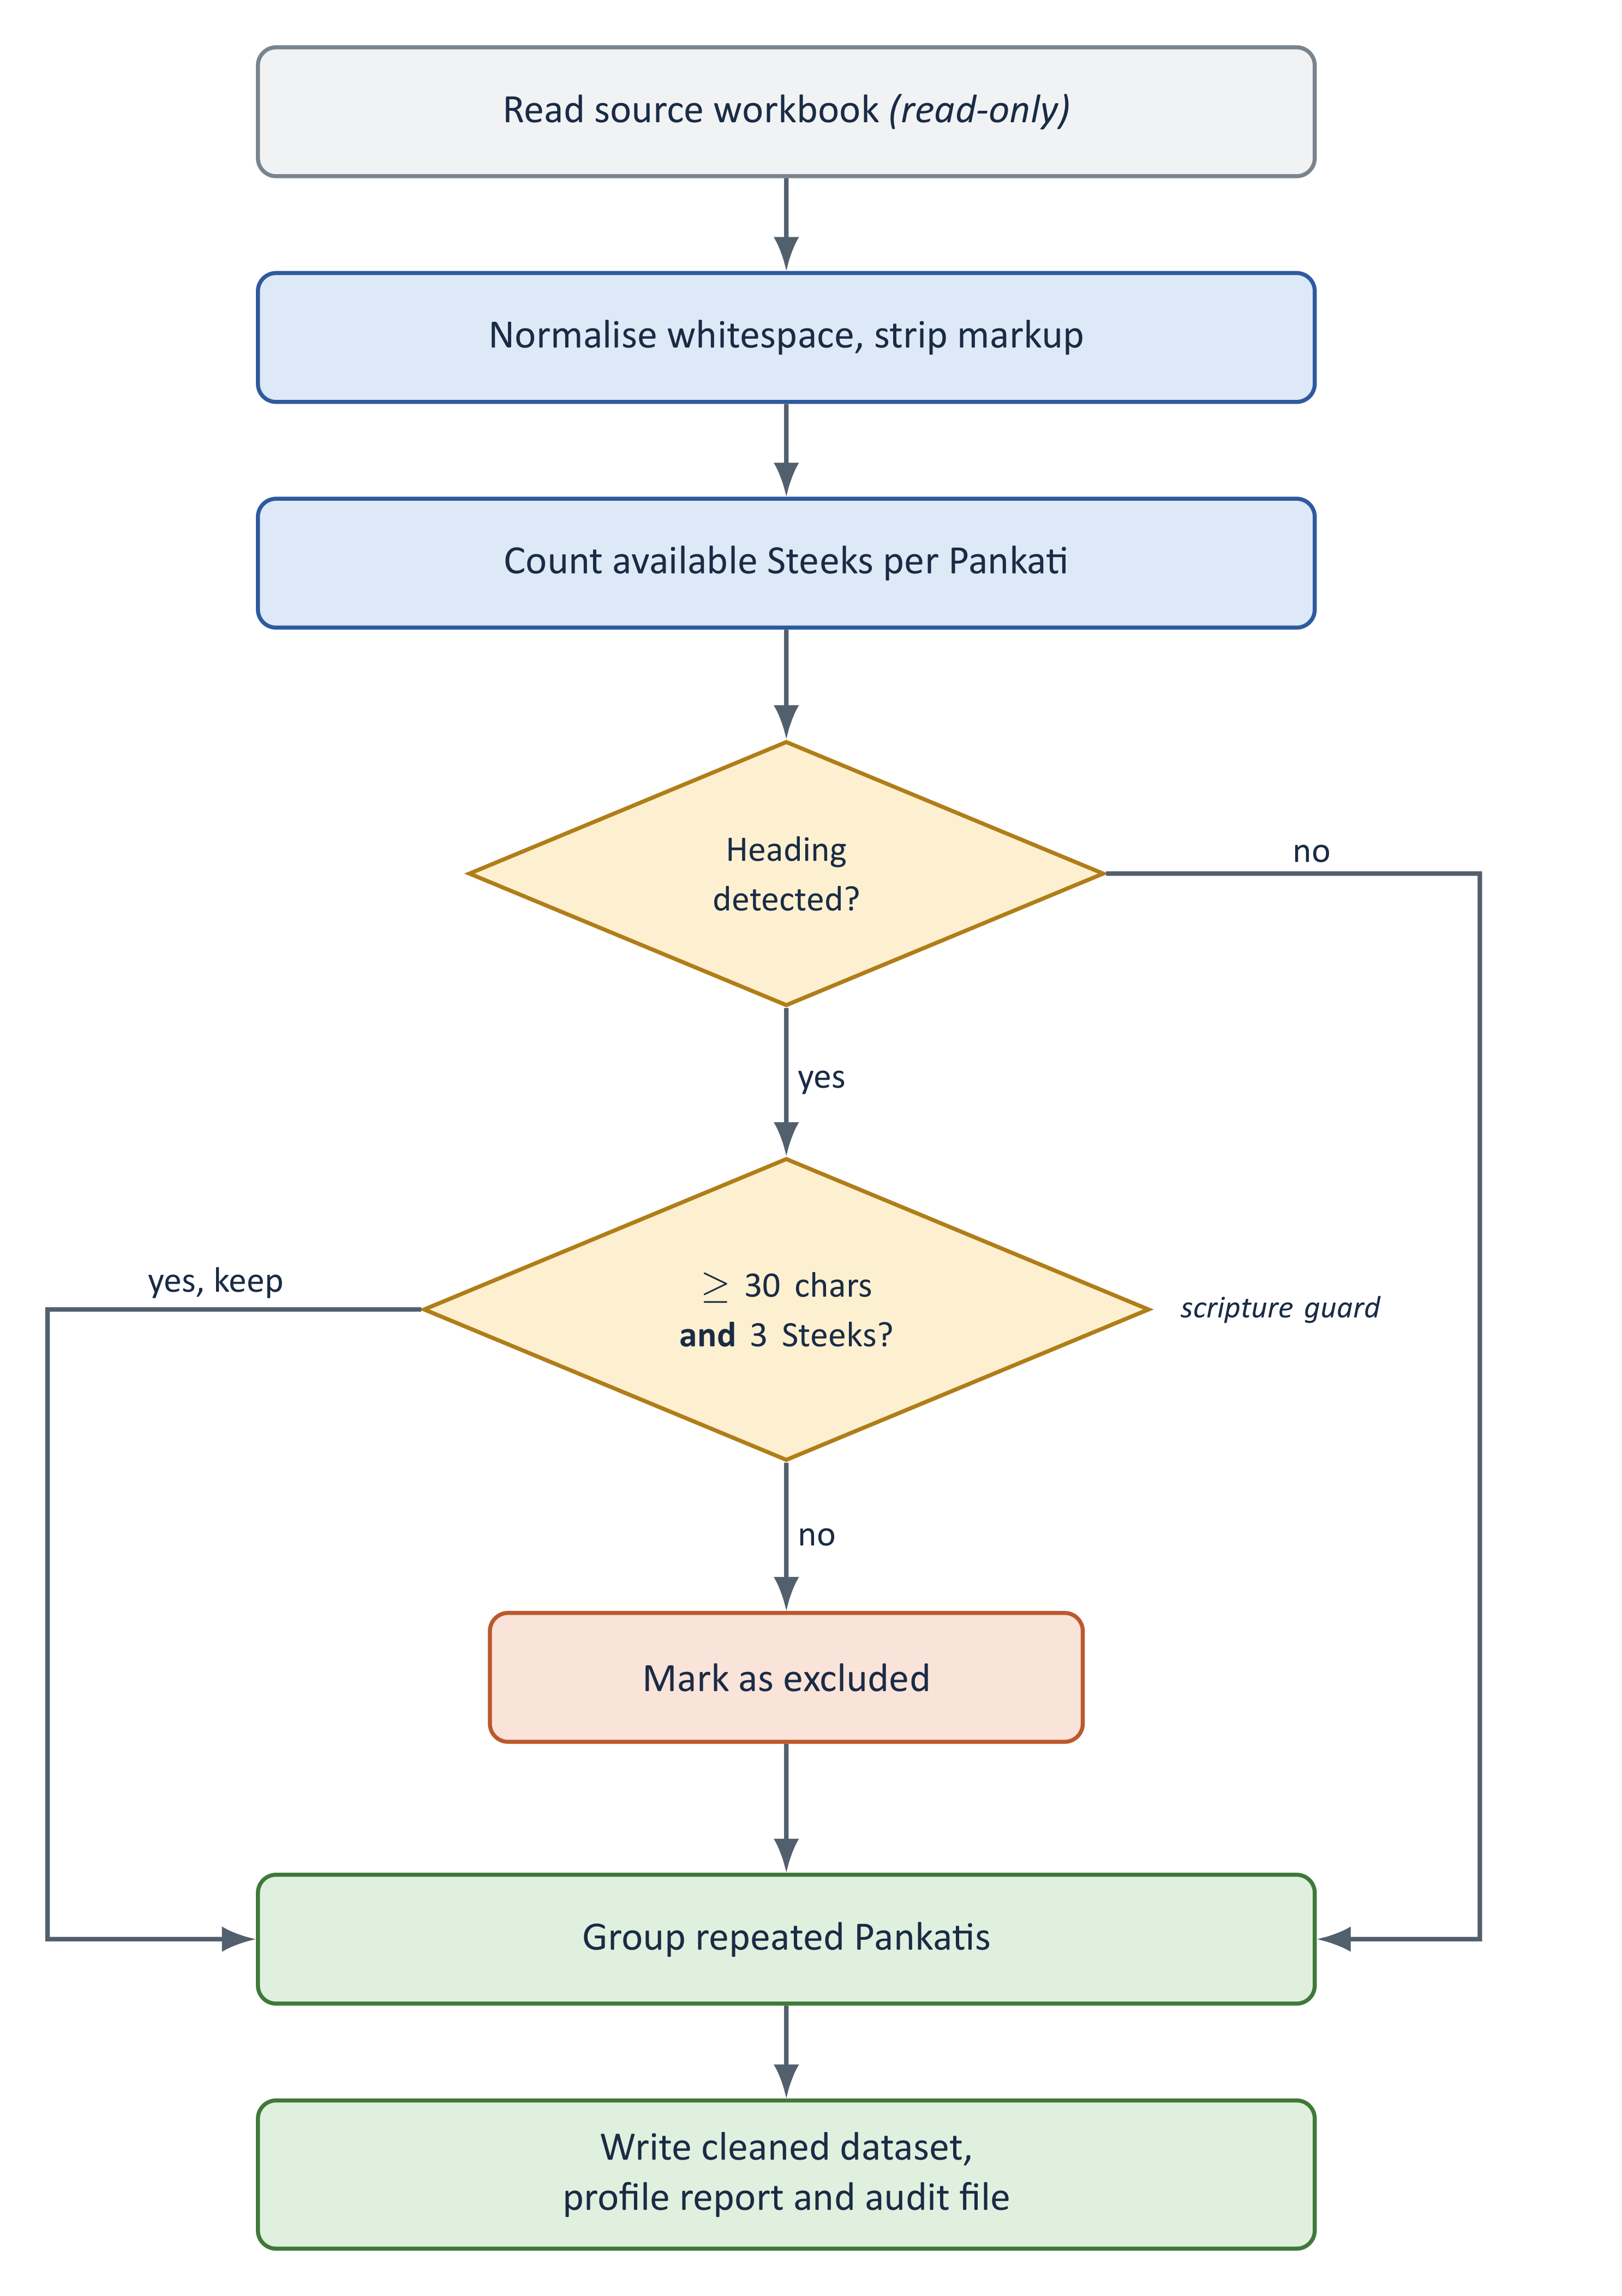
\includegraphics[width=0.82\textwidth]{fig_diag_preprocess.png}
\caption{Data preprocessing pipeline}
\label{fig:preprocess}
\end{figure}

\subsection{Data Flow Diagrams}

\subsubsection{Level 0 (Context Diagram)}

At the highest level the system accepts a Pankati from the user and returns semantically related Pankatis together with their associated information. The scripture dataset and the pretrained model act as external data sources.


\begin{figure}[H]
\centering
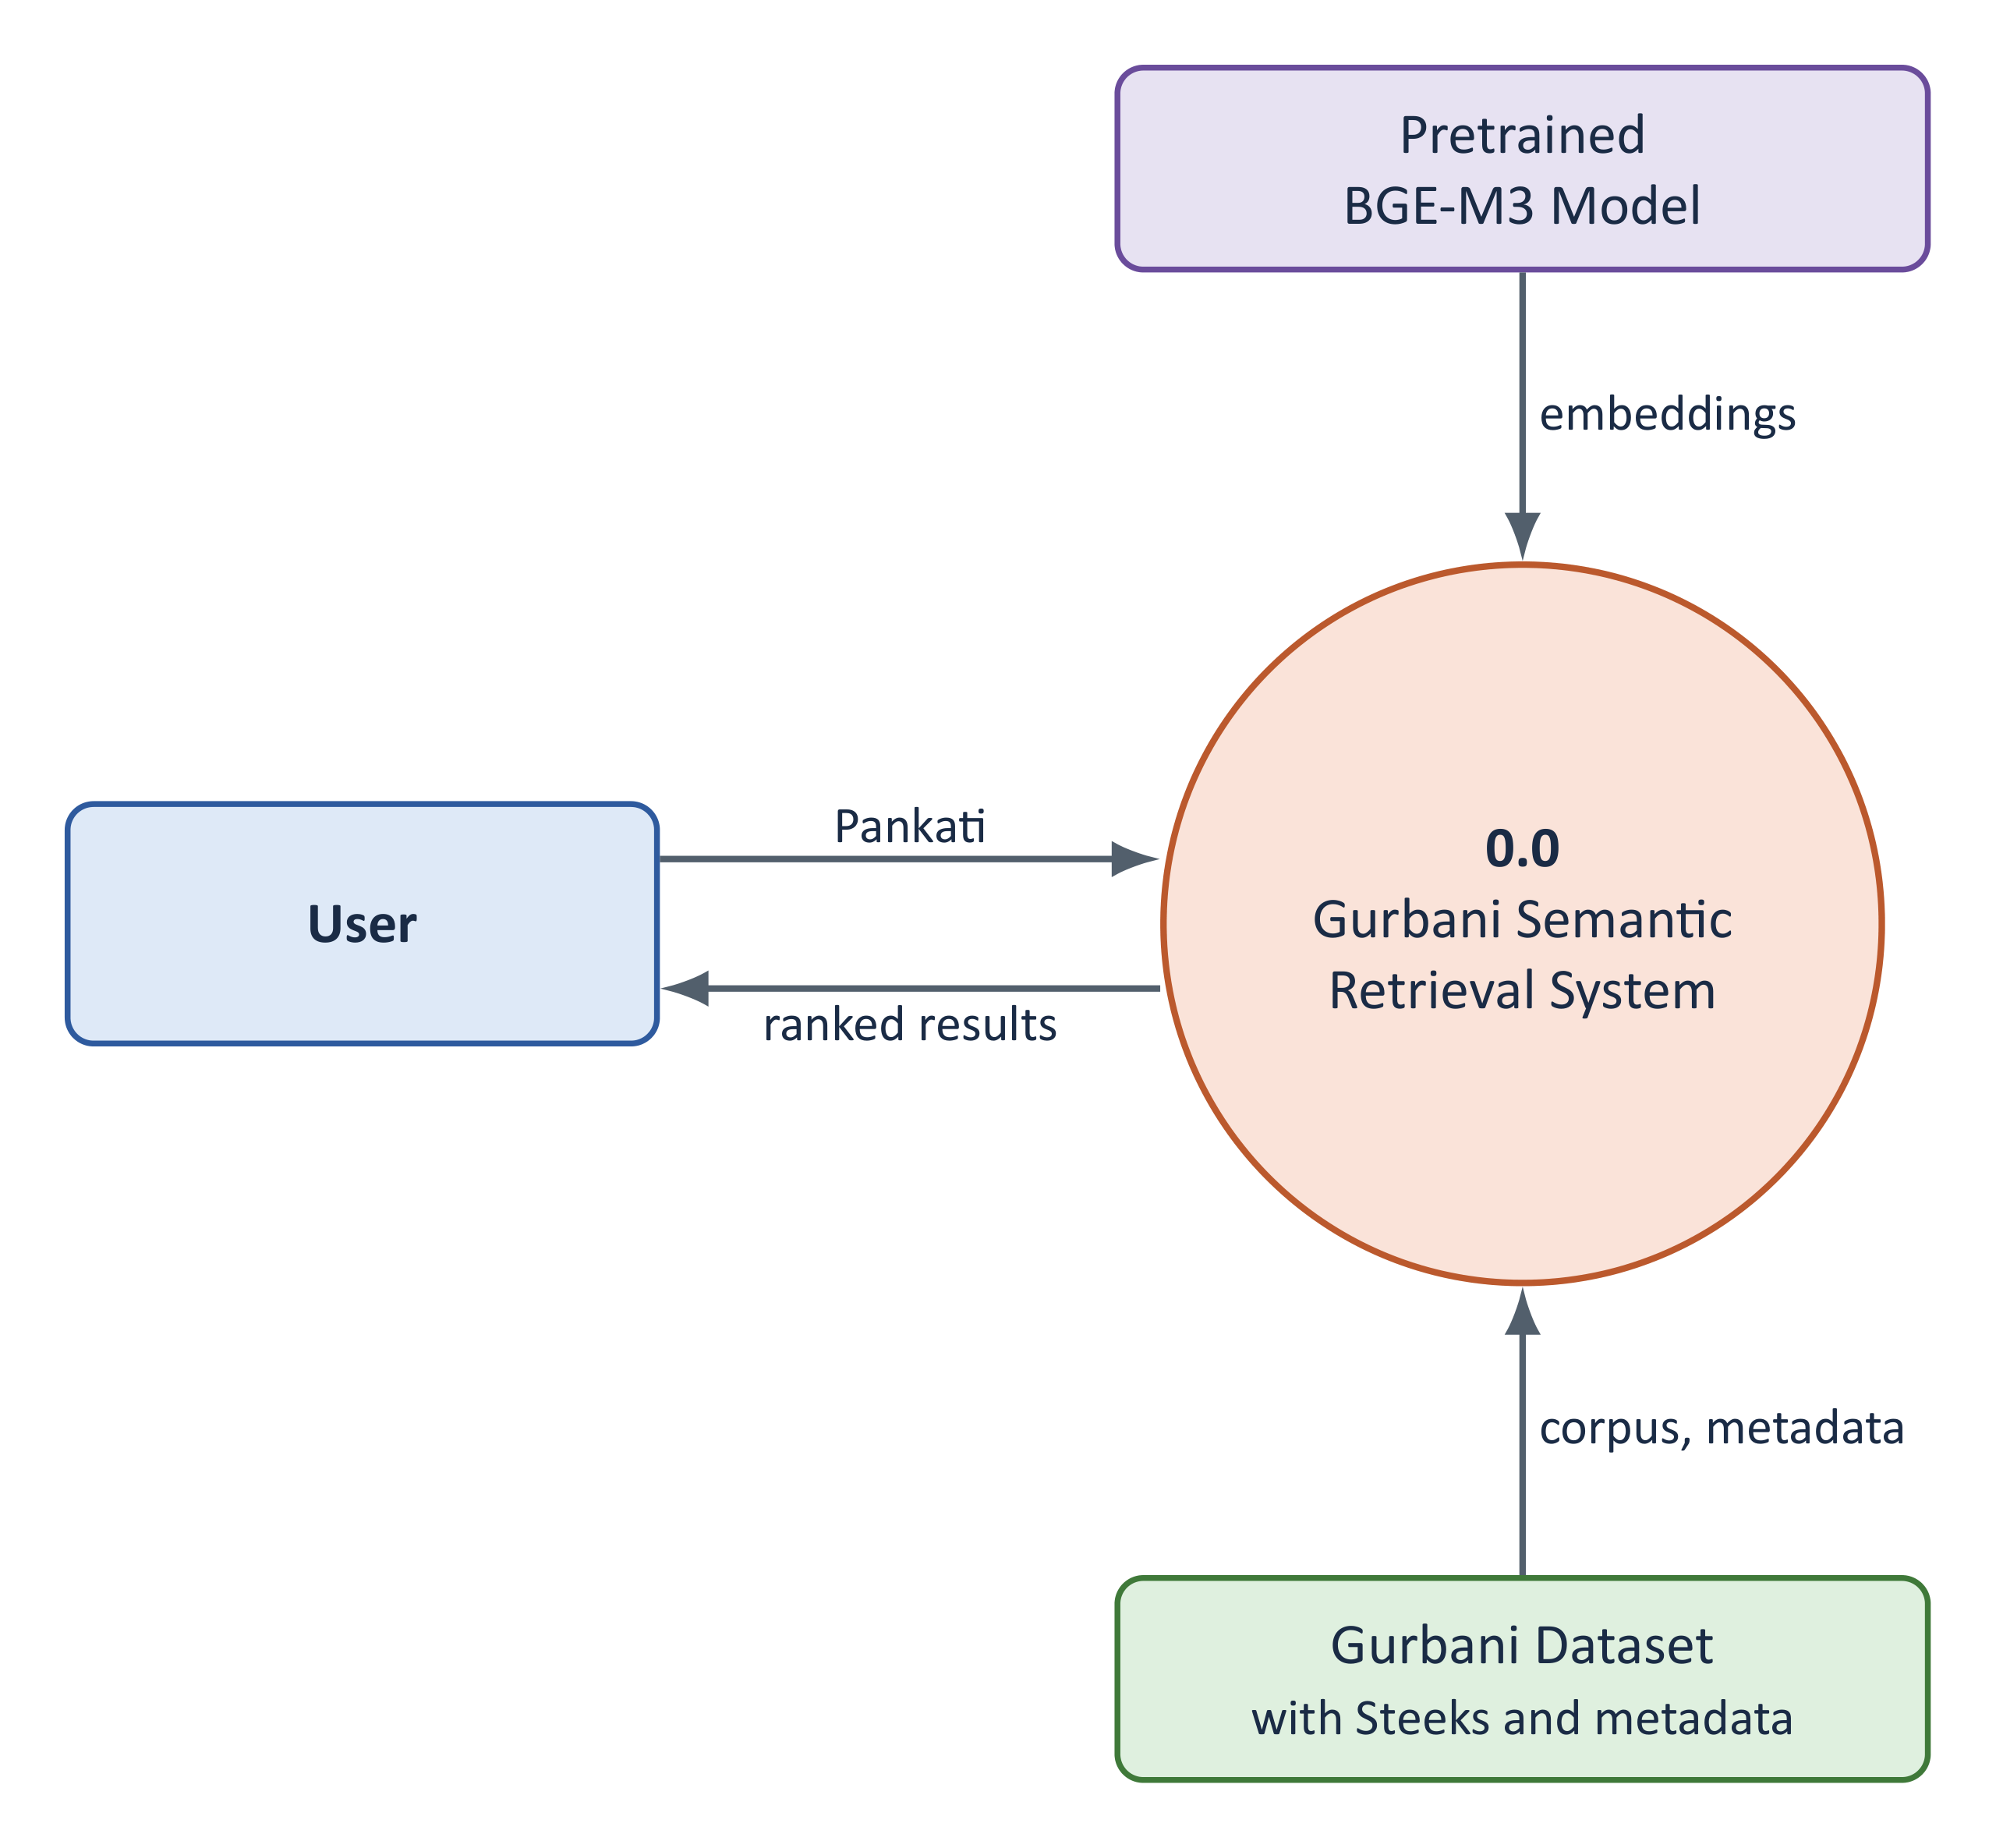
\includegraphics[width=0.90\textwidth]{fig_diag_dfd0.png}
\caption{Data flow diagram, level 0}
\label{fig:dfd0}
\end{figure}

\subsubsection{Level 1}

The level 1 diagram expands the system into its processes and data stores.


\begin{figure}[H]
\centering
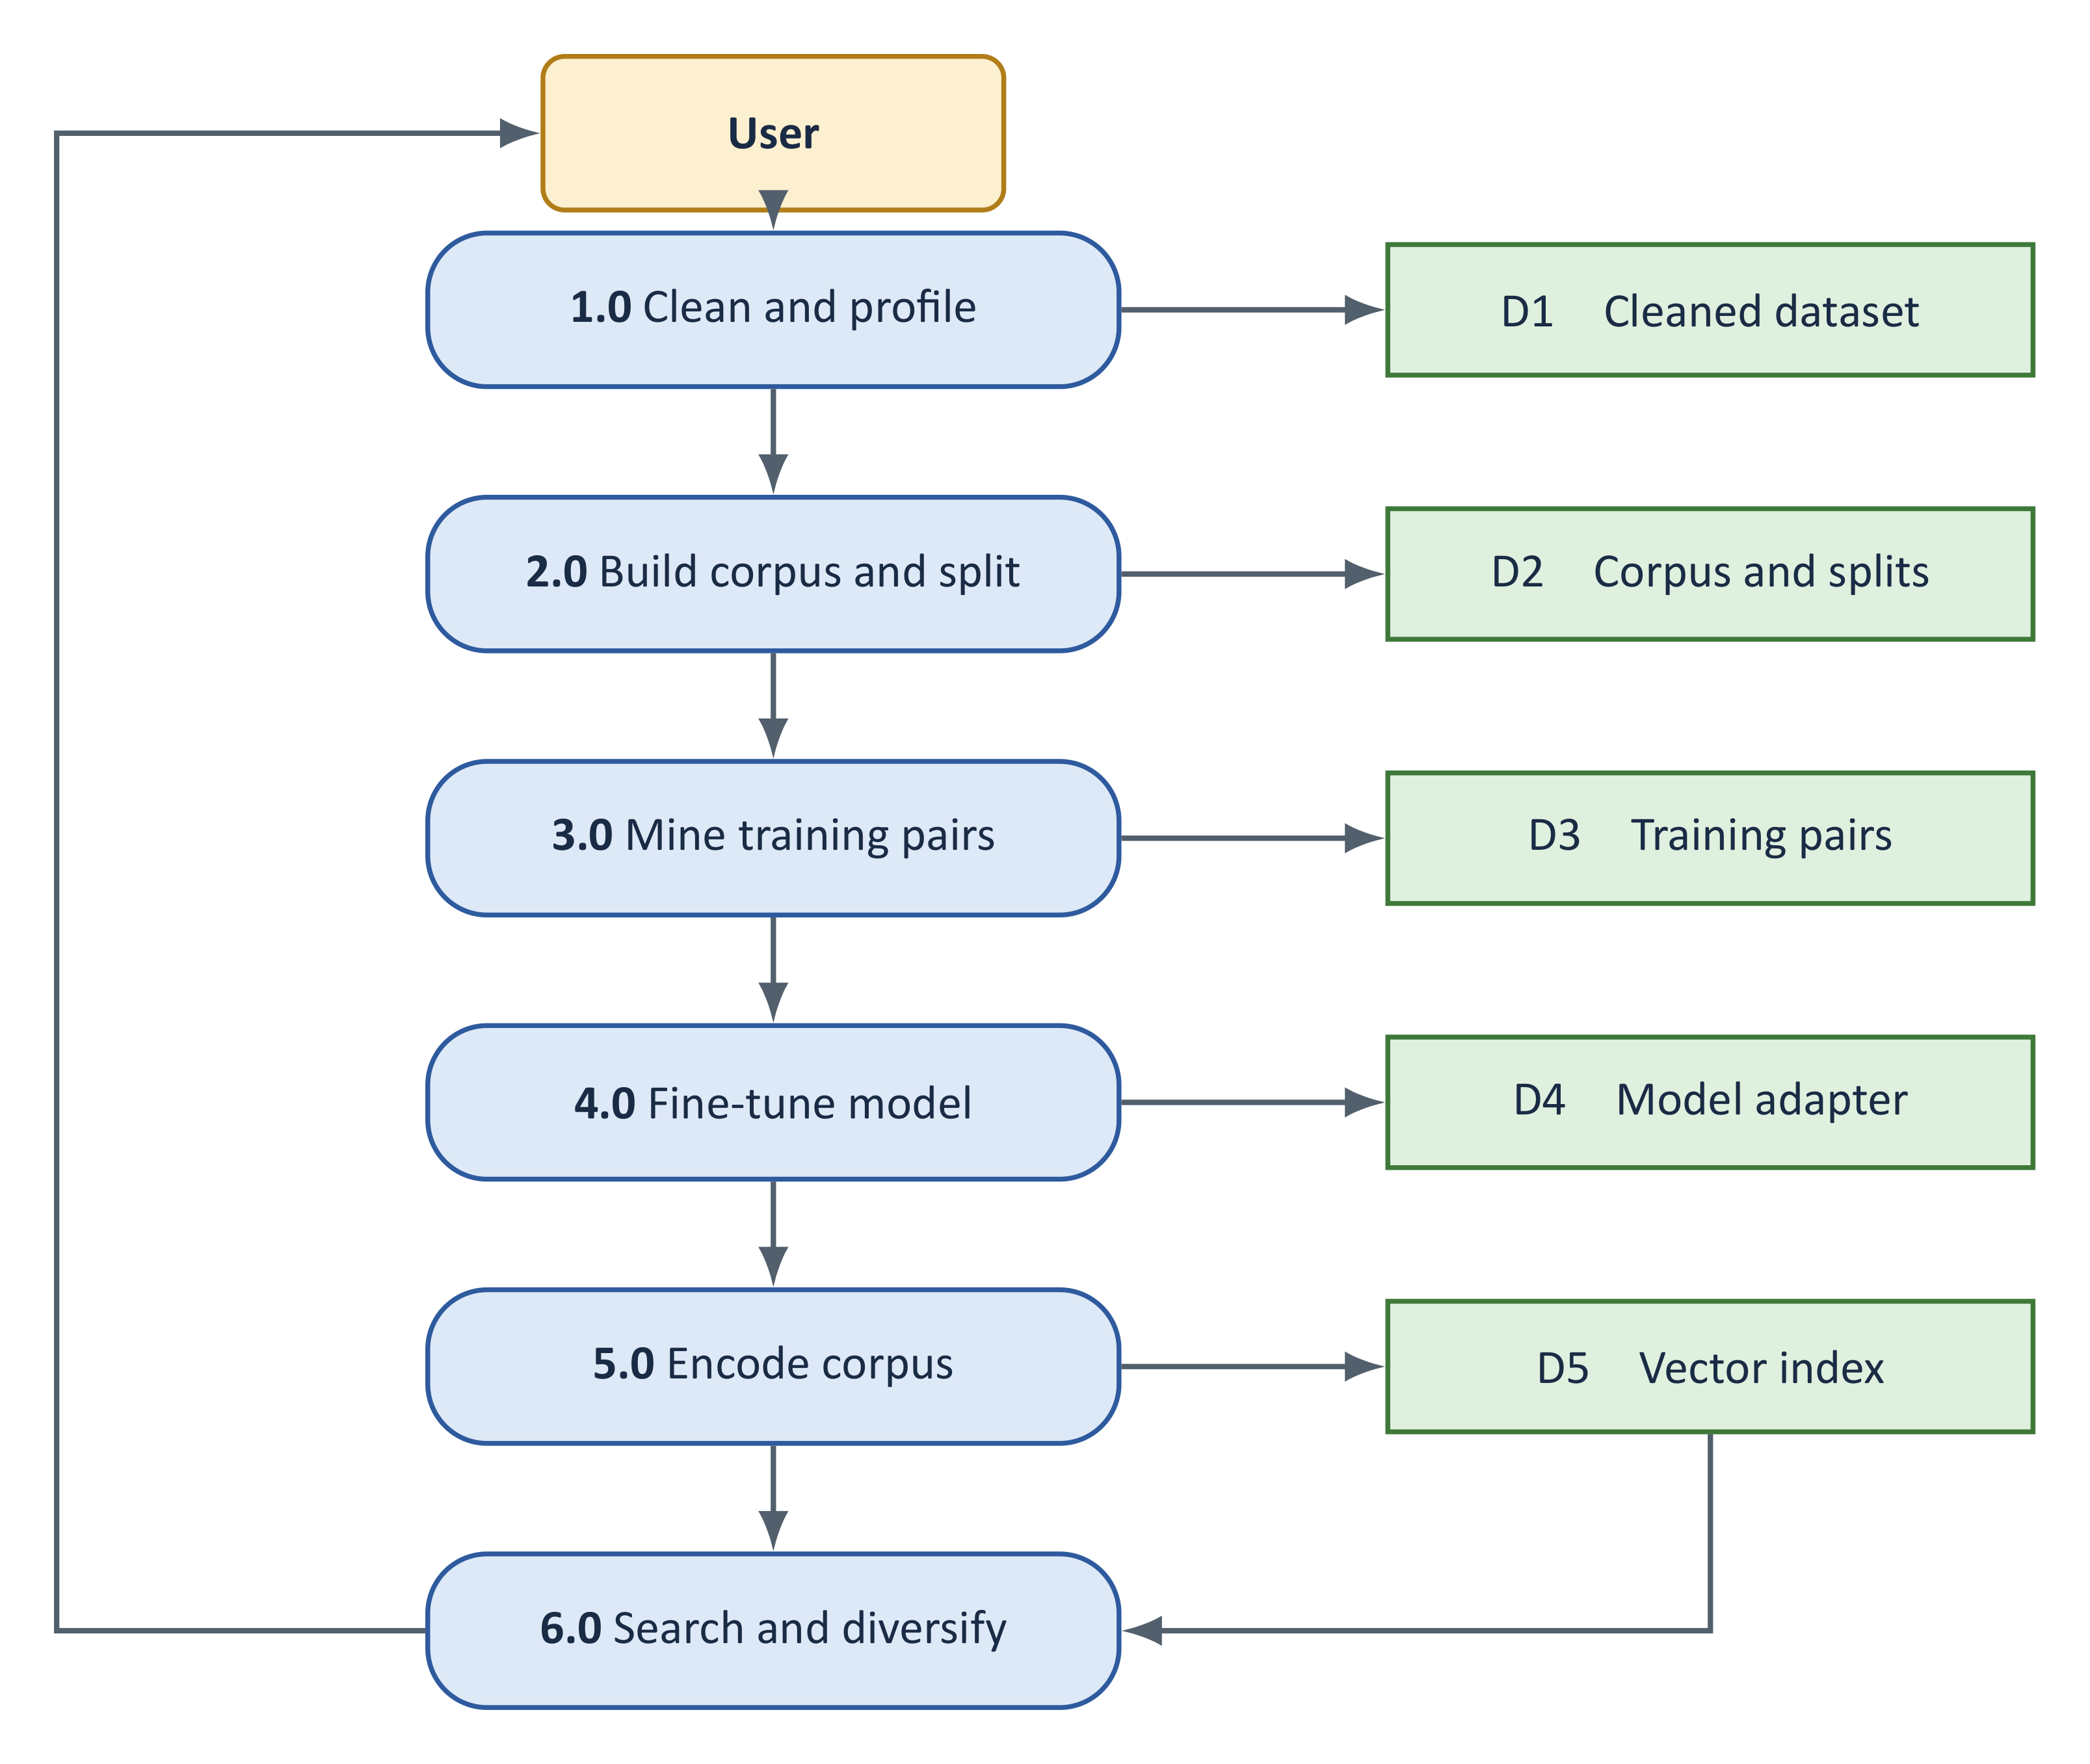
\includegraphics[width=0.95\textwidth]{fig_diag_dfd1.png}
\caption{Data flow diagram, level 1}
\label{fig:dfd1}
\end{figure}

\subsection{Use Case Diagram}


\begin{figure}[H]
\centering
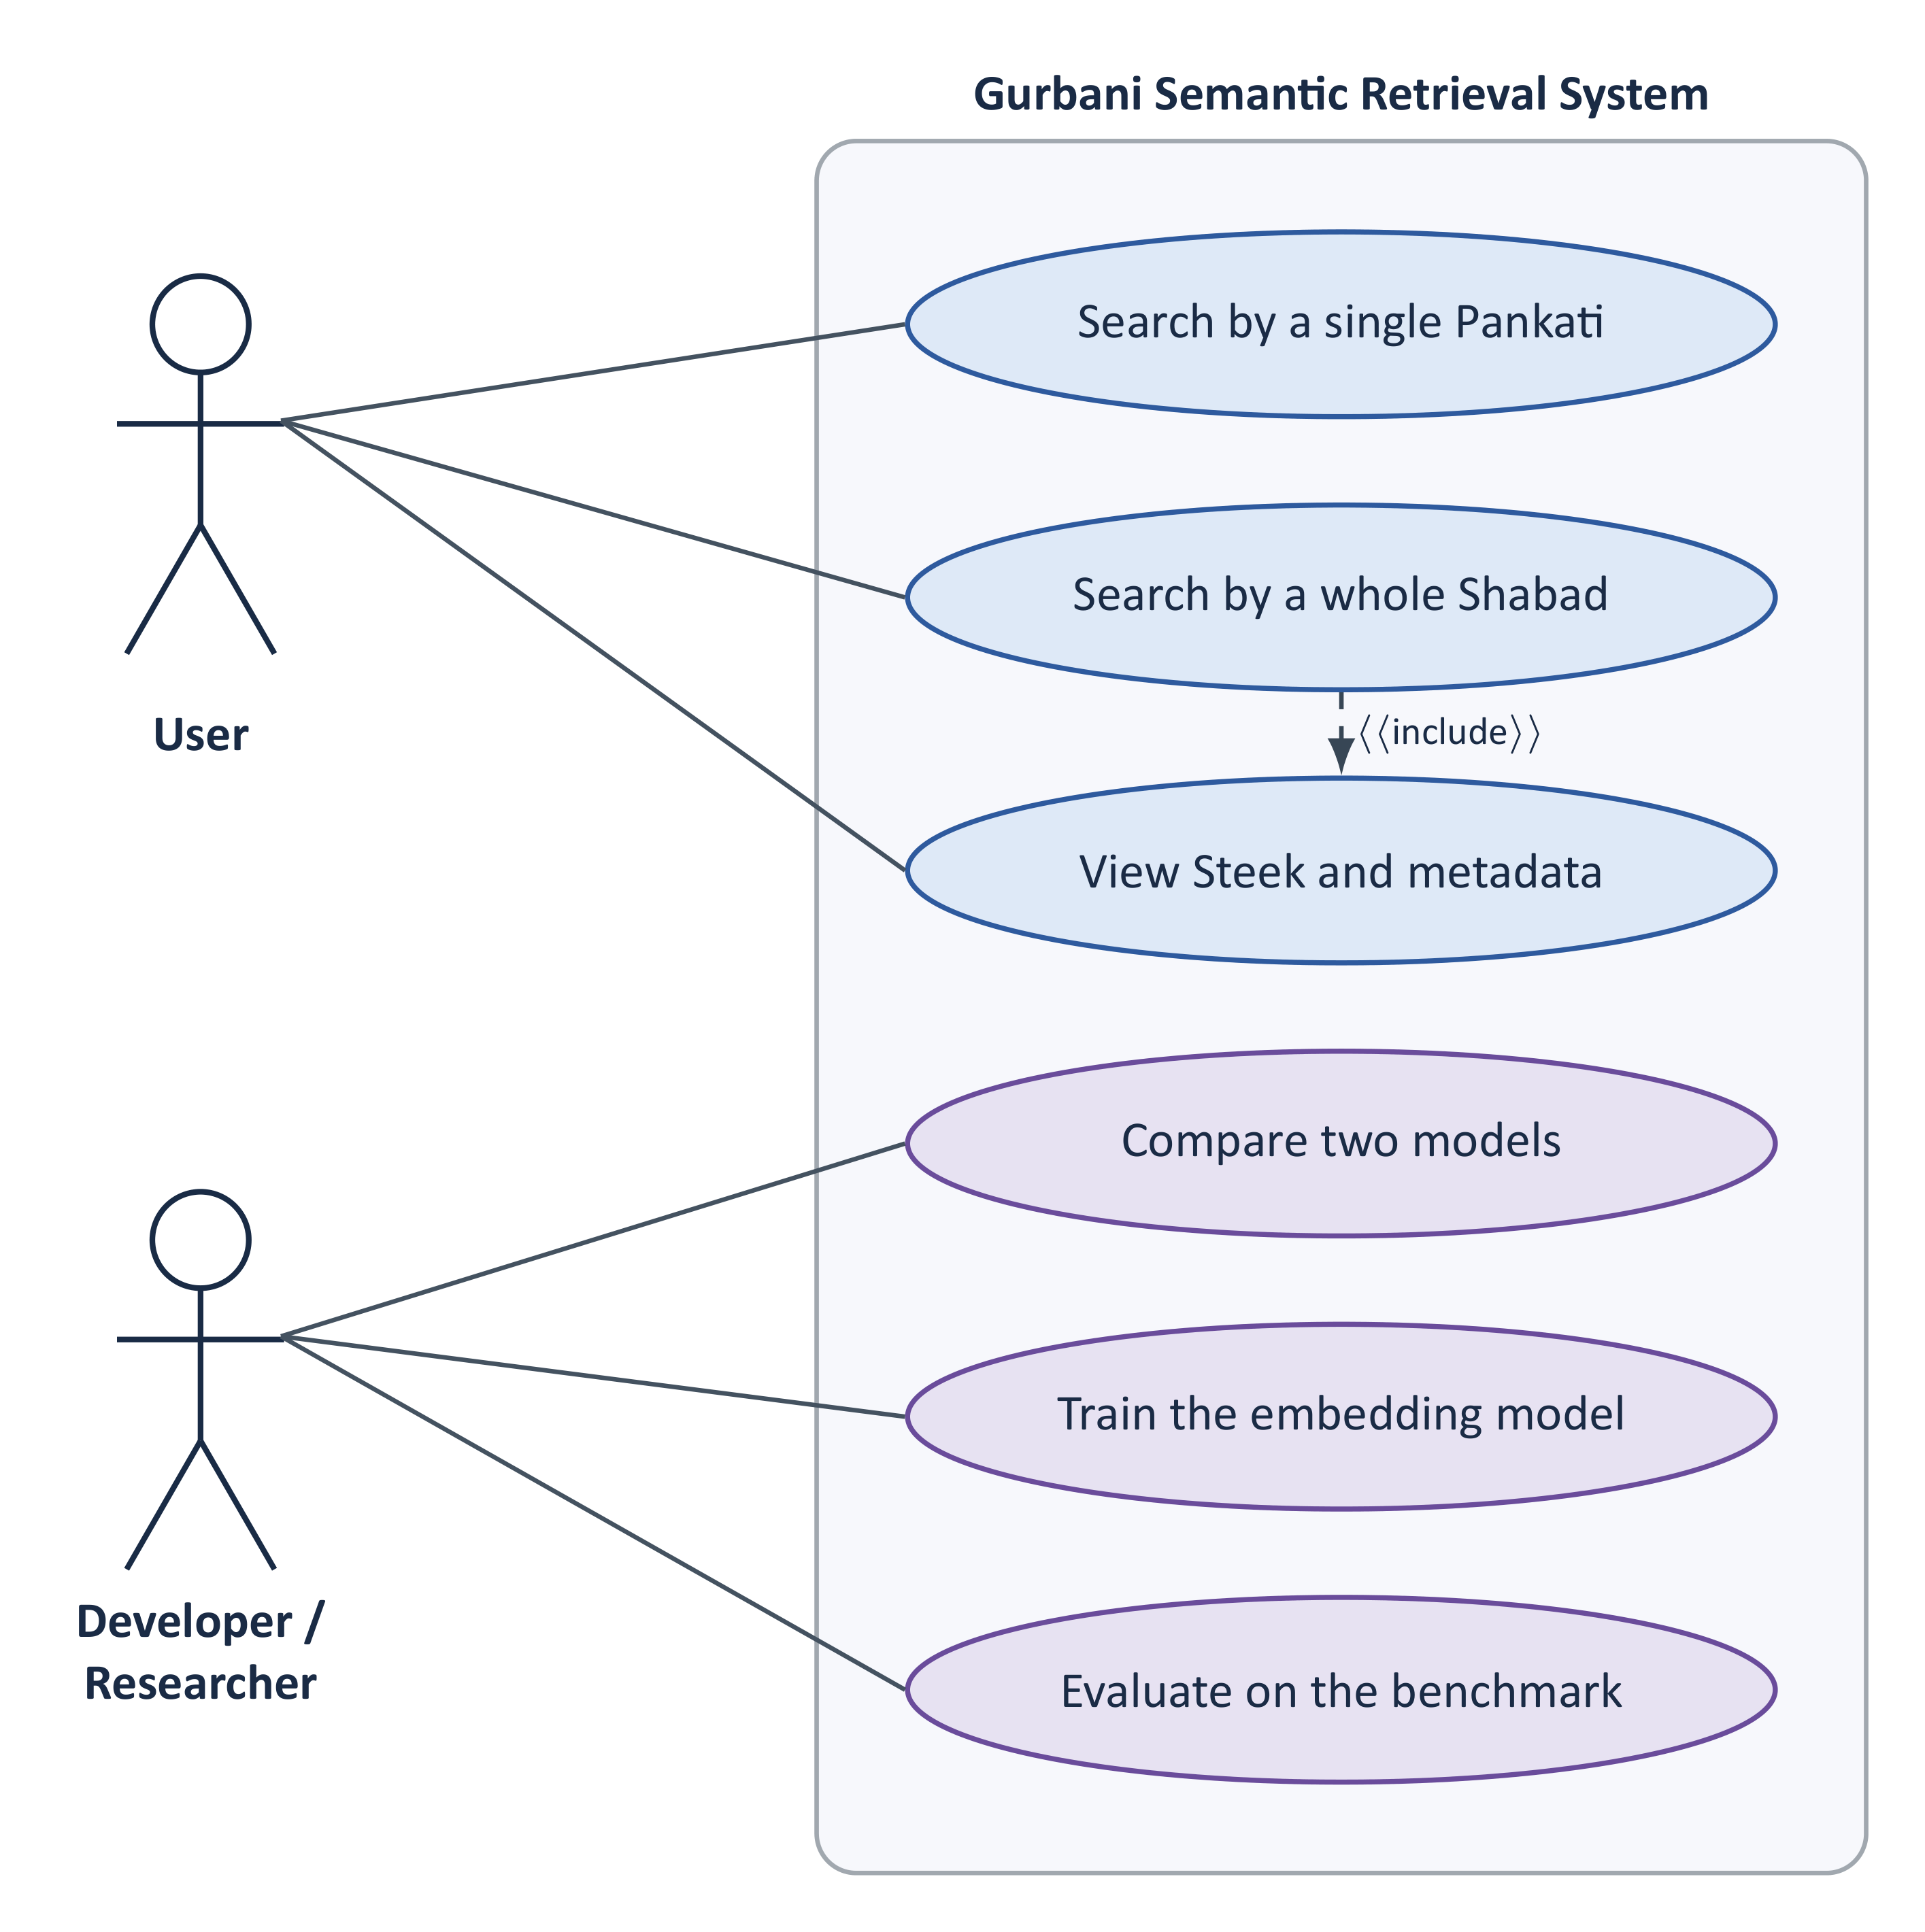
\includegraphics[width=0.85\textwidth]{fig_diag_usecase.png}
\caption{Use case diagram}
\label{fig:usecase}
\end{figure}

\subsection{Sequence Diagram}

The sequence diagram in Figure~\ref{fig:sequence} shows the interaction for a retrieval request. An important design decision is visible here: when the query is a Pankati that already exists in the corpus, its vector is read from the cached index rather than computed, so that the 2.3 GB model need not be loaded at all.


\begin{figure}[H]
\centering
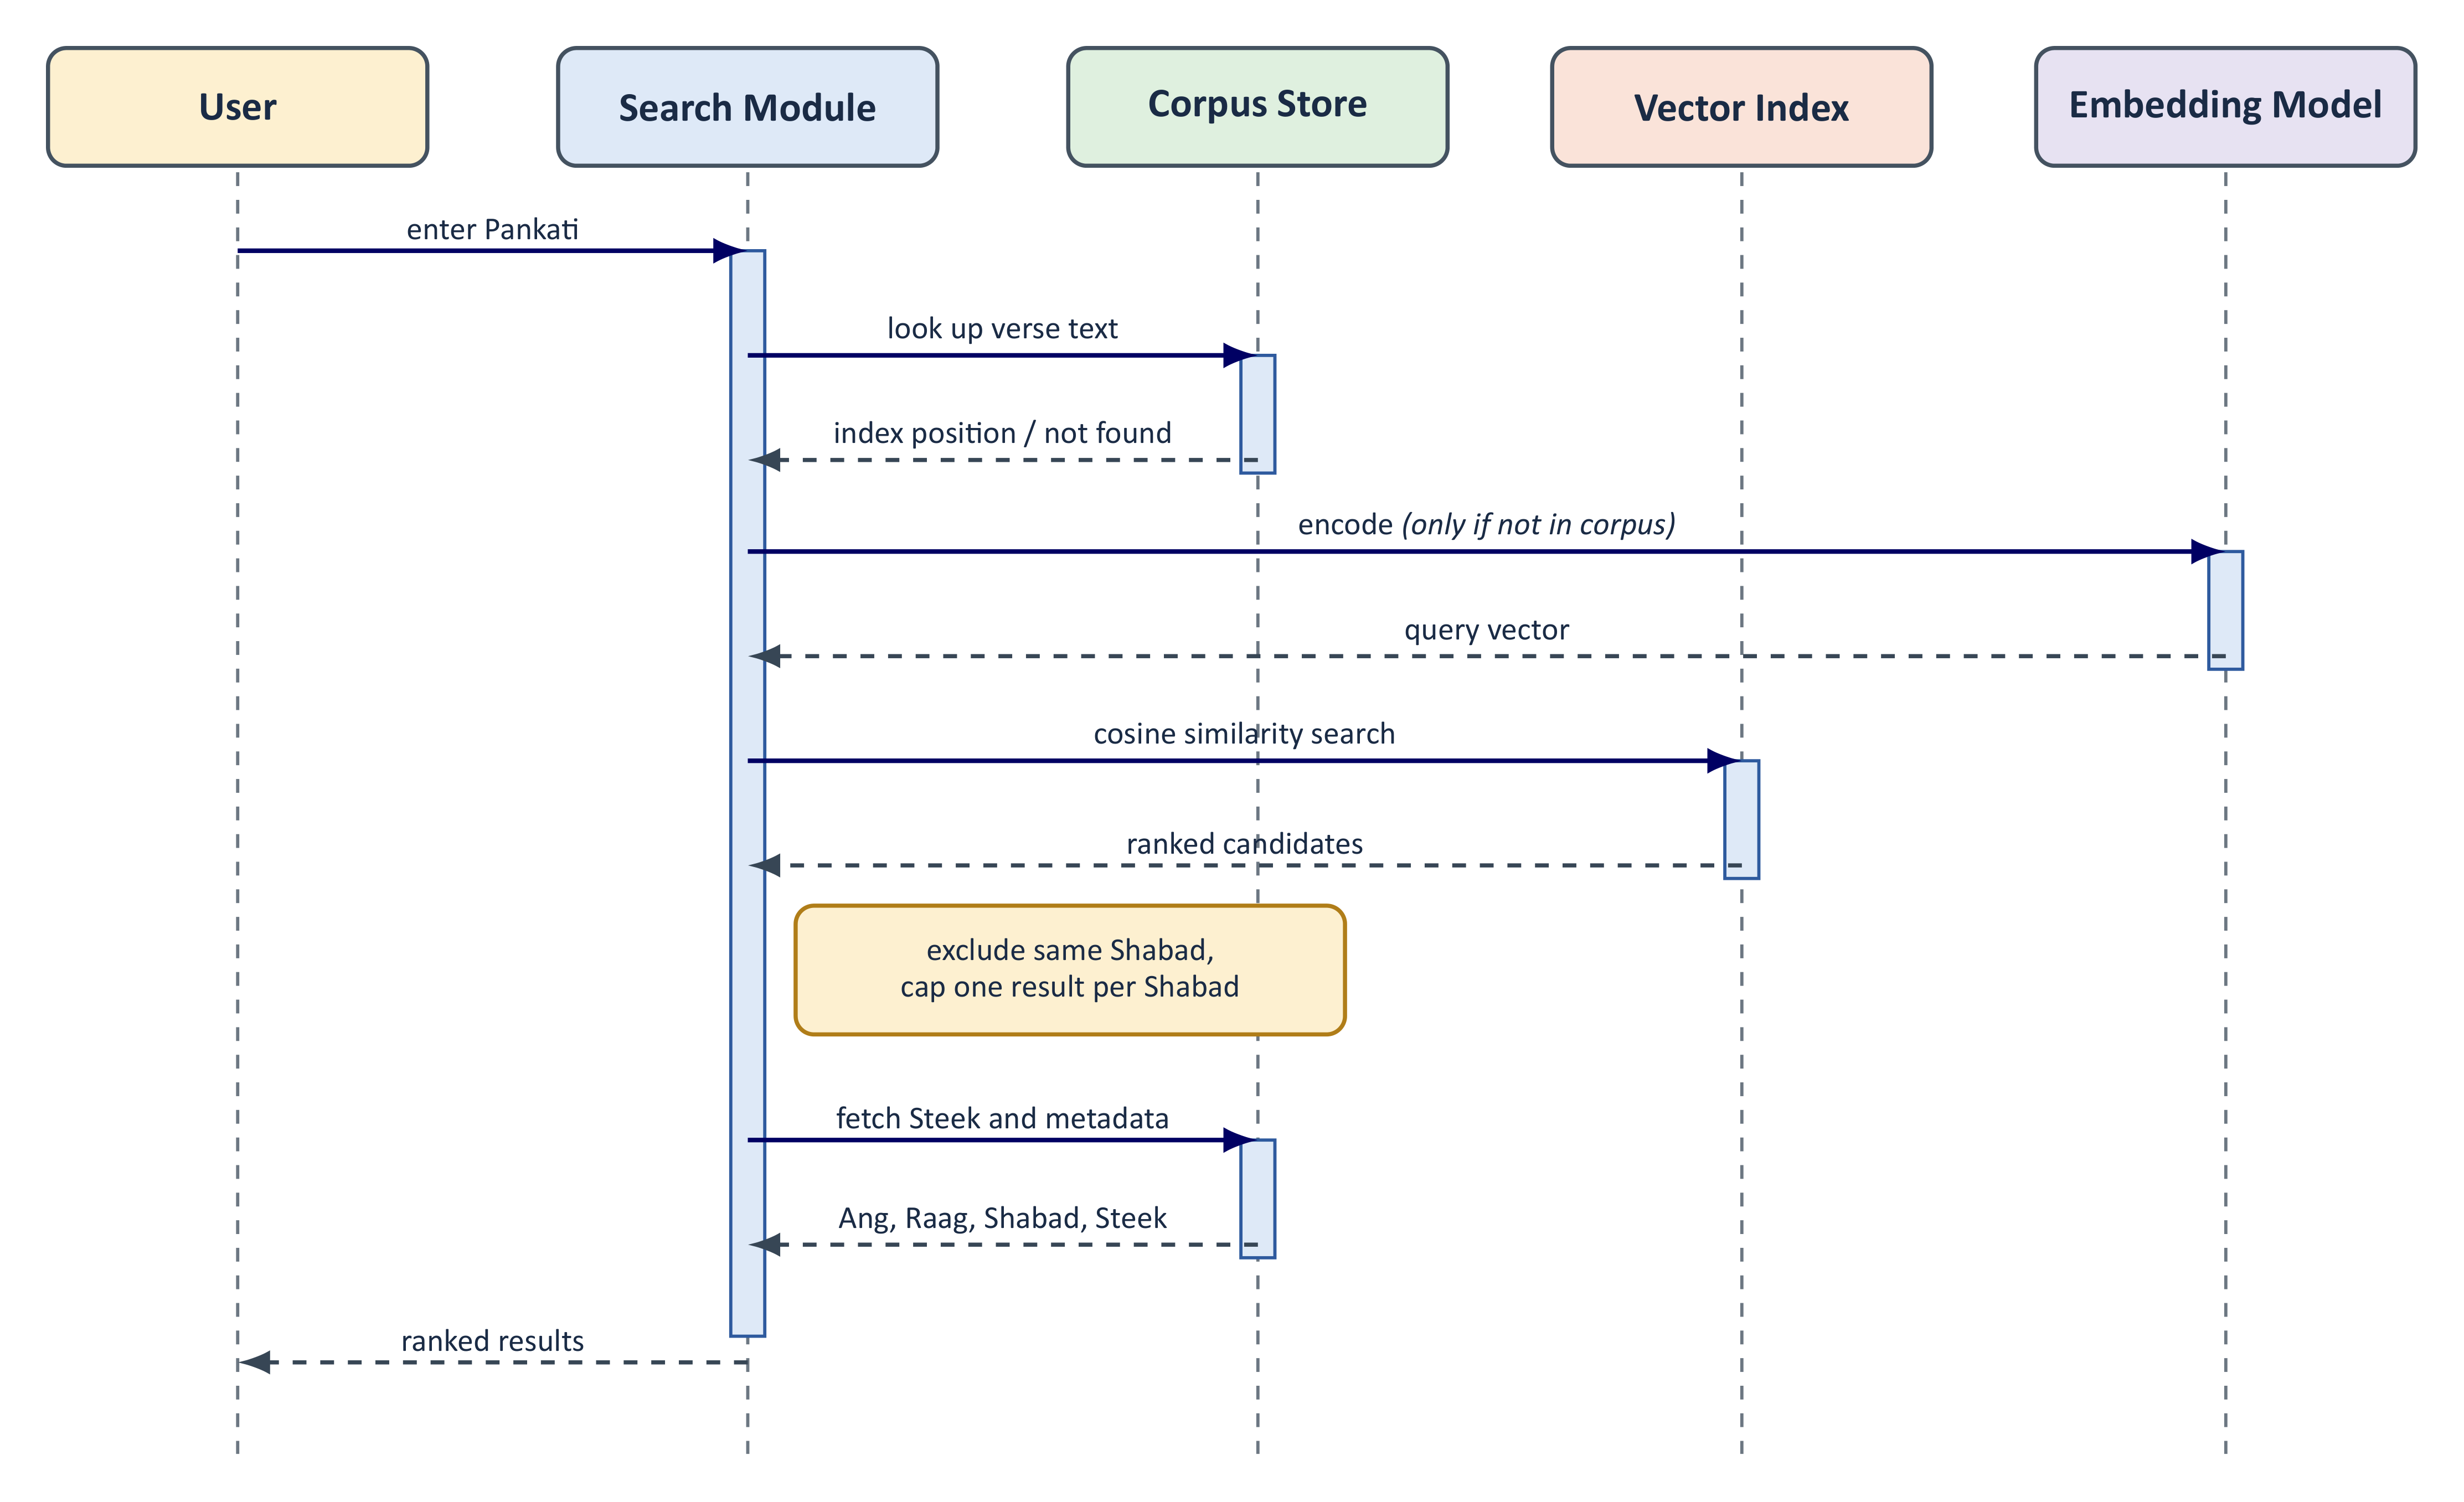
\includegraphics[width=\textwidth]{fig_diag_sequence.png}
\caption{Sequence diagram for a semantic retrieval request}
\label{fig:sequence}
\end{figure}

\subsection{Activity Diagram for Model Training}


\begin{figure}[H]
\centering
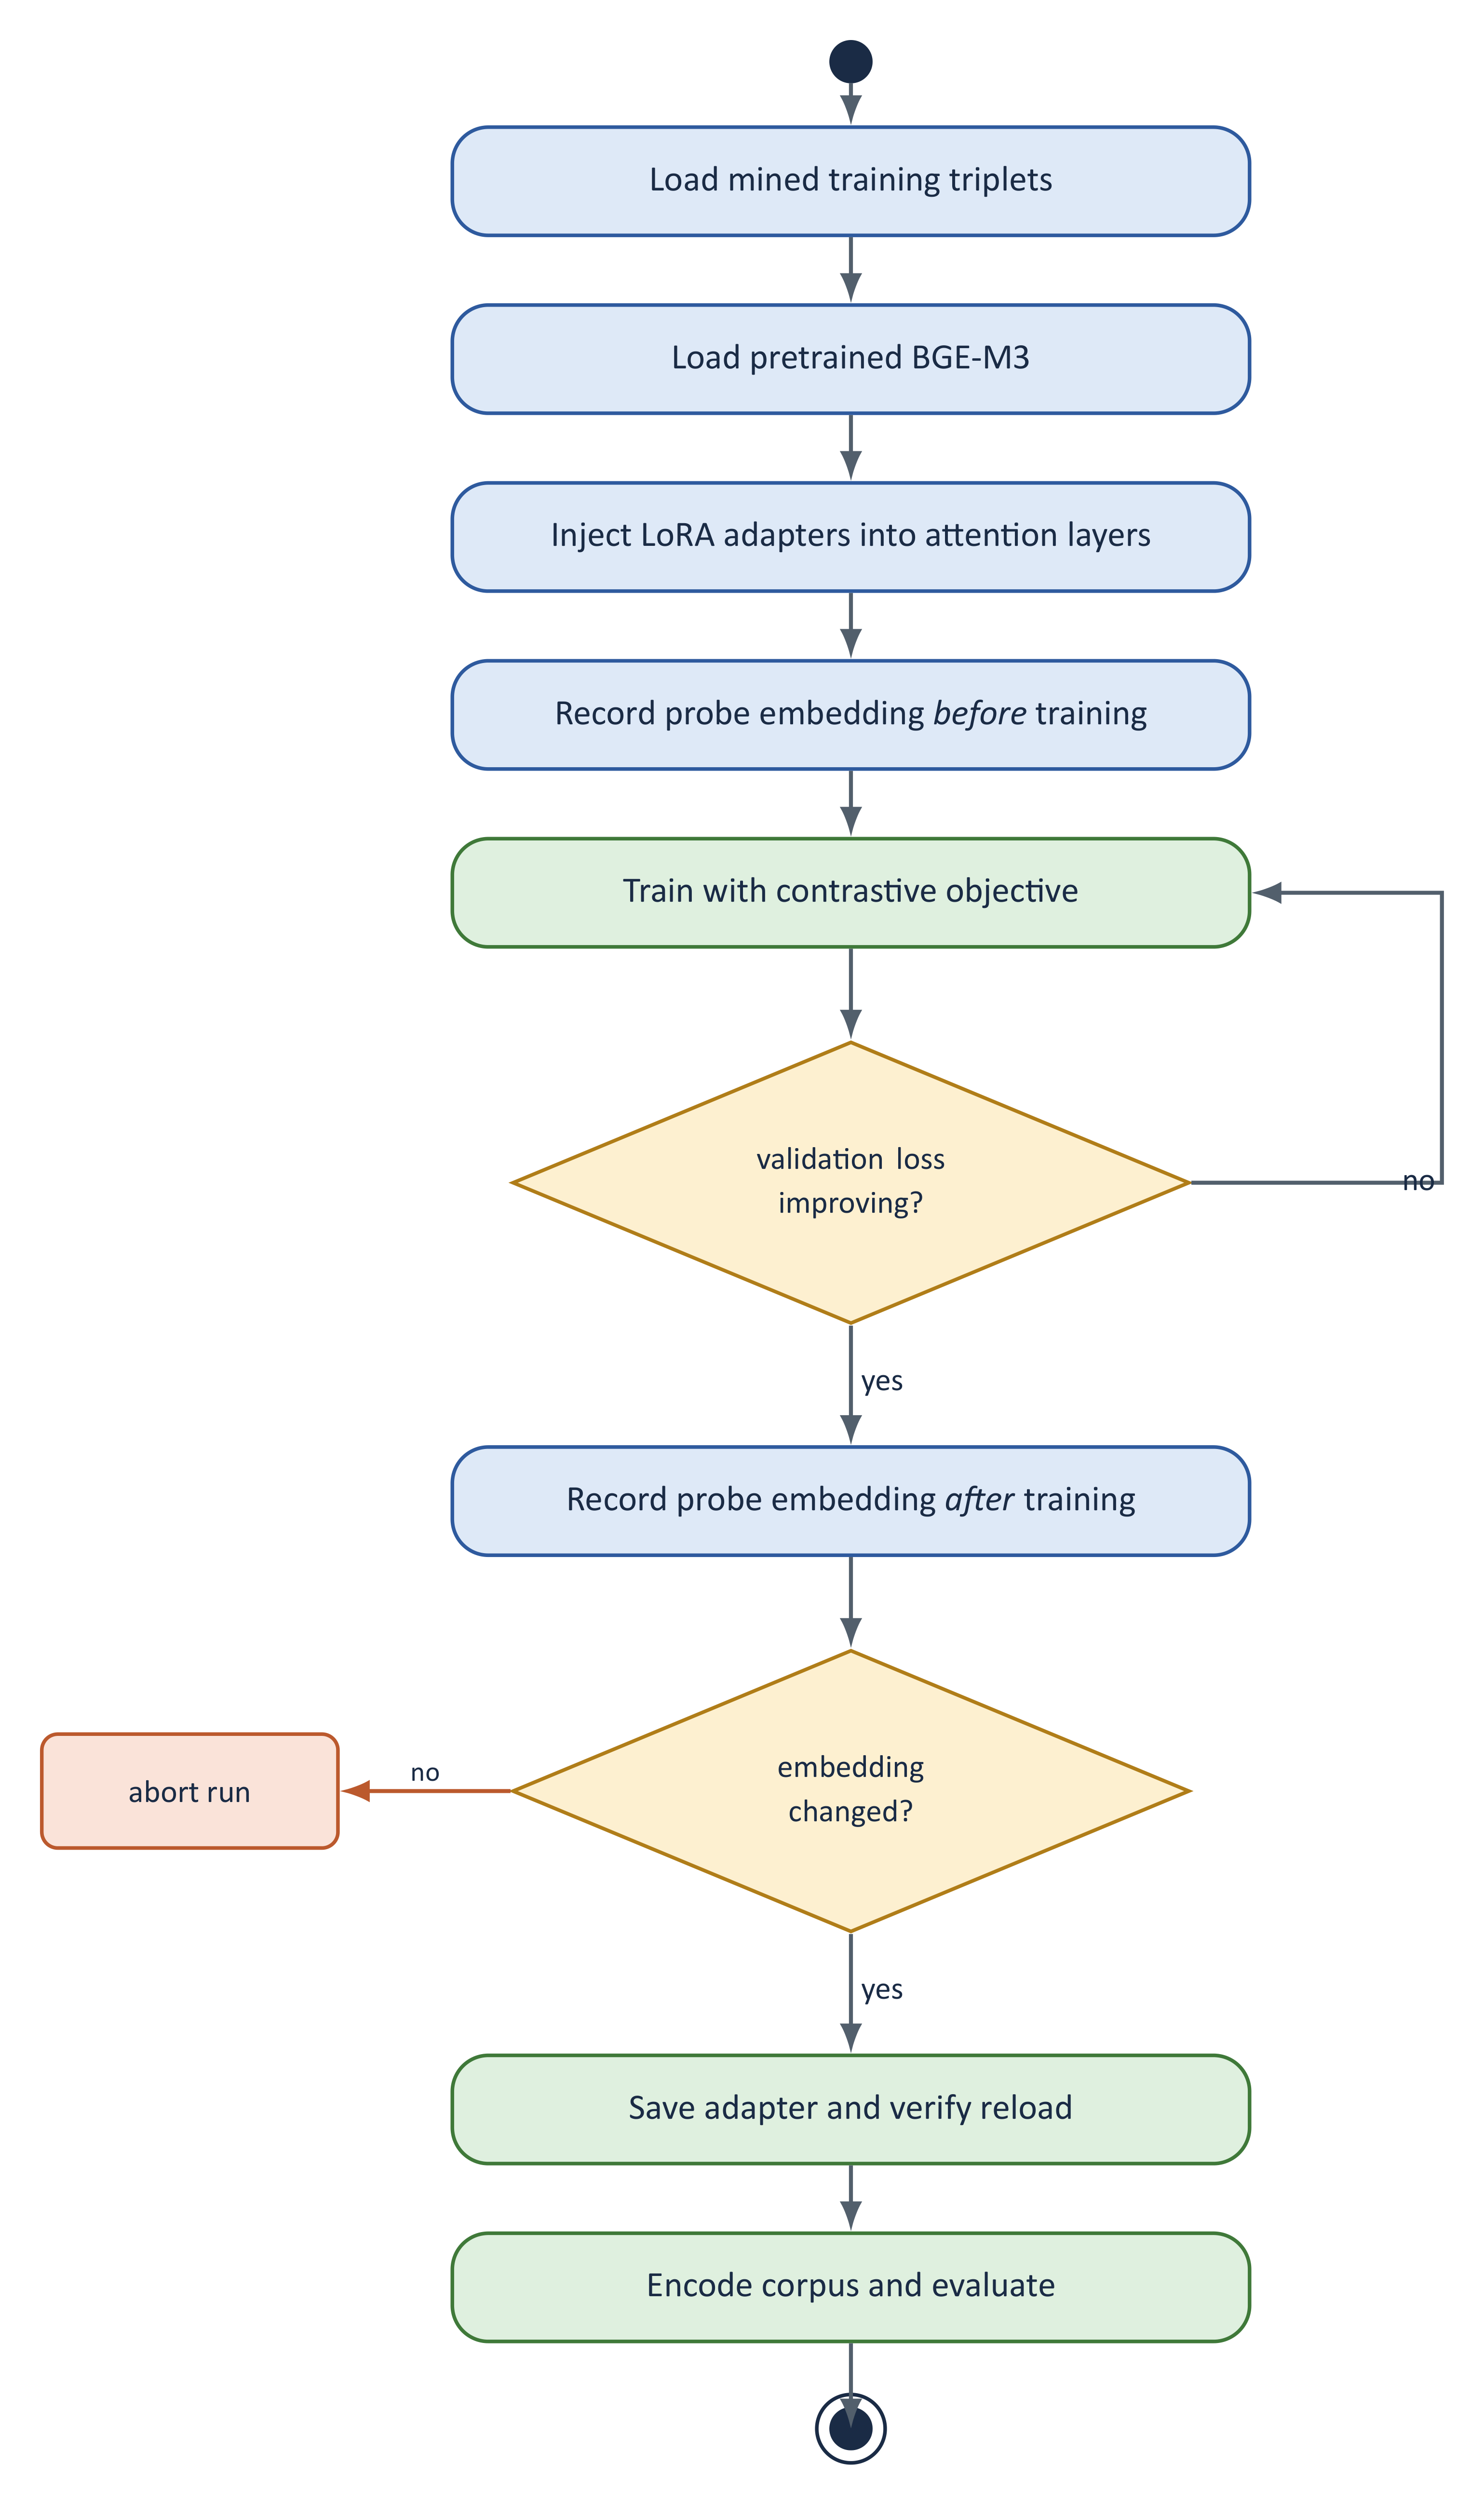
\includegraphics[width=0.69\textwidth]{fig_diag_activity.png}
\caption{Activity diagram for the model training process}
\label{fig:activity}
\end{figure}

\subsection{Module and Component Diagram}


\begin{figure}[H]
\centering
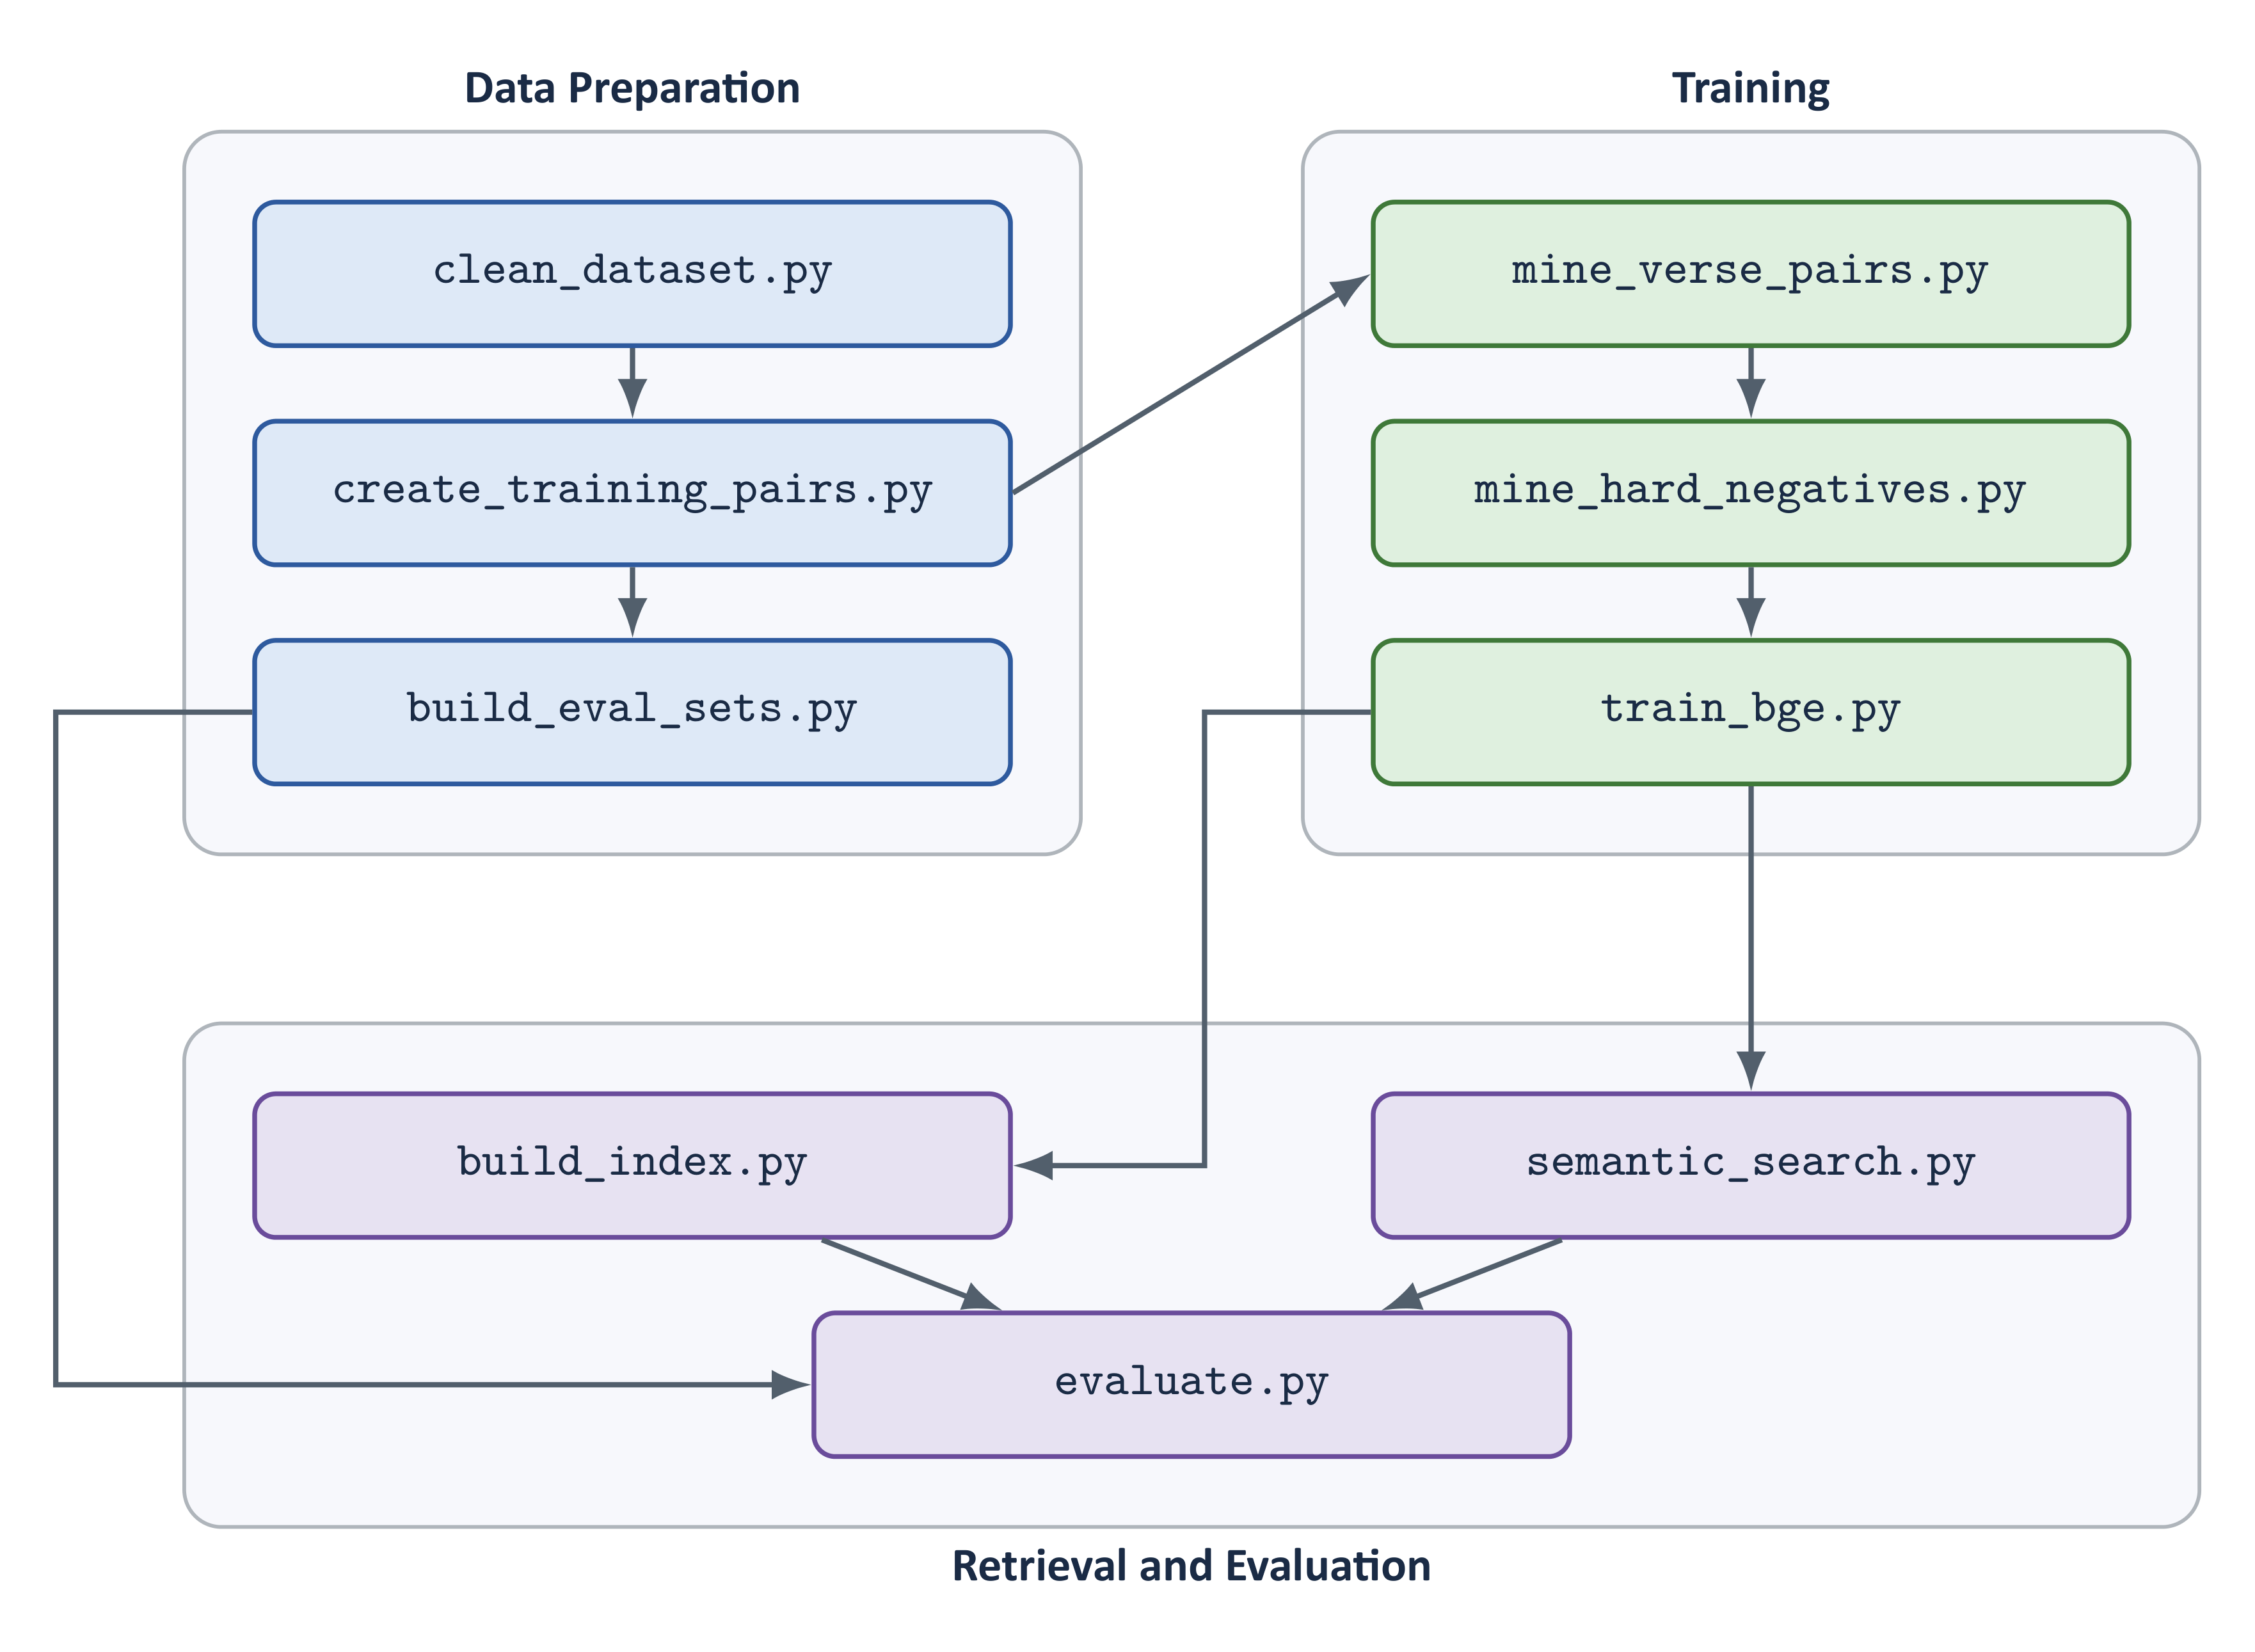
\includegraphics[width=\textwidth]{fig_diag_components.png}
\caption{Module and component diagram}
\label{fig:components}
\end{figure}

\subsection{Deployment Diagram}


\begin{figure}[H]
\centering
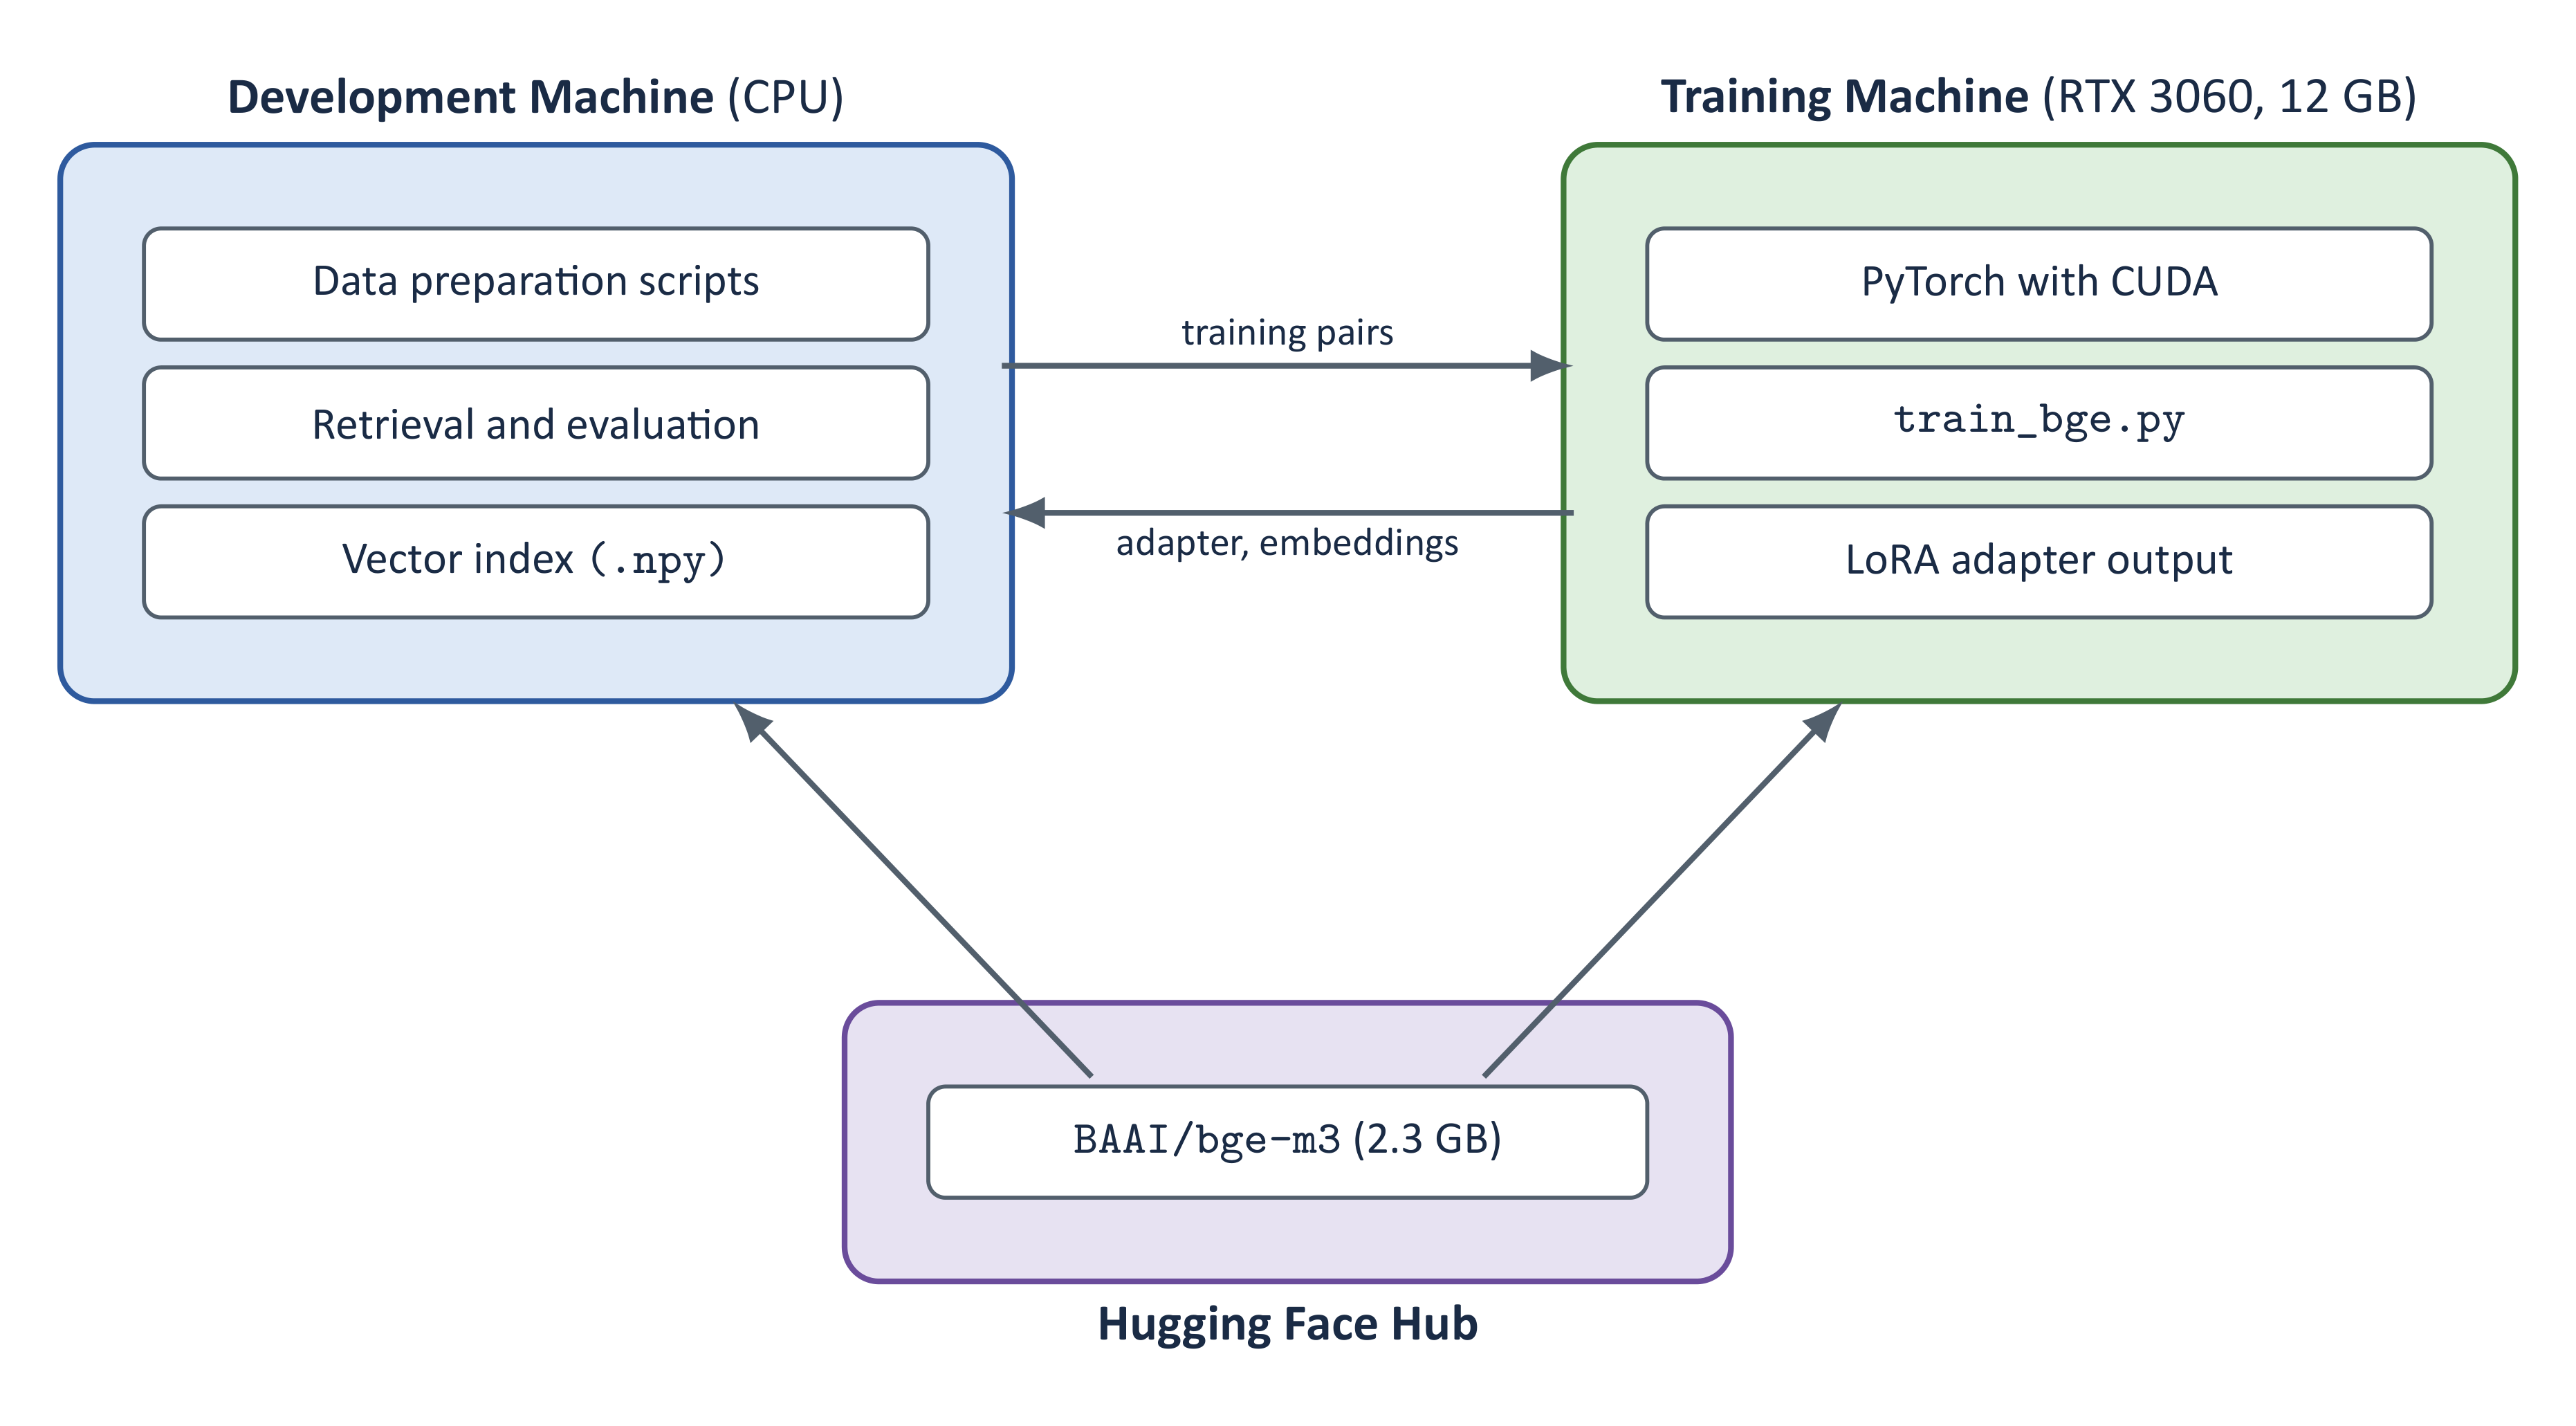
\includegraphics[width=\textwidth]{fig_diag_deployment.png}
\caption{Deployment diagram}
\label{fig:deployment}
\end{figure}

\subsection{Data Design}

The processed data is stored as files rather than in a relational database, because every stage is a batch transformation and no concurrent writes occur. The logical relationships between the entities are nevertheless those of a relational schema, and are shown in Figure~\ref{fig:er}.


\begin{figure}[H]
\centering
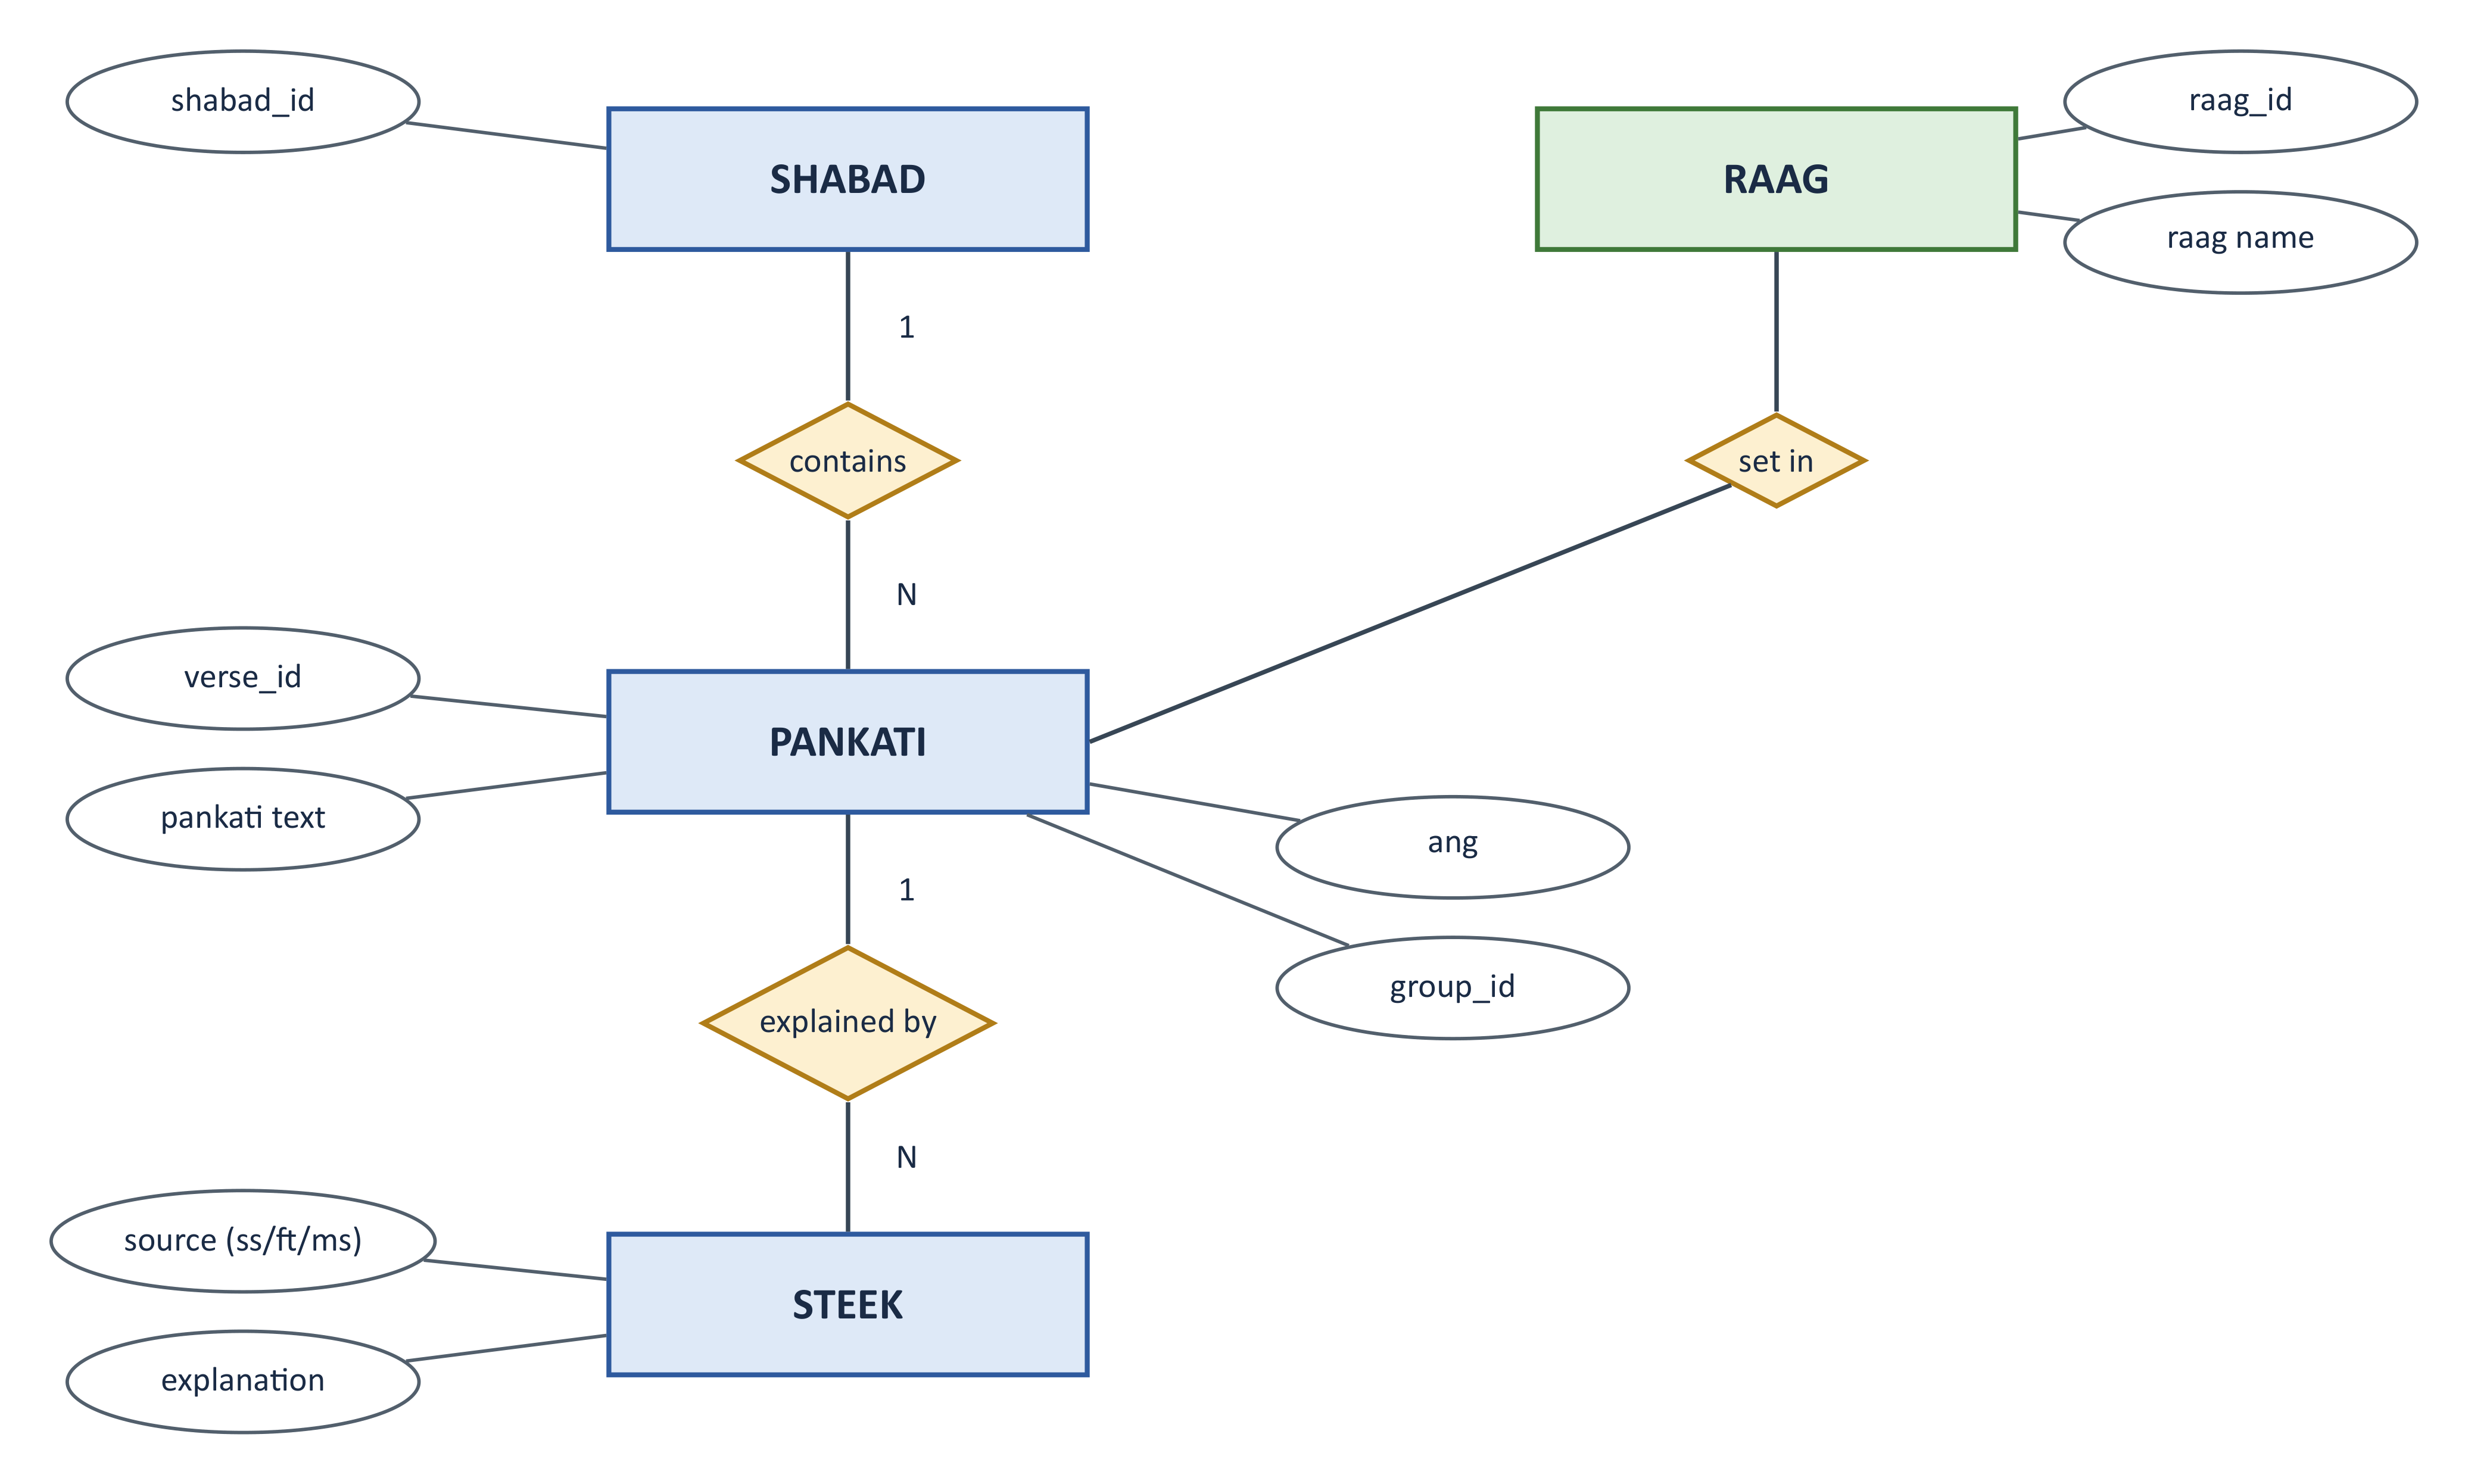
\includegraphics[width=\textwidth]{fig_diag_er.png}
\caption{Data model of the processed corpus}
\label{fig:er}
\end{figure}

\vspace{0.3cm}

\begin{table}[H]
\centering
\renewcommand{\arraystretch}{1.3}
\caption{Principal data files produced by the pipeline}
\begin{tabular}{|p{4.8cm}|p{3.0cm}|p{5.0cm}|}
\hline
\textbf{File} & \textbf{Format} & \textbf{Contents} \\
\hline
cleaned\_gurbani.csv & CSV & All rows with derived flag columns \\
\hline
corpus\_pankatis.jsonl & JSON Lines & 54,844 unique Pankatis with Steeks and metadata \\
\hline
training\_pairs.jsonl & JSON Lines & Pankati--Steek training pairs \\
\hline
verse\_pairs\_hn.jsonl & JSON Lines & Pankati--Pankati triplets with hard negatives \\
\hline
eval\_semantic\_pairs.jsonl & JSON Lines & Evaluation benchmark \\
\hline
embeddings.npy & NumPy array & $54{,}844 \times 1024$ float32 vectors \\
\hline
\end{tabular}
\end{table}

\subsection{Design of the Learning Objective}

The model is trained with a contrastive objective \cite{reimers2019sbert}. For each training example the model is presented with an anchor Pankati, the Pankati that carries the same meaning, and a set of negatives. The objective increases the similarity between the anchor and its positive while decreasing the similarity between the anchor and every negative. The negatives are of two kinds. In-batch negatives are the other Pankatis present in the same batch, which are inexpensive but easy to distinguish. Hard negatives are mined deliberately: Pankatis that share a large proportion of their vocabulary with the anchor but are explained differently by the commentators. These prevent the model from succeeding through keyword overlap alone.


\begin{figure}[H]
\centering
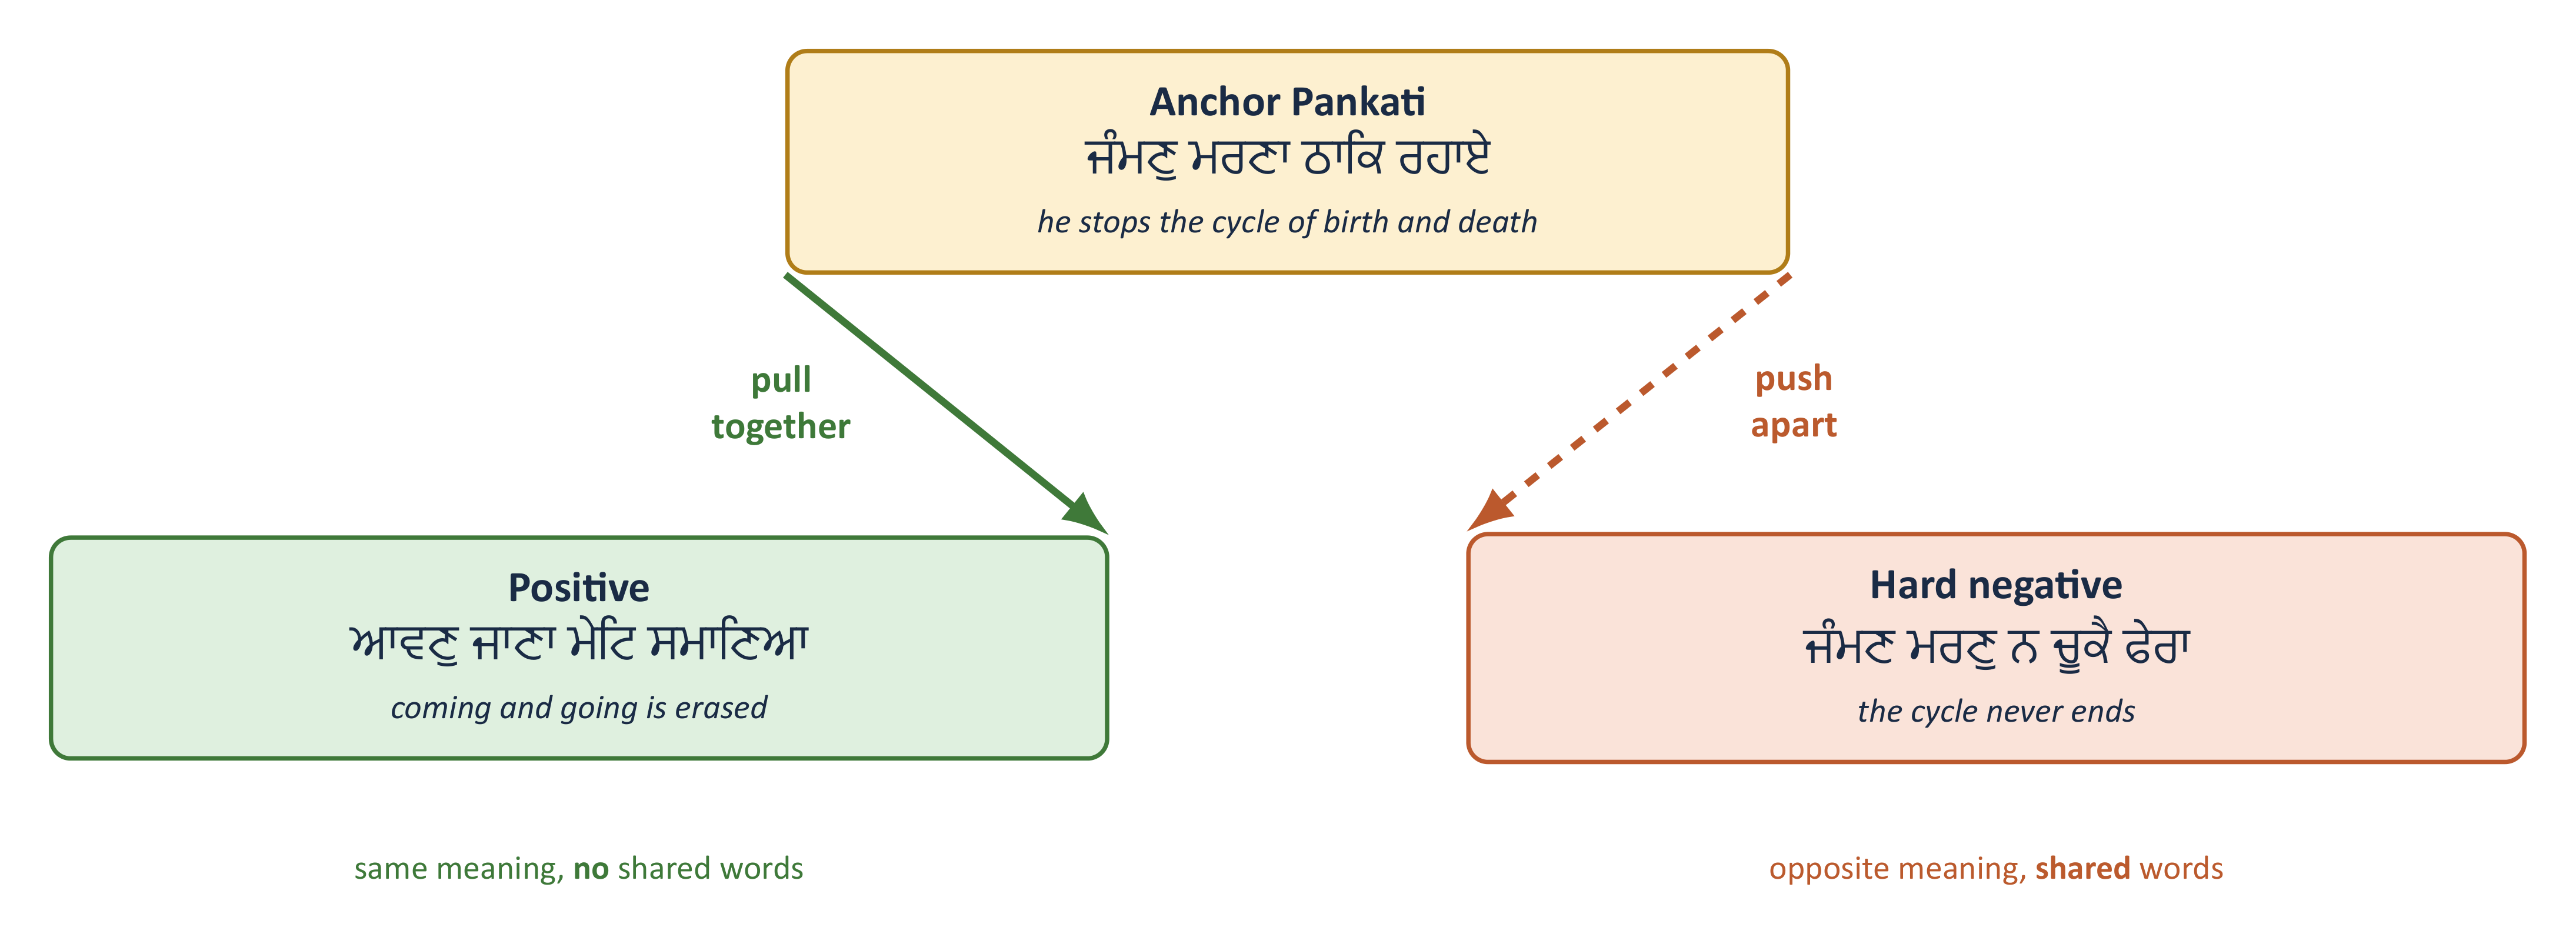
\includegraphics[width=\textwidth]{fig_diag_contrastive.png}
\caption{Contrastive learning objective with a mined hard negative}
\label{fig:contrastive}
\end{figure}

\subsection{Design of the Evaluation Benchmark}

Because no labelled verse-to-verse similarity data exists, the benchmark is mined. A pair of Pankatis is accepted as a gold pair when two independent commentators, Sahib Singh and Manmohan Singh, both explain them in similar terms. Requiring agreement between two authors of different periods and styles removes pairs that match only on formulaic phrasing such as the attribution \textit{``\gur{ਕਬੀਰ ਆਖਦਾ ਹੈ}''}. Gold pairs are restricted to different Shabads, and word overlap between the two verses is recorded but never used as a filter, since the criterion is identity of meaning and not difference of wording.

\subsection{Design Decisions Protecting the Validity of Results}

\noindent\textbf{Grouped partitioning.}
The dataset is not split at random. A union-find structure groups together every pair of rows that share a Shabad, that have identical Pankati text, or that have identical Steek text, and whole groups are assigned to a partition. Without this, consecutive lines of one Shabad would appear on both sides of the split and the measured improvement would reflect leakage rather than learning.

\vspace{0.3cm}

\noindent\textbf{Exclusion of duplicated commentaries.}
Measurement showed that \texttt{steek\_bdb} is byte-identical to \texttt{steek\_ss} in 99.9 per cent of rows, and that \texttt{steek\_pss} is a word-glossary rather than a paraphrase. Both are excluded from training so that no Pankati receives double weight and no glossary structure is learned, while both are retained in the corpus for display.

% ===================== TESTING MODULE =====================
\newpage
\section{Testing Module}
\addcontentsline{toc}{section}{Testing Module}

Testing a semantic retrieval system differs from testing a conventional application, because the correctness of a result is a matter of meaning rather than of a fixed expected value. The testing strategy therefore combines conventional software testing of the pipeline stages with quantitative retrieval evaluation and qualitative inspection.

\subsection{Testing Techniques Proposed}

\noindent\textbf{Unit testing of text-processing rules.}
The heading detector and the tokeniser operate on Gurmukhi text, where incorrect behaviour is not visible by inspection. Each rule is therefore tested against a list of lines whose correct classification is known in advance, containing both headings and genuine verses chosen to be adversarial.

\vspace{0.3cm}

\noindent\textbf{Integrity testing of the data pipeline.}
After each stage, the output is checked for structural correctness: row counts must reconcile, no partition may share a Shabad with another, and the number of embeddings must equal the number of corpus entries.

\vspace{0.3cm}

\noindent\textbf{Leakage testing.}
Every pair of partitions is tested for overlap in Pankati text, Shabad identifier, leakage-group identifier and Steek text. All four counts must be zero.

\vspace{0.3cm}

\noindent\textbf{Retrieval evaluation.}
The system is scored on the mined benchmark using standard information-retrieval measures: Hit@$k$, Mean Reciprocal Rank and normalised Discounted Cumulative Gain. Keyword baselines \cite{robertson2009bm25} are scored on identical queries so that differences are attributable to the retrieval method alone.

\vspace{0.3cm}

\noindent\textbf{Ablation testing.}
Each design change is evaluated as a separate model and scored on the same benchmark, so that its contribution can be isolated.

\vspace{0.3cm}

\noindent\textbf{Qualitative testing.}
A fixed list of query Pankatis with known correct answers is used for manual inspection of the ranked output.

\subsection{Test Cases}

\begin{table}[H]
\centering
\renewcommand{\arraystretch}{1.25}
\caption{Test cases executed}
\begin{tabular}{|c|p{5.1cm}|p{5.3cm}|c|}
\hline
\textbf{ID} & \textbf{Test case} & \textbf{Expected result} & \textbf{Status} \\
\hline
T-01 & Classify \textit{\gur{ਪਉੜੀ ॥}} & Detected as heading & Pass \\
\hline
T-02 & Classify \textit{\gur{ਛਕਾ ੧ ॥}} & Detected as heading & Pass \\
\hline
T-03 & Classify \textit{\gur{ਆਸਾ ਮਹਲਾ ੫ ॥}} & Detected as heading & Pass \\
\hline
T-04 & Classify the full Mool Mantar & Retained as scripture & Pass \\
\hline
T-05 & Classify \textit{\gur{ਵਾਰ ਵਾਰ ਜਾਈ ਲਖ ਵਾਰੀਆ ॥}} & Retained as scripture & Pass \\
\hline
T-06 & Classify \textit{\gur{ਰਾਗੁ ਨਾਦੁ ਸਭੁ ਸਚੁ ਹੈ} ...} & Retained by scripture guard & Pass \\
\hline
T-07 & Cross-partition Pankati overlap & Zero & Pass \\
\hline
T-08 & Cross-partition Shabad overlap & Zero & Pass \\
\hline
T-09 & Cross-partition Steek overlap & Zero & Pass \\
\hline
T-10 & Embedding count equals corpus size & 54,844 & Pass \\
\hline
T-11 & Query without terminating danda & Matched to the corpus verse & Pass \\
\hline
T-12 & Query with a partial Pankati & Matched to the corpus verse & Pass \\
\hline
T-13 & Multi-verse query of one Shabad & Single averaged query vector & Pass \\
\hline
T-14 & Results from the query's own Shabad & Excluded & Pass \\
\hline
T-15 & Two results from one Shabad & At most one returned & Pass \\
\hline
T-16 & Repeated Pankati in the corpus & One searchable entry & Pass \\
\hline
T-17 & Saved model reload consistency & Cosine $=1.000$ & Pass \\
\hline
T-18 & Training with unchanged weights & Run aborts with an error & Pass \\
\hline
T-19 & Training script on a CPU machine & Clear message to use the GPU & Pass \\
\hline
T-20 & Interrupted corpus encoding & Resumes from the last shard & Pass \\
\hline
\end{tabular}
\end{table}

\subsection{Qualitative Test Queries}

The following queries have known semantically related Pankatis that share no vocabulary with the query. They are used to inspect ranked output manually.

\begin{table}[H]
\centering
\renewcommand{\arraystretch}{1.3}
\caption{Qualitative test queries with known related Pankatis}
\begin{tabular}{|c|p{5.2cm}|p{5.2cm}|c|}
\hline
\textbf{ID} & \textbf{Query Pankati} & \textbf{Expected related Pankati} & \textbf{Ang gap} \\
\hline
Q-1 & \gur{ਆਨ ਨ ਬੀਆ ਤੇਰੀ ਸਮਸਰਿ ॥} & \gur{ਤੁਮੑਰੈ ਲਵੈ ਨ ਕੋਊ ਲਾੲਂੀ ॥} & 15 \\
\hline
Q-2 & \gur{ਵਿਸਰੀ ਤਿਸੈ ਪਰਾਈ ਤਾਤਾ ॥} & \gur{ਛਾਡਿ ਵਿਡਾਣੀ ਤਾਤਿ ਮੂੜੇ ॥} & 700 \\
\hline
Q-3 & \gur{ਨਾਲਿ ਨਰਾਇਣੁ ਮੇਰੈ ॥} & \gur{ਪ੍ਰਾਨੀ ਨਾਰਾਇਨ ਸੁਧਿ ਲੇਹਿ ॥} & 272 \\
\hline
Q-4 & \gur{ਤਿਸੁ ਗੁਰ ਕਉ ਸਦ ਜਾਉ ਬਲਿਹਾਰ ॥} & \gur{ਹਰਿ ਵਿਟੜਿਅਹੁ ਸਦਾ ਘੋਲੇ ਜੀਉ ॥} & 979 \\
\hline
Q-5 & \gur{ਜੰਮਣੁ ਮਰਣਾ ਠਾਕਿ ਰਹਾਏ ॥} & \gur{ਆਵਣੁ ਜਾਣਾ ਮੇਟਿ ਸਮਾਣਿਆ ॥} & 683 \\
\hline
Q-6 & \gur{ਸਚਾ ਵੇਪਰਵਾਹੁ ਇਕੋ ਤੂ ਧਣੀ ॥} & \gur{ਸਾਚੇ ਠਾਕੁਰ ਵੇਪਰਵਾਹੇ ॥} & 1161 \\
\hline
\end{tabular}
\end{table}

% ===================== PERFORMANCE =====================
\newpage
\section{Performance of the Project Developed}
\addcontentsline{toc}{section}{Performance of the Project Developed}

\subsection{Dataset Preparation Results}

The source workbook contains 60,360 rows. Profiling established three facts that materially affected the design. First, \texttt{steek\_bdb} is byte-identical to \texttt{steek\_ss} in 54,941 of the 55,017 rows where both are present, a duplication rate of 99.9 per cent. Second, \texttt{steek\_pss} contains an equals sign in 49,928 of 50,015 rows, confirming that it is a word-glossary rather than a paraphrase. Third, the supplied structural flag identifies only 720 rows whereas approximately five thousand heading lines are present.

\begin{table}[H]
\centering
\renewcommand{\arraystretch}{1.3}
\caption{Dataset preparation results}
\begin{tabular}{|p{7.6cm}|r|}
\hline
\textbf{Measure} & \textbf{Value} \\
\hline
Total rows in source workbook & 60,360 \\
\hline
Rows excluded as structural or heading lines & 5,077 \\
\hline
Trainable rows retained & 55,217 \\
\hline
Unique Pankatis in the retrieval corpus & 54,844 \\
\hline
Pankati--Steek training pairs & 131,806 \\
\hline
Validation pairs & 16,457 \\
\hline
Test pairs & 16,515 \\
\hline
Leakage groups formed & 5,190 \\
\hline
Cross-partition overlap (all four checks) & 0 \\
\hline
\end{tabular}
\end{table}

\subsection{Evaluation Benchmark}

The benchmark consists of query Pankatis drawn from the held-out test partition, each with one or more gold Pankatis mined by two-commentator agreement. Gold pairs are cross-Shabad by construction. A substantial fraction of the gold pairs share no vocabulary with the query, and these form the subset on which keyword retrieval cannot succeed.

\begin{table}[H]
\centering
\renewcommand{\arraystretch}{1.3}
\caption{Composition of the evaluation benchmark}
\begin{tabular}{|p{7.6cm}|r|}
\hline
\textbf{Measure} & \textbf{Value} \\
\hline
Benchmark queries & 919 \\
\hline
Gold pairs & 1,874 \\
\hline
Gold pairs with no shared vocabulary & 679 (36.2\%) \\
\hline
Mean Ang separation of a gold pair & 395 \\
\hline
Gold pairs in a different Raag & 87.8\% \\
\hline
\end{tabular}
\end{table}

\subsection{Retrieval Results}

Four systems were scored on identical queries against the same corpus of 54,844 Pankatis, with the query's own Shabad excluded from the results in every case. Hit@$k$ is the percentage of queries for which at least one gold Pankati appears within the top $k$ results.

\begin{table}[H]
\centering
\renewcommand{\arraystretch}{1.35}
\caption{Retrieval performance on the benchmark (all values are percentages)}
\begin{tabular}{|p{4.9cm}|r|r|r|r|r|}
\hline
\textbf{System} & \textbf{H@1} & \textbf{H@5} & \textbf{H@10} & \textbf{H@50} & \textbf{MRR} \\
\hline
BM25 (word level) & 8.92 & 20.02 & 23.18 & 37.76 & 13.92 \\
\hline
BM25 (character 3--5 gram) & 9.47 & 20.46 & 27.09 & 44.07 & 15.01 \\
\hline
BGE-M3, pretrained & 7.83 & 15.13 & 19.37 & 30.25 & 11.51 \\
\hline
BGE-M3, Steek-pair tuning & 8.16 & 14.80 & 18.50 & 30.69 & 11.64 \\
\hline
\textbf{BGE-M3, verse-pair tuning} & \textbf{11.43} & \textbf{21.65} & \textbf{28.29} & \textbf{45.27} & \textbf{16.77} \\
\hline
\end{tabular}
\end{table}

\vspace{0.3cm}

Three results deserve comment.

\vspace{0.2cm}

\noindent\textbf{The pretrained model is worse than keyword search.}
BGE-M3 without adaptation achieves 19.37 per cent Hit@10, below the 27.09 per cent of character-level BM25. A state-of-the-art multilingual embedding model, applied directly, is outperformed by keyword matching on this task. This measurement justifies the need for Gurbani-specific adaptation, which the synopsis had assumed rather than demonstrated.

\vspace{0.2cm}

\noindent\textbf{Training on the wrong objective produces no improvement.}
Fine-tuning on Pankati--Steek pairs changed Hit@10 from 19.37 to 18.50 per cent, which is within the margin of error for a benchmark of this size. A separate diagnostic established that the model had in fact learned: on the task it was trained for, retrieving a Pankati from its Steek, Hit@10 rose from 38.00 to 61.60 per cent. Aligning a verse with its own commentary therefore does not transfer to placing two semantically similar verses close together.

\vspace{0.2cm}

\noindent\textbf{Training on verse pairs succeeds.}
Fine-tuning on mined Pankati-to-Pankati pairs raised Hit@10 from 19.37 to 28.29 per cent, an absolute improvement of 8.92 percentage points, and produced the best score of all five systems on every measure. This is the first configuration in which semantic retrieval outperforms keyword retrieval, which is the central claim of the project.

\begin{table}[H]
\centering
\renewcommand{\arraystretch}{1.3}
\caption{Performance on gold pairs sharing no vocabulary with the query}
\begin{tabular}{|p{6.8cm}|r|}
\hline
\textbf{System} & \textbf{Hit@10 on the zero-overlap subset} \\
\hline
BM25 (word level) & 0.00\% \\
\hline
BM25 (character 3--5 gram) & 1.19\% \\
\hline
BGE-M3, pretrained & 1.43\% \\
\hline
BGE-M3, Steek-pair tuning & 1.67\% \\
\hline
\textbf{BGE-M3, verse-pair tuning} & \textbf{3.57\%} \\
\hline
\end{tabular}
\end{table}

\vspace{0.3cm}

On the subset where the related Pankati shares no word with the query, verse-pair tuning gives a two and a half fold improvement over the pretrained model. The absolute values remain low, which indicates that substantial headroom remains; this subset is the hardest part of the problem and is the focus of the remaining work.

\subsection{Diagnostic Measurement}

\begin{table}[H]
\centering
\renewcommand{\arraystretch}{1.3}
\caption{Diagnostic separating learning from transfer}
\begin{tabular}{|p{5.6cm}|r|r|}
\hline
\textbf{Task} & \textbf{Pretrained} & \textbf{After tuning} \\
\hline
Steek $\rightarrow$ Pankati, Hit@10 & 38.00\% & 61.60\% \\
\hline
Steek $\rightarrow$ Pankati, MRR & 26.98 & 46.44 \\
\hline
Pankati $\rightarrow$ Pankati, Hit@10 & 19.37\% & 18.50\% \\
\hline
\end{tabular}
\end{table}

\vspace{0.3cm}

This diagnostic was decisive for the direction of the project. Without it, the absence of improvement on the target task would have been indistinguishable from a failure of the training procedure itself, and the natural response would have been to train longer or on more data. The measurement showed instead that training was highly effective but was optimising a different capability, and that the training objective rather than its scale had to change.

\subsection{Computational Performance}

\begin{table}[H]
\centering
\renewcommand{\arraystretch}{1.3}
\caption{Computational performance}
\begin{tabular}{|p{6.4cm}|p{3.3cm}|p{3.3cm}|}
\hline
\textbf{Operation} & \textbf{CPU machine} & \textbf{RTX 3060} \\
\hline
Encoding 54,844 Pankatis & 112 minutes & about 3 minutes \\
\hline
Fine-tuning (5,343 triplets, 5 epochs) & not feasible & about 10 minutes \\
\hline
Single query against the cached index & under 1 second & --- \\
\hline
Benchmark evaluation of one system & about 1 minute & --- \\
\hline
\end{tabular}
\end{table}

\vspace{0.3cm}

A query whose Pankati is already present in the corpus is answered from the cached vector and therefore does not require the embedding model to be loaded at all. This is what allows interactive retrieval to run on a machine that cannot train the model.

\subsection{A Methodological Finding on Gurmukhi Tokenisation}

Two separate defects arising from the same cause were identified during development, and both are worth recording because they would affect any project applying standard tooling to an Indic script.

Gurmukhi vowel signs such as \textit{\=a}, \textit{i} and \textit{u} are encoded as Unicode combining marks. Python's regular expression engine does not classify combining marks as word characters. In consequence, a word boundary assertion never matches after such a mark, and the default token pattern used by scikit-learn's vectoriser, which requires two or more consecutive word characters, retains only runs of consecutive consonants and discards everything else.

The effect is severe. The line \textit{``\gur{ਗਾਵੈ ਕੋ ਵਿਦਿਆ ਵਿਖਮੁ ਵੀਚਾਰੁ}''} is reduced by the default tokeniser to the single fragment \textit{\gur{ਖਮ}}, as is the entirely unrelated line \textit{``\gur{ਕੋਊ ਬਿਖਮ ਗਾਰ ਤੋਰੈ}''}. The two lines consequently receive a cosine similarity of exactly 1.000. Both defects were corrected by replacing the default patterns with explicit whitespace and punctuation based tokenisation, after which the mined pairs improved visibly in quality.

\subsection{Figures of the Dataset and Implementation}


\begin{figure}[H]
\centering
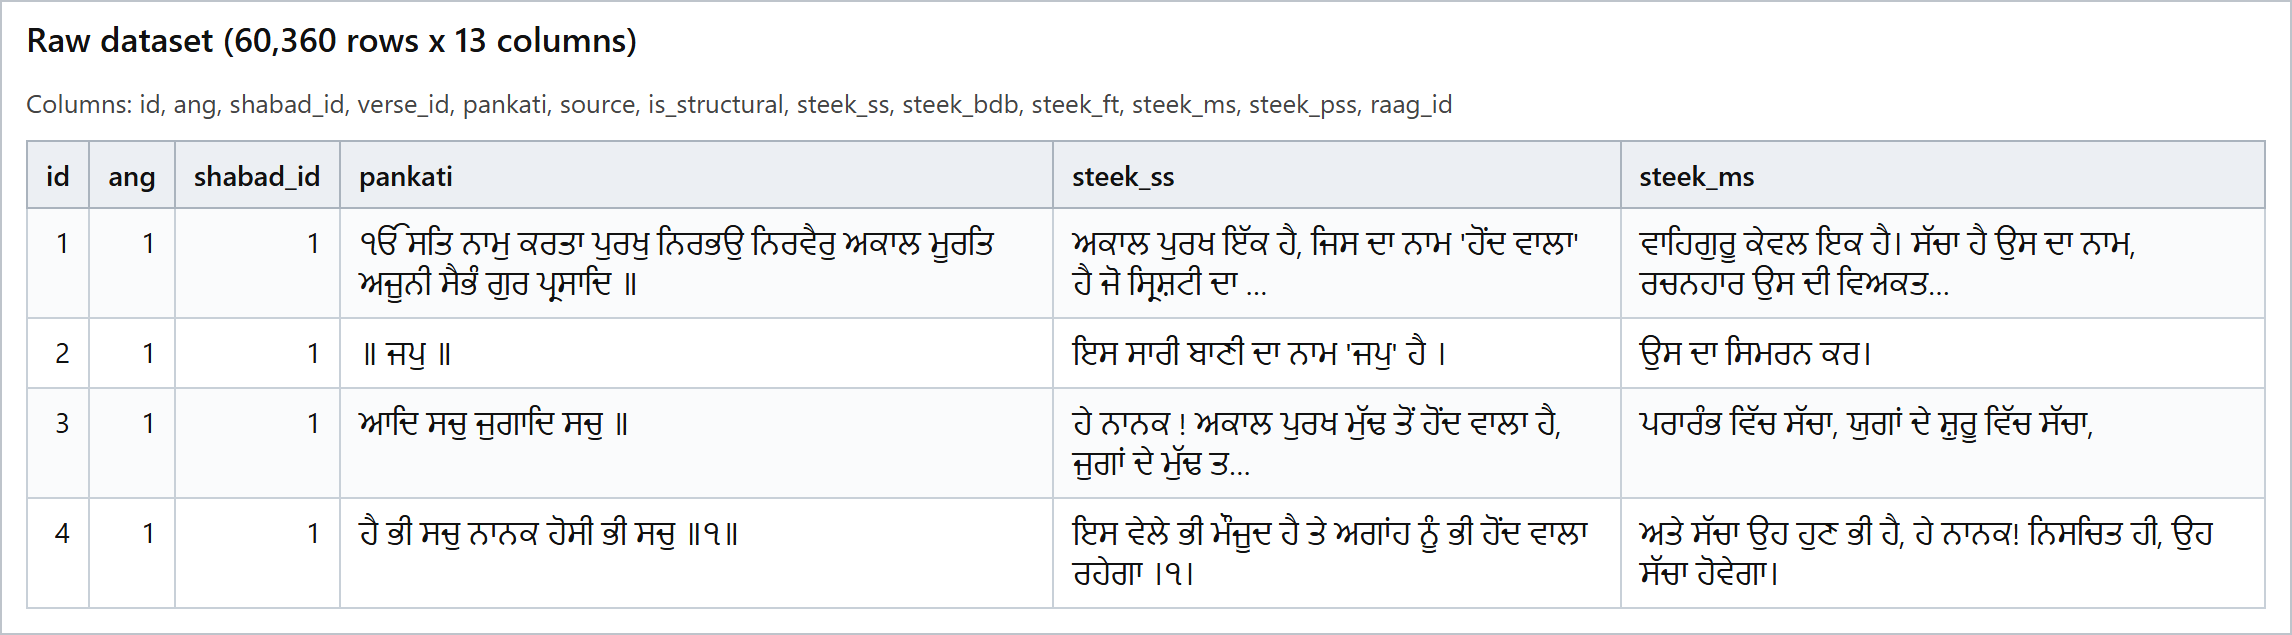
\includegraphics[width=\textwidth]{fig_dataset_raw.png}
\caption{Structure of the raw dataset with Pankatis and their commentaries}
\label{fig:auto12}
\end{figure}


\begin{figure}[H]
\centering
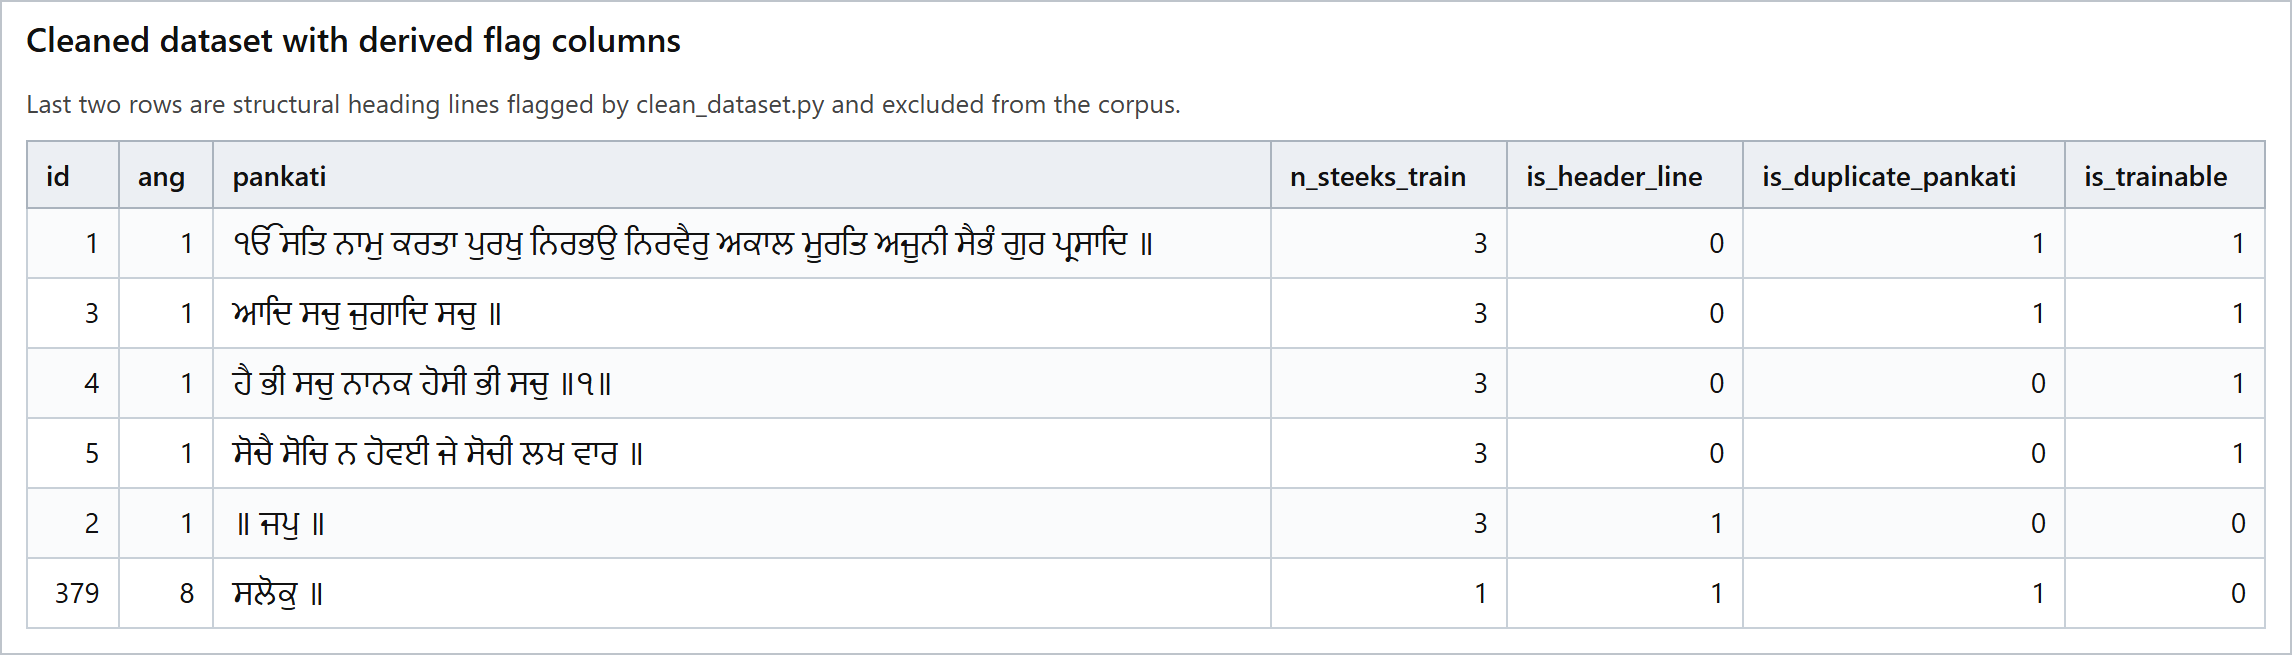
\includegraphics[width=\textwidth]{fig_dataset_cleaned.png}
\caption{Cleaned dataset showing the derived flag columns; the final two rows are structural heading lines}
\label{fig:auto13}
\end{figure}


\begin{figure}[H]
\centering
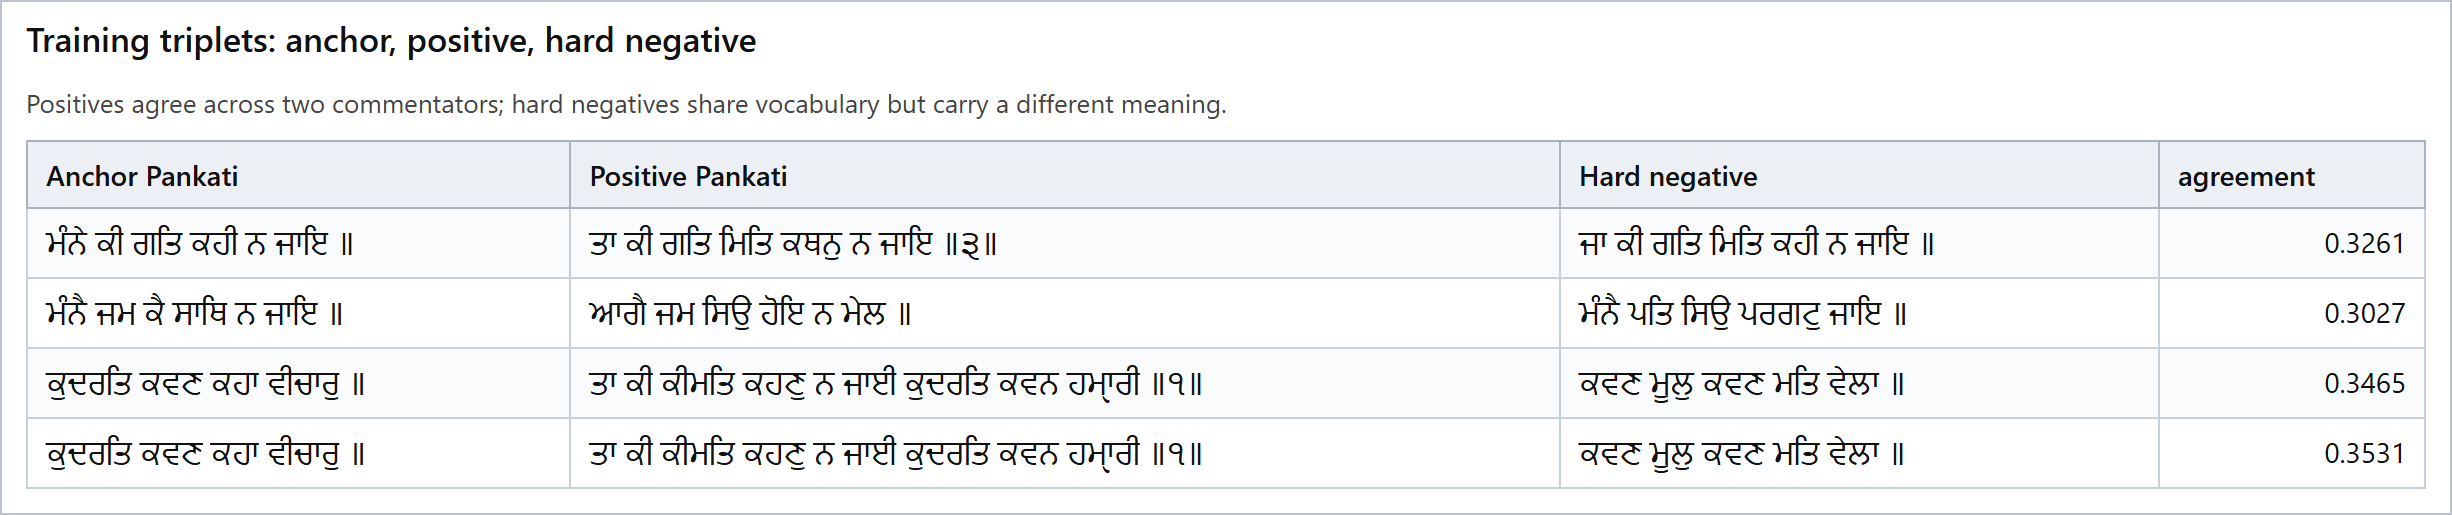
\includegraphics[width=\textwidth]{fig_training_pairs.png}
\caption{Mined training triplets of anchor, positive and hard negative}
\label{fig:auto14}
\end{figure}


\begin{figure}[H]
\centering
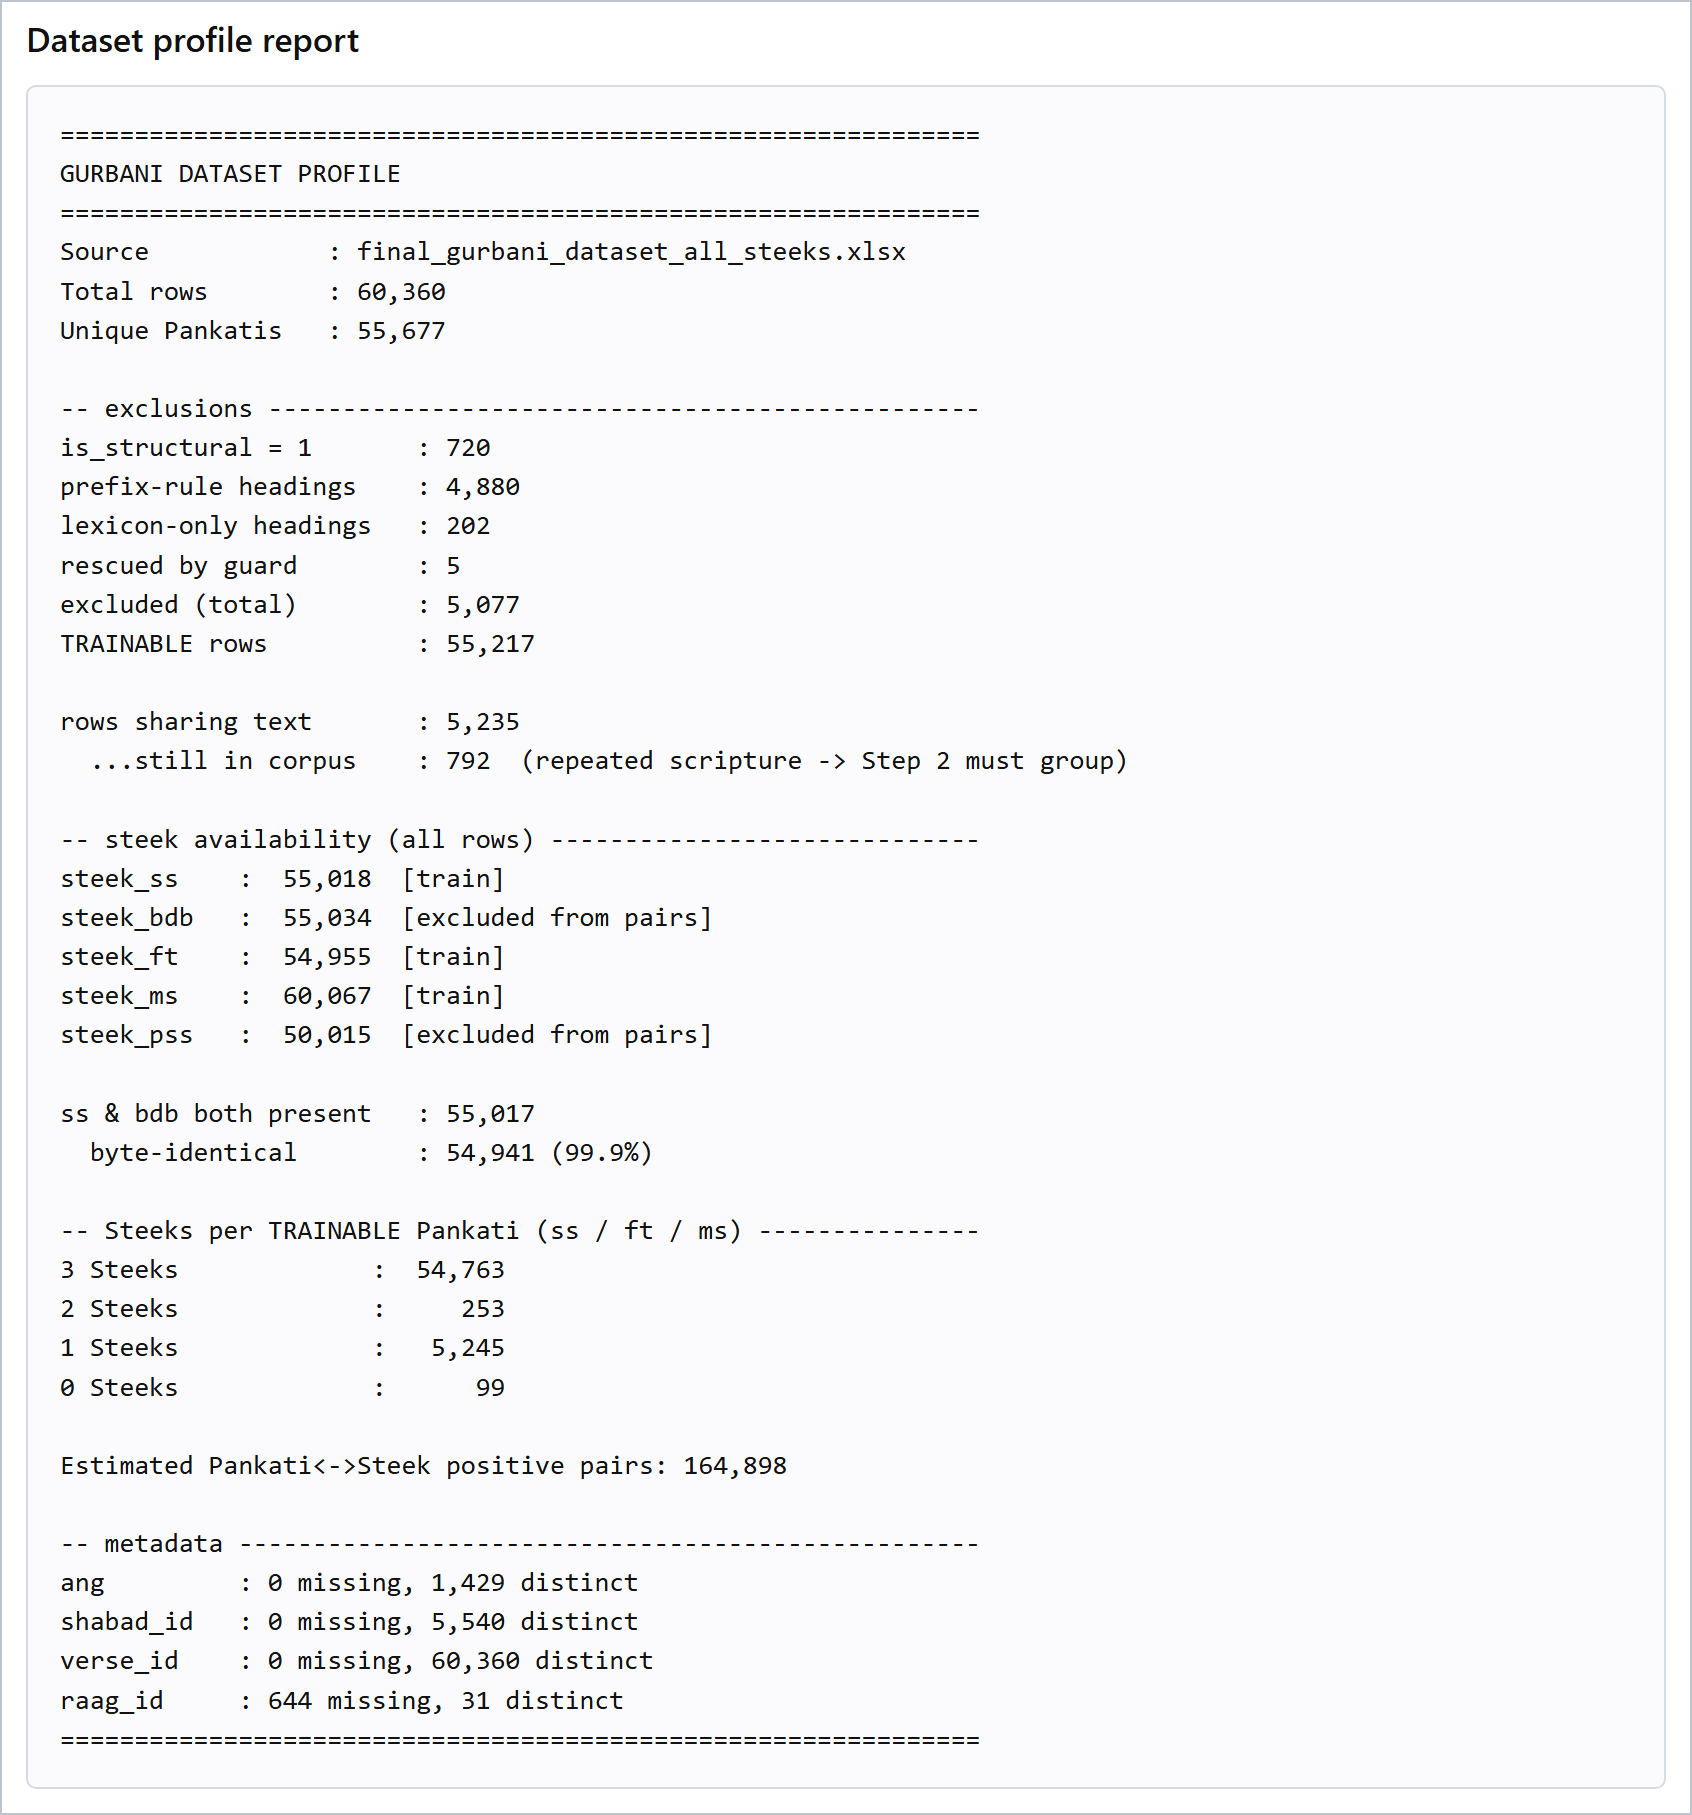
\includegraphics[width=0.86\textwidth]{fig_profile_report.png}
\caption{Dataset profile report produced by the preprocessing module}
\label{fig:auto15}
\end{figure}


\begin{figure}[H]
\centering
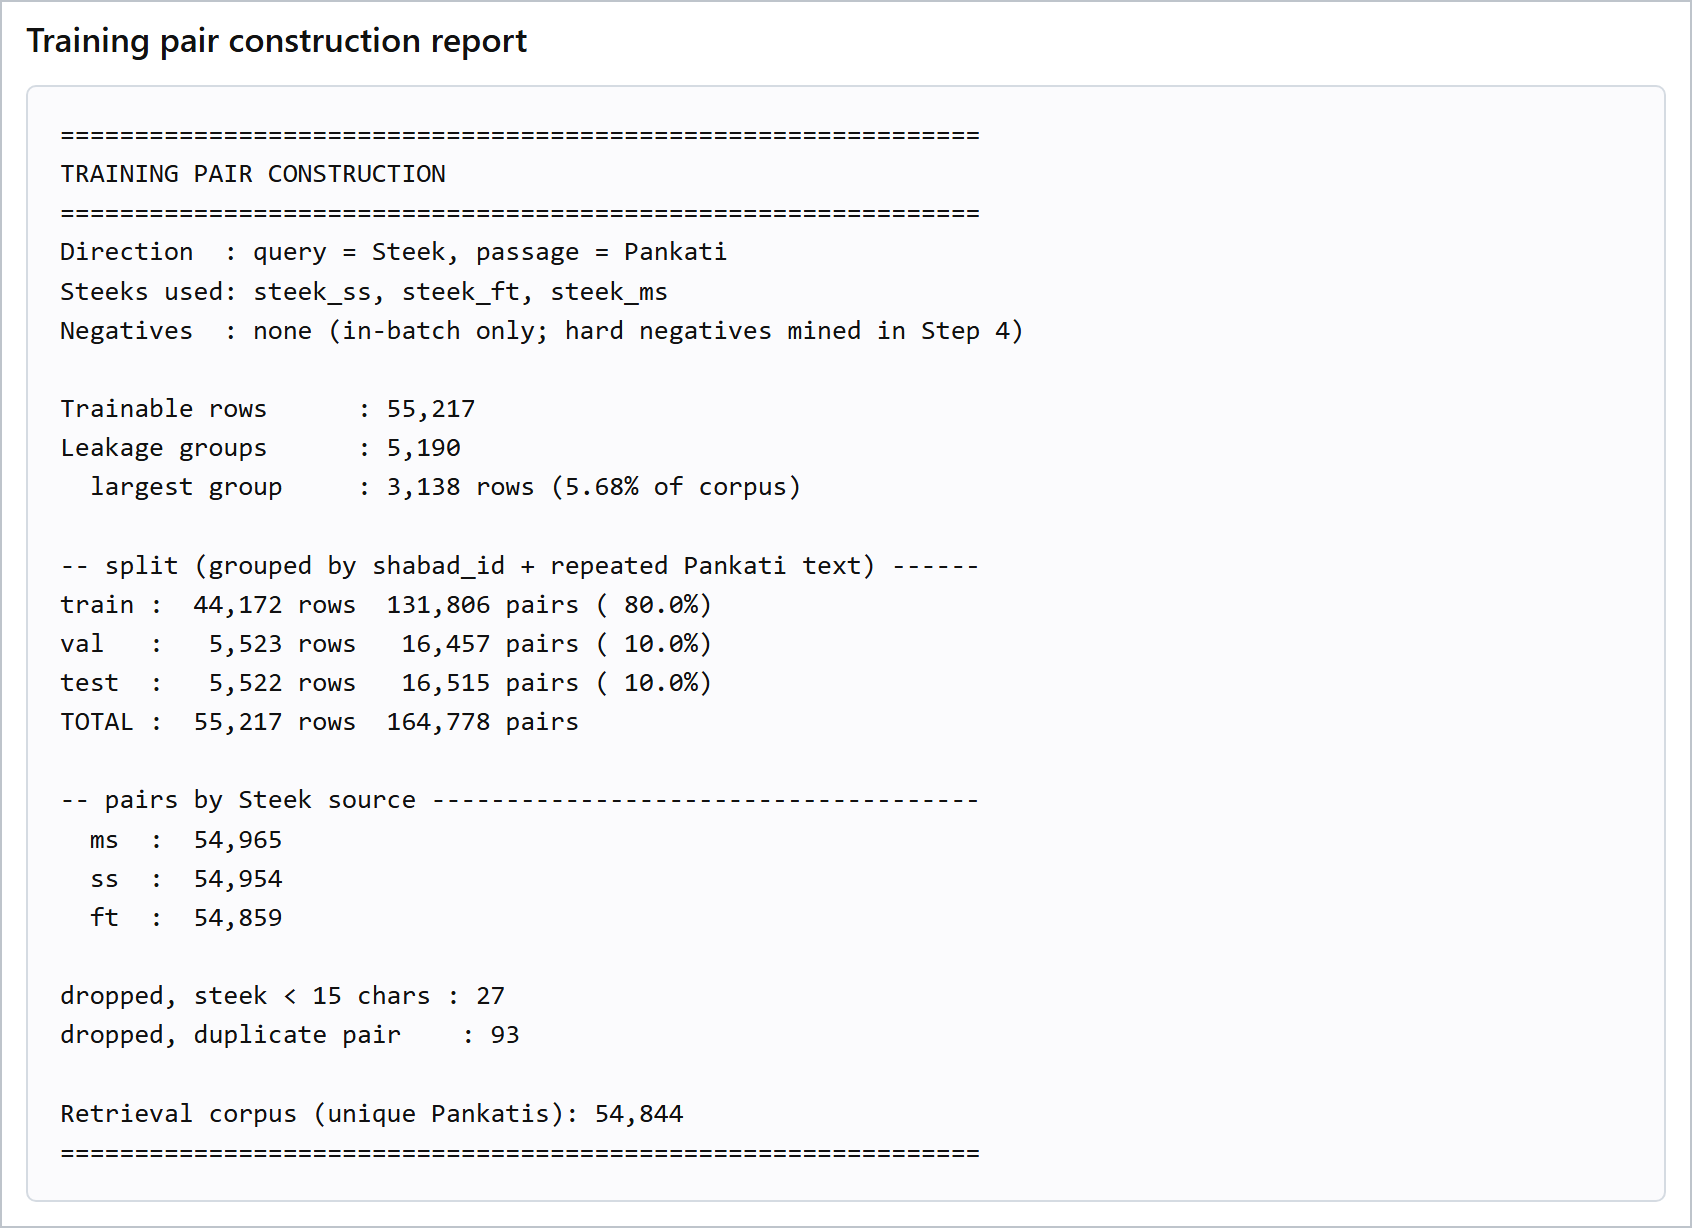
\includegraphics[width=0.86\textwidth]{fig_pairs_report.png}
\caption{Training pair construction report showing the leakage-free partition}
\label{fig:auto16}
\end{figure}


\begin{figure}[H]
\centering
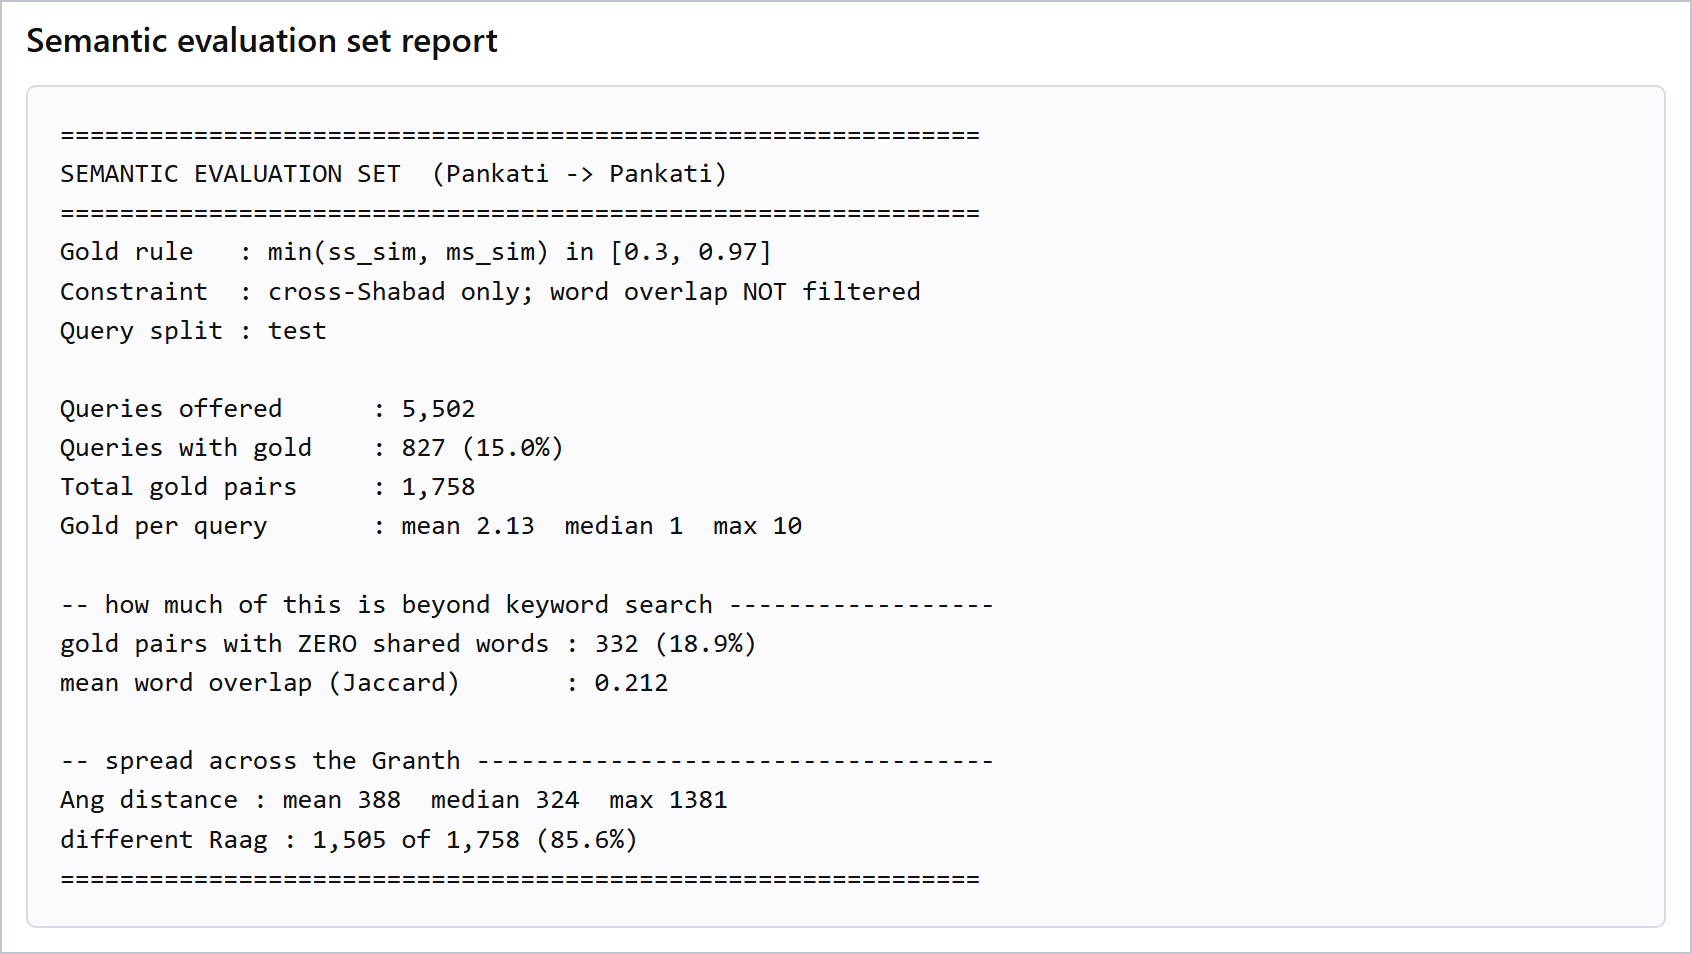
\includegraphics[width=0.86\textwidth]{fig_eval_report.png}
\caption{Report of the mined evaluation benchmark}
\label{fig:auto17}
\end{figure}


\begin{figure}[H]
\centering
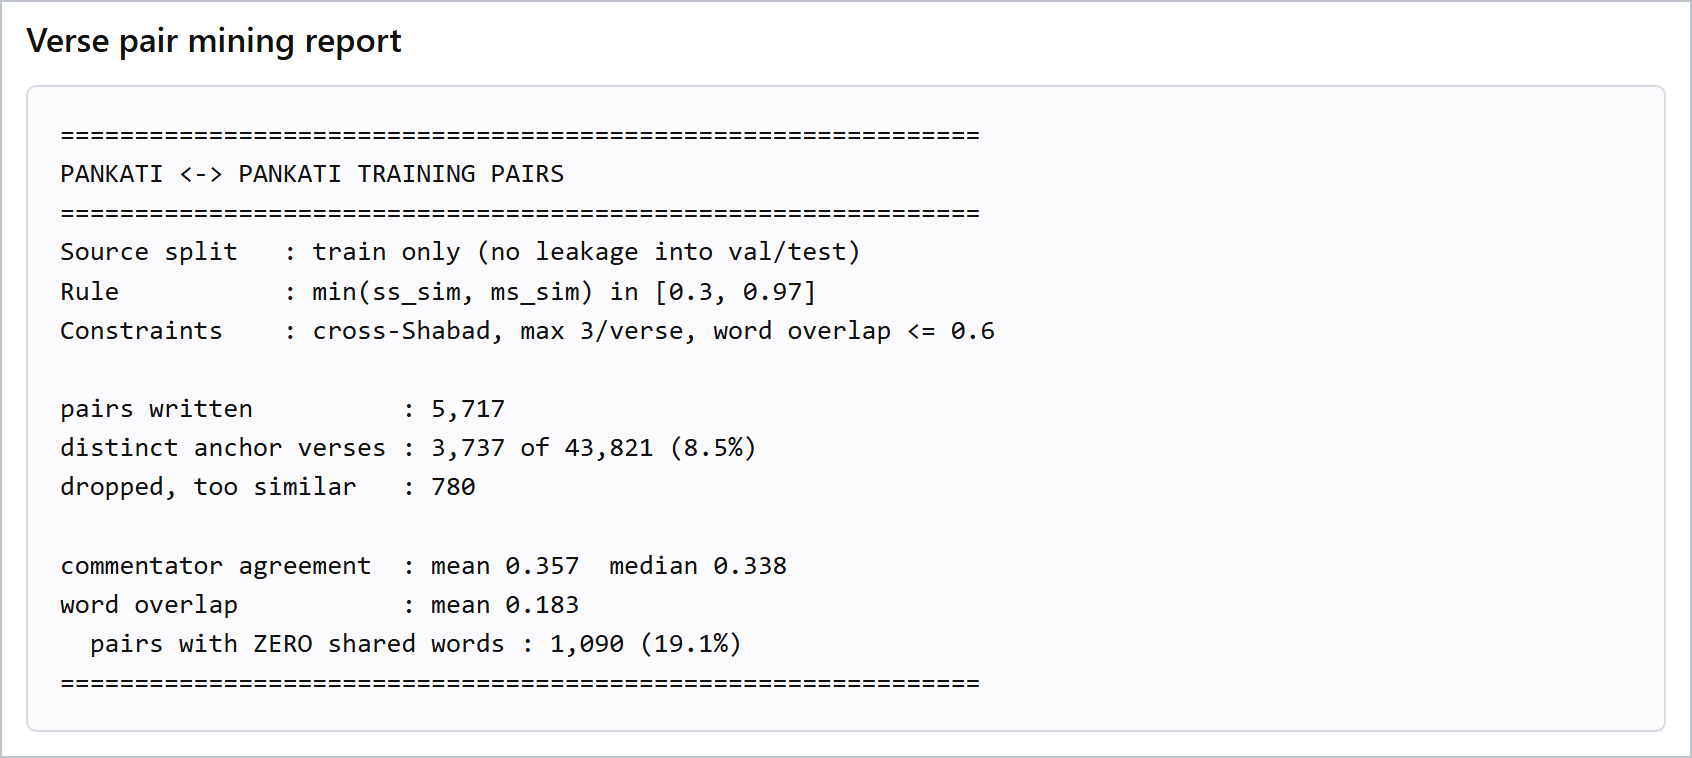
\includegraphics[width=0.86\textwidth]{fig_versepairs_report.png}
\caption{Report of the mined Pankati-to-Pankati training pairs}
\label{fig:auto18}
\end{figure}


\begin{figure}[H]
\centering
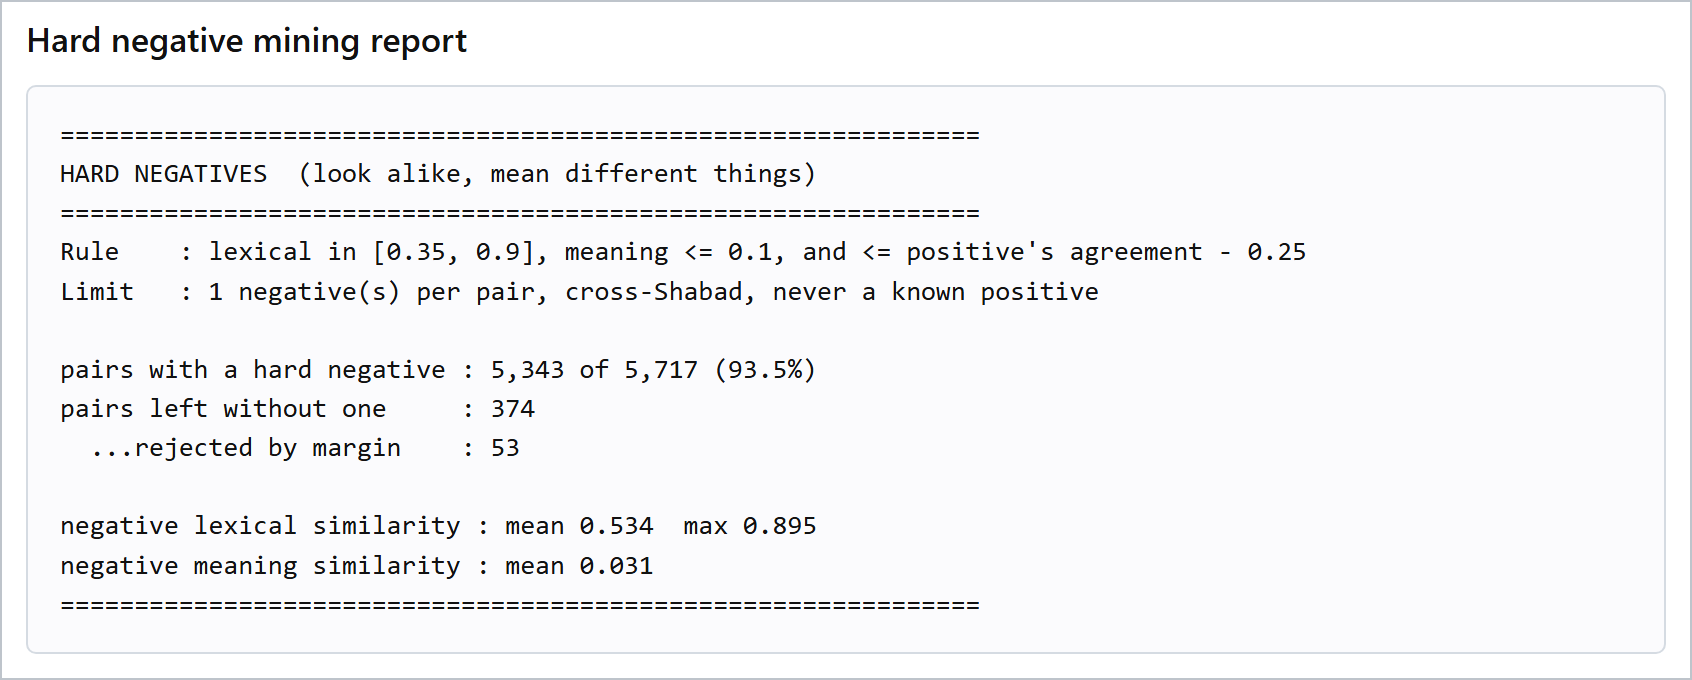
\includegraphics[width=0.86\textwidth]{fig_hn_report.png}
\caption{Report of the mined hard negatives}
\label{fig:auto19}
\end{figure}


\begin{figure}[H]
\centering
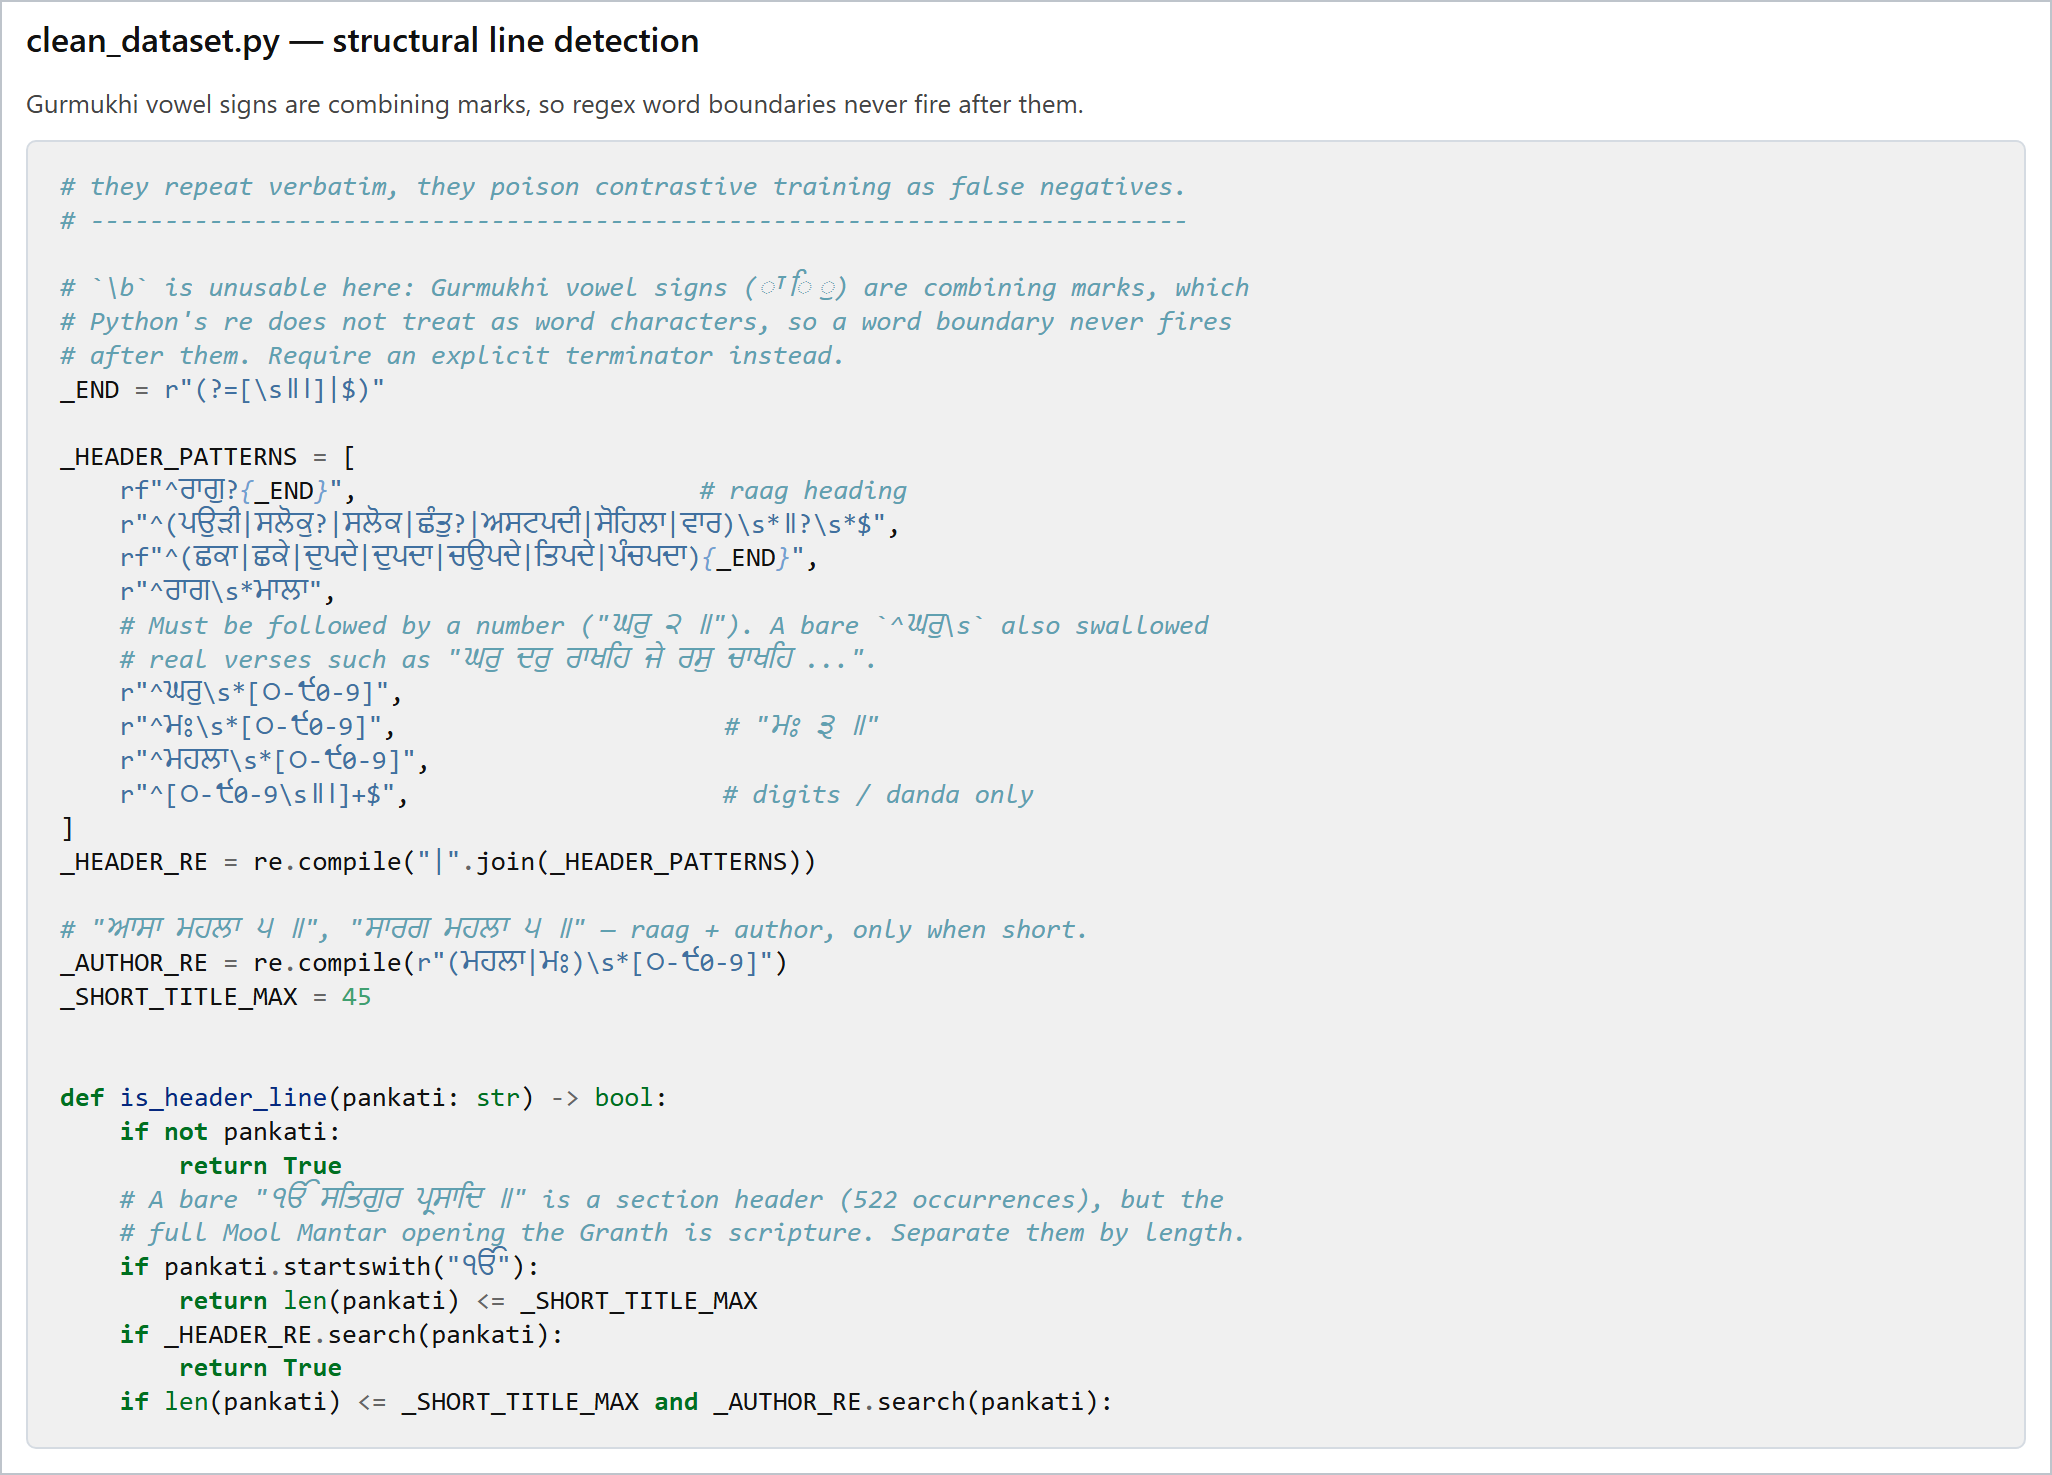
\includegraphics[width=0.92\textwidth]{fig_code_clean.png}
\caption{Implementation of the structural line detector}
\label{fig:auto20}
\end{figure}


\begin{figure}[H]
\centering
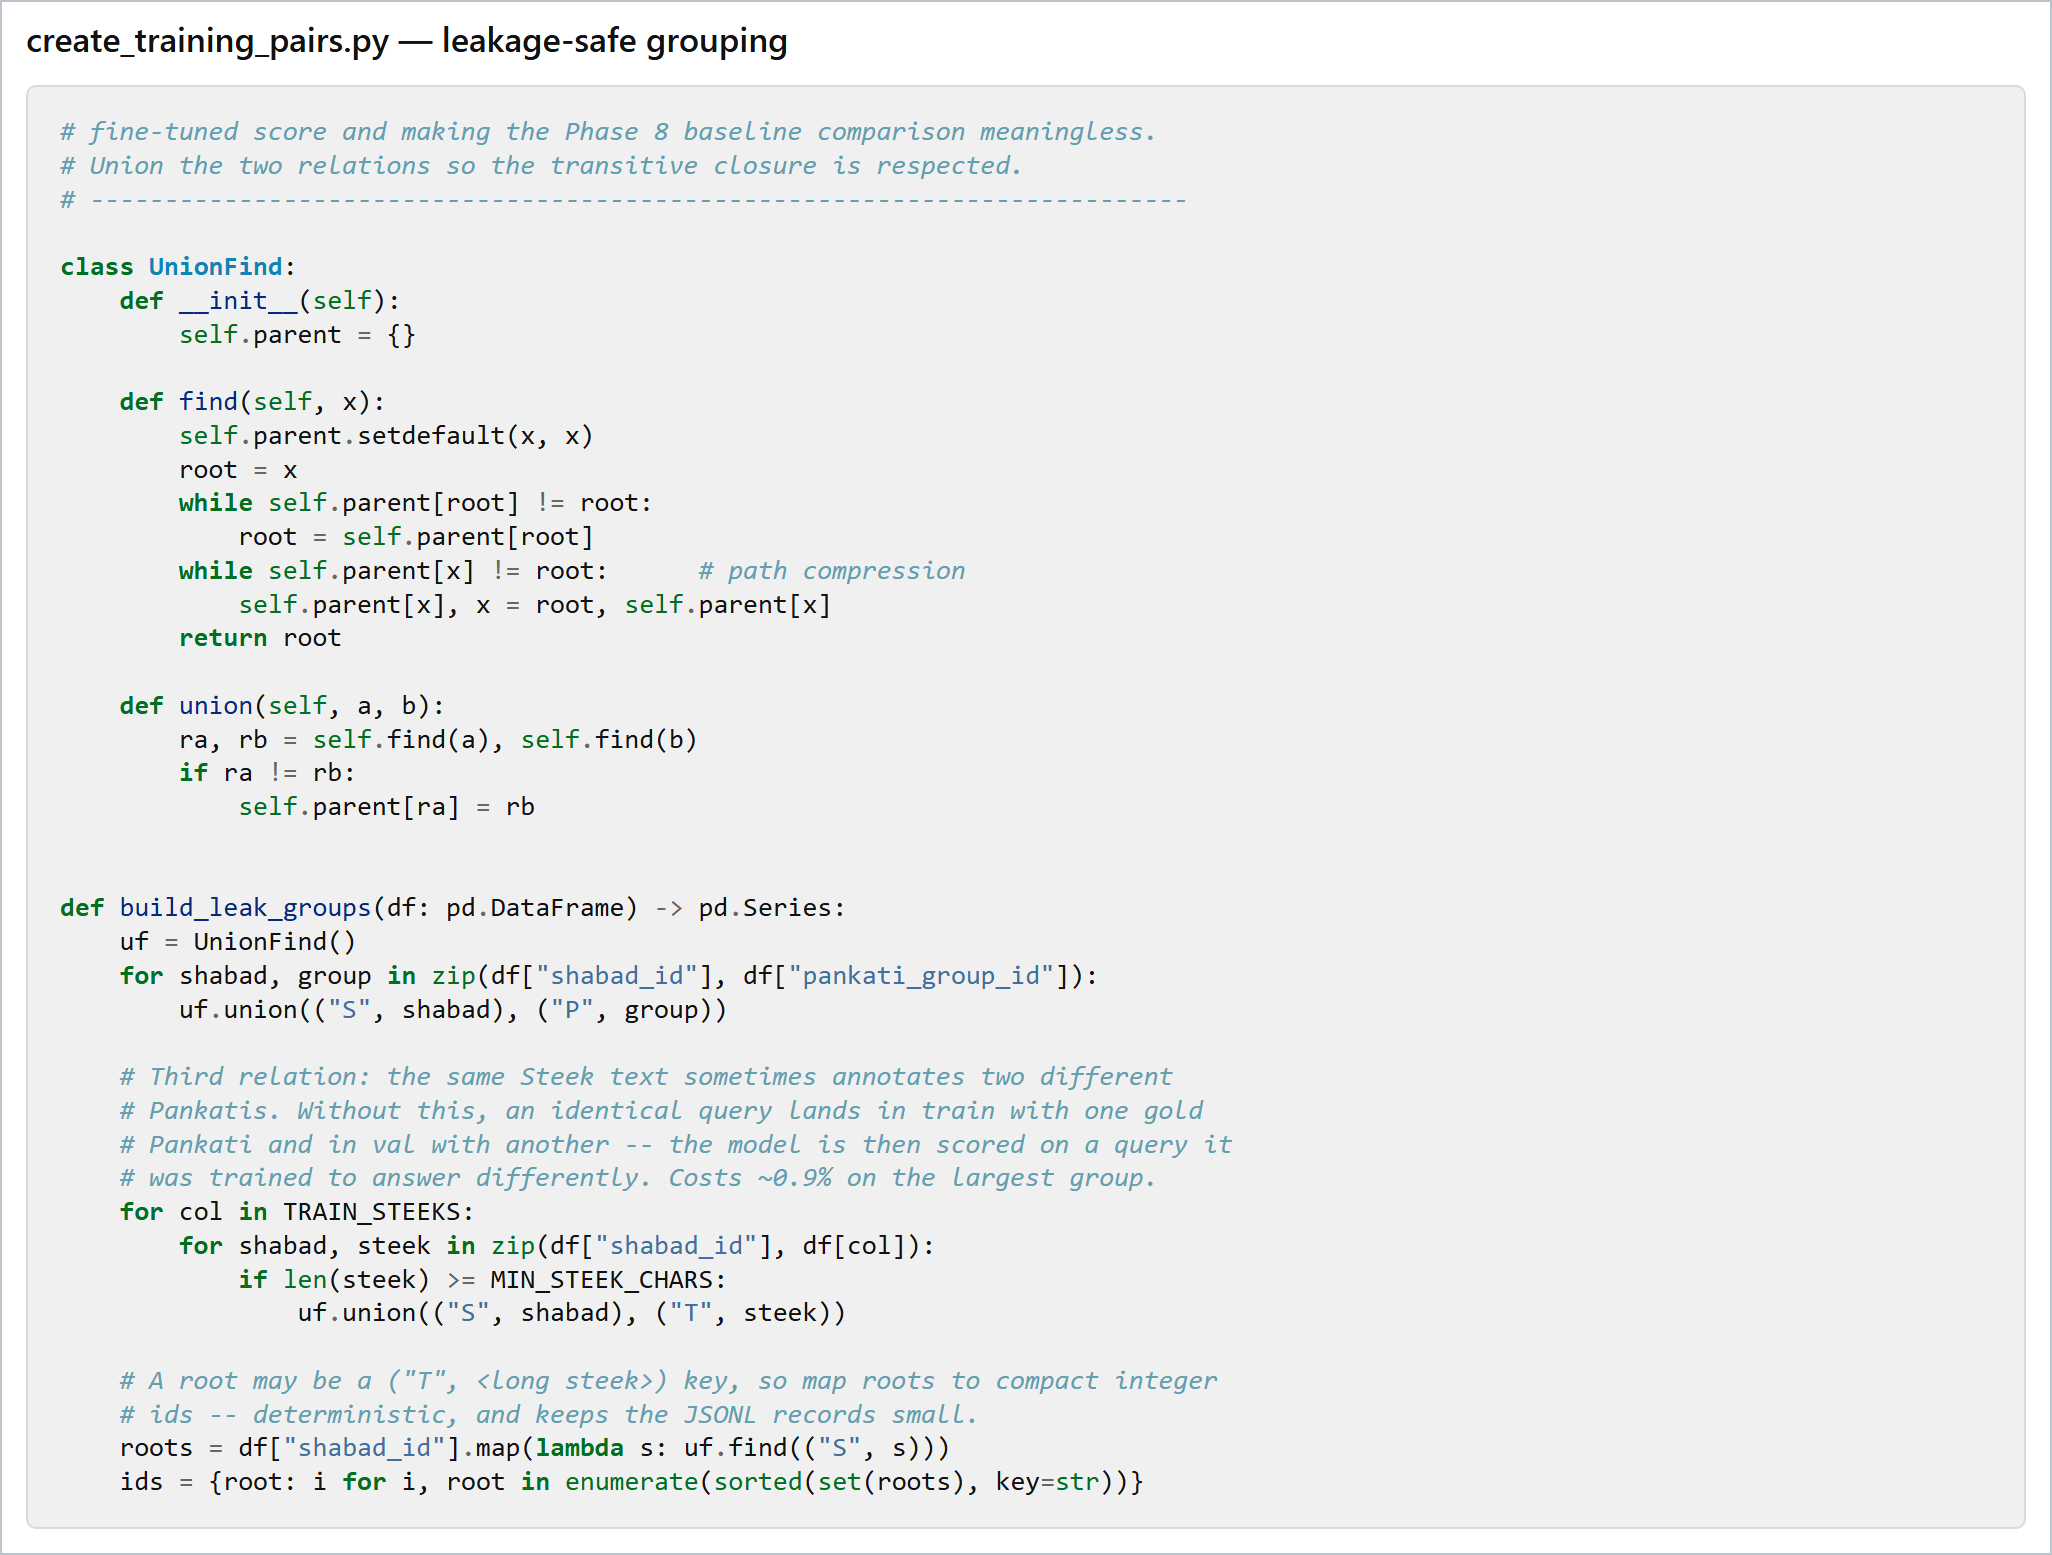
\includegraphics[width=0.92\textwidth]{fig_code_pairs.png}
\caption{Implementation of the leakage-free partitioning procedure}
\label{fig:auto21}
\end{figure}


\begin{figure}[H]
\centering
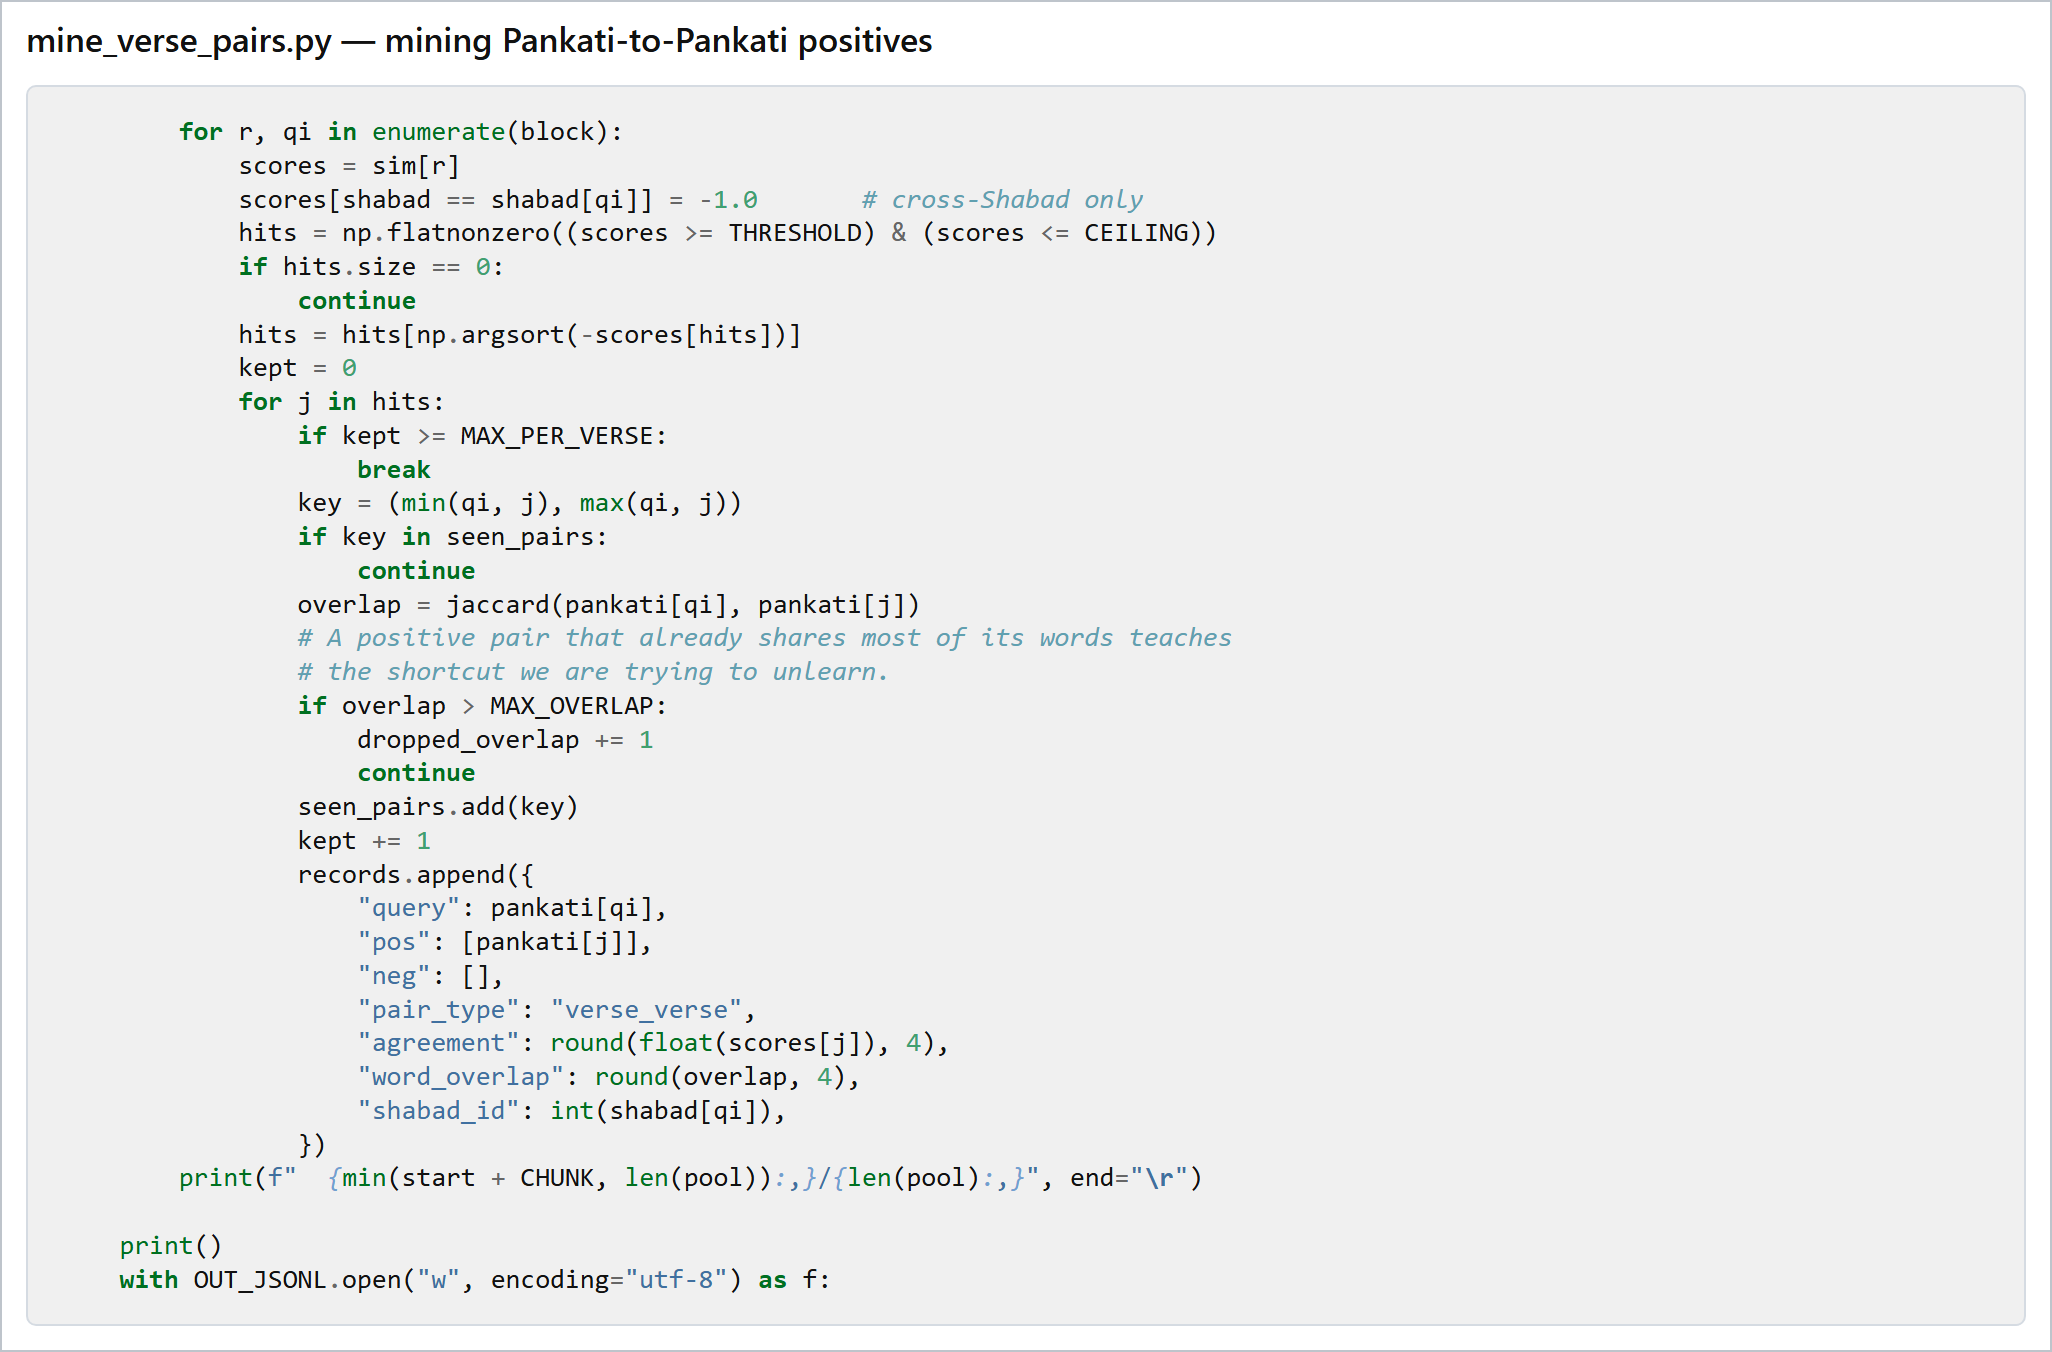
\includegraphics[width=0.92\textwidth]{fig_code_mine.png}
\caption{Implementation of the Pankati-to-Pankati pair mining}
\label{fig:auto22}
\end{figure}


\begin{figure}[H]
\centering
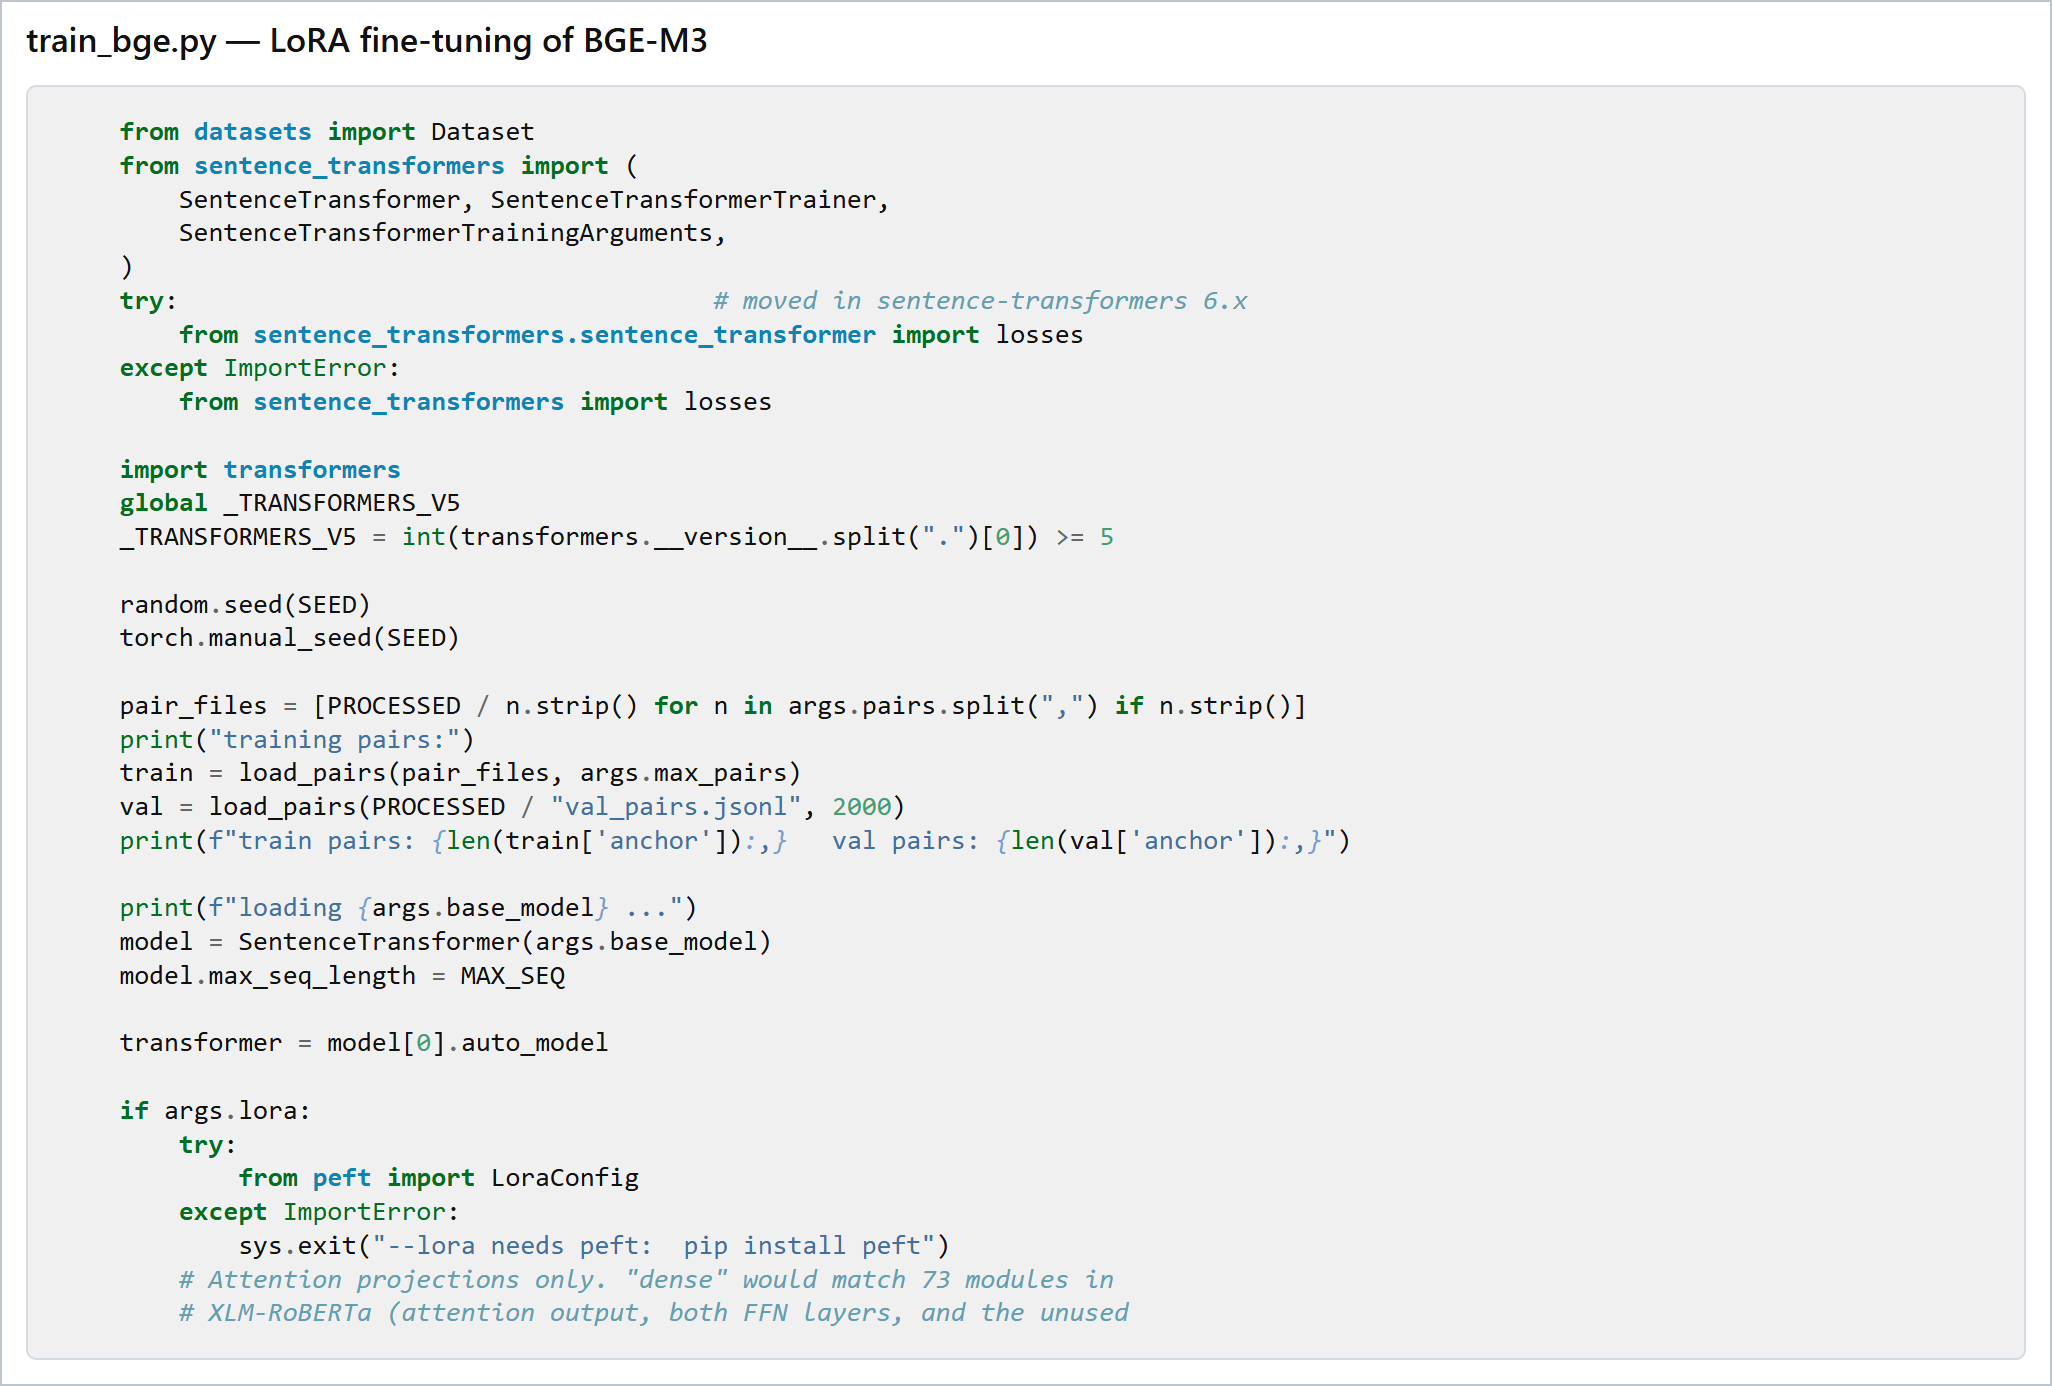
\includegraphics[width=0.92\textwidth]{fig_code_train.png}
\caption{Implementation of the LoRA fine-tuning procedure}
\label{fig:auto23}
\end{figure}

% ===================== OUTPUT SCREENS =====================
\newpage
\section{Output Screens}
\addcontentsline{toc}{section}{Output Screens}

This chapter presents the output of the working retrieval system. The interface is at present a command-line application; the graphical user interface described in the synopsis is scheduled for the remaining phase of the project.

\subsection{Retrieval Output}


\begin{figure}[H]
\centering
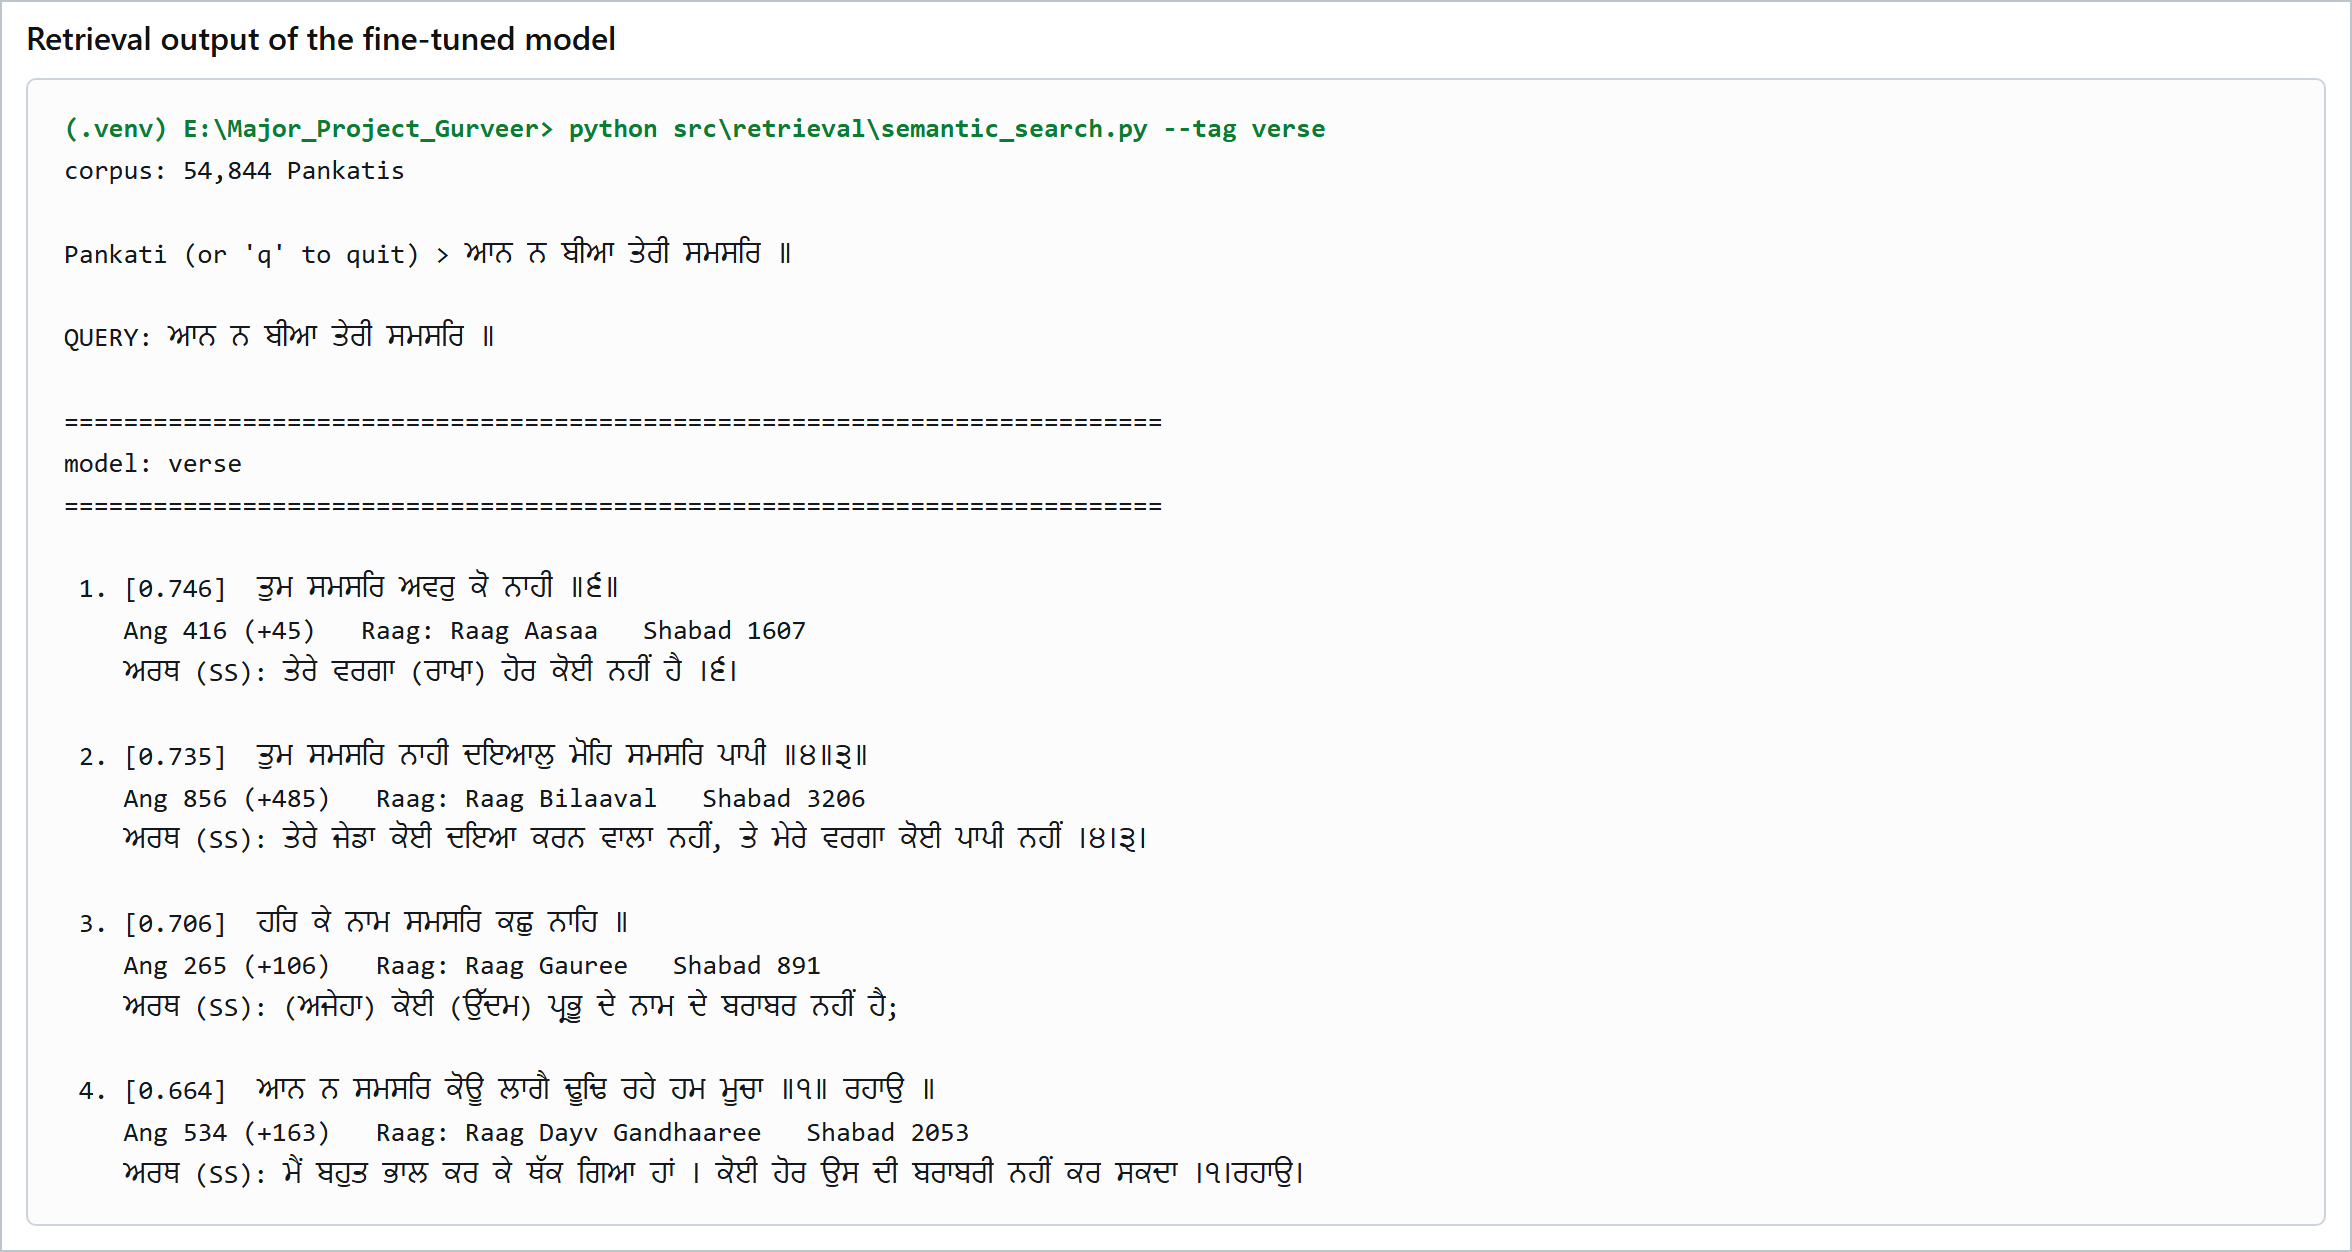
\includegraphics[width=\textwidth]{fig_output_search.png}
\caption{Retrieval output for a query Pankati, showing similarity score, Ang, Raag, Shabad and Steek for each result}
\label{fig:auto24}
\end{figure}

\subsection{Comparison of the Pretrained and Fine-tuned Models}


\begin{figure}[H]
\centering
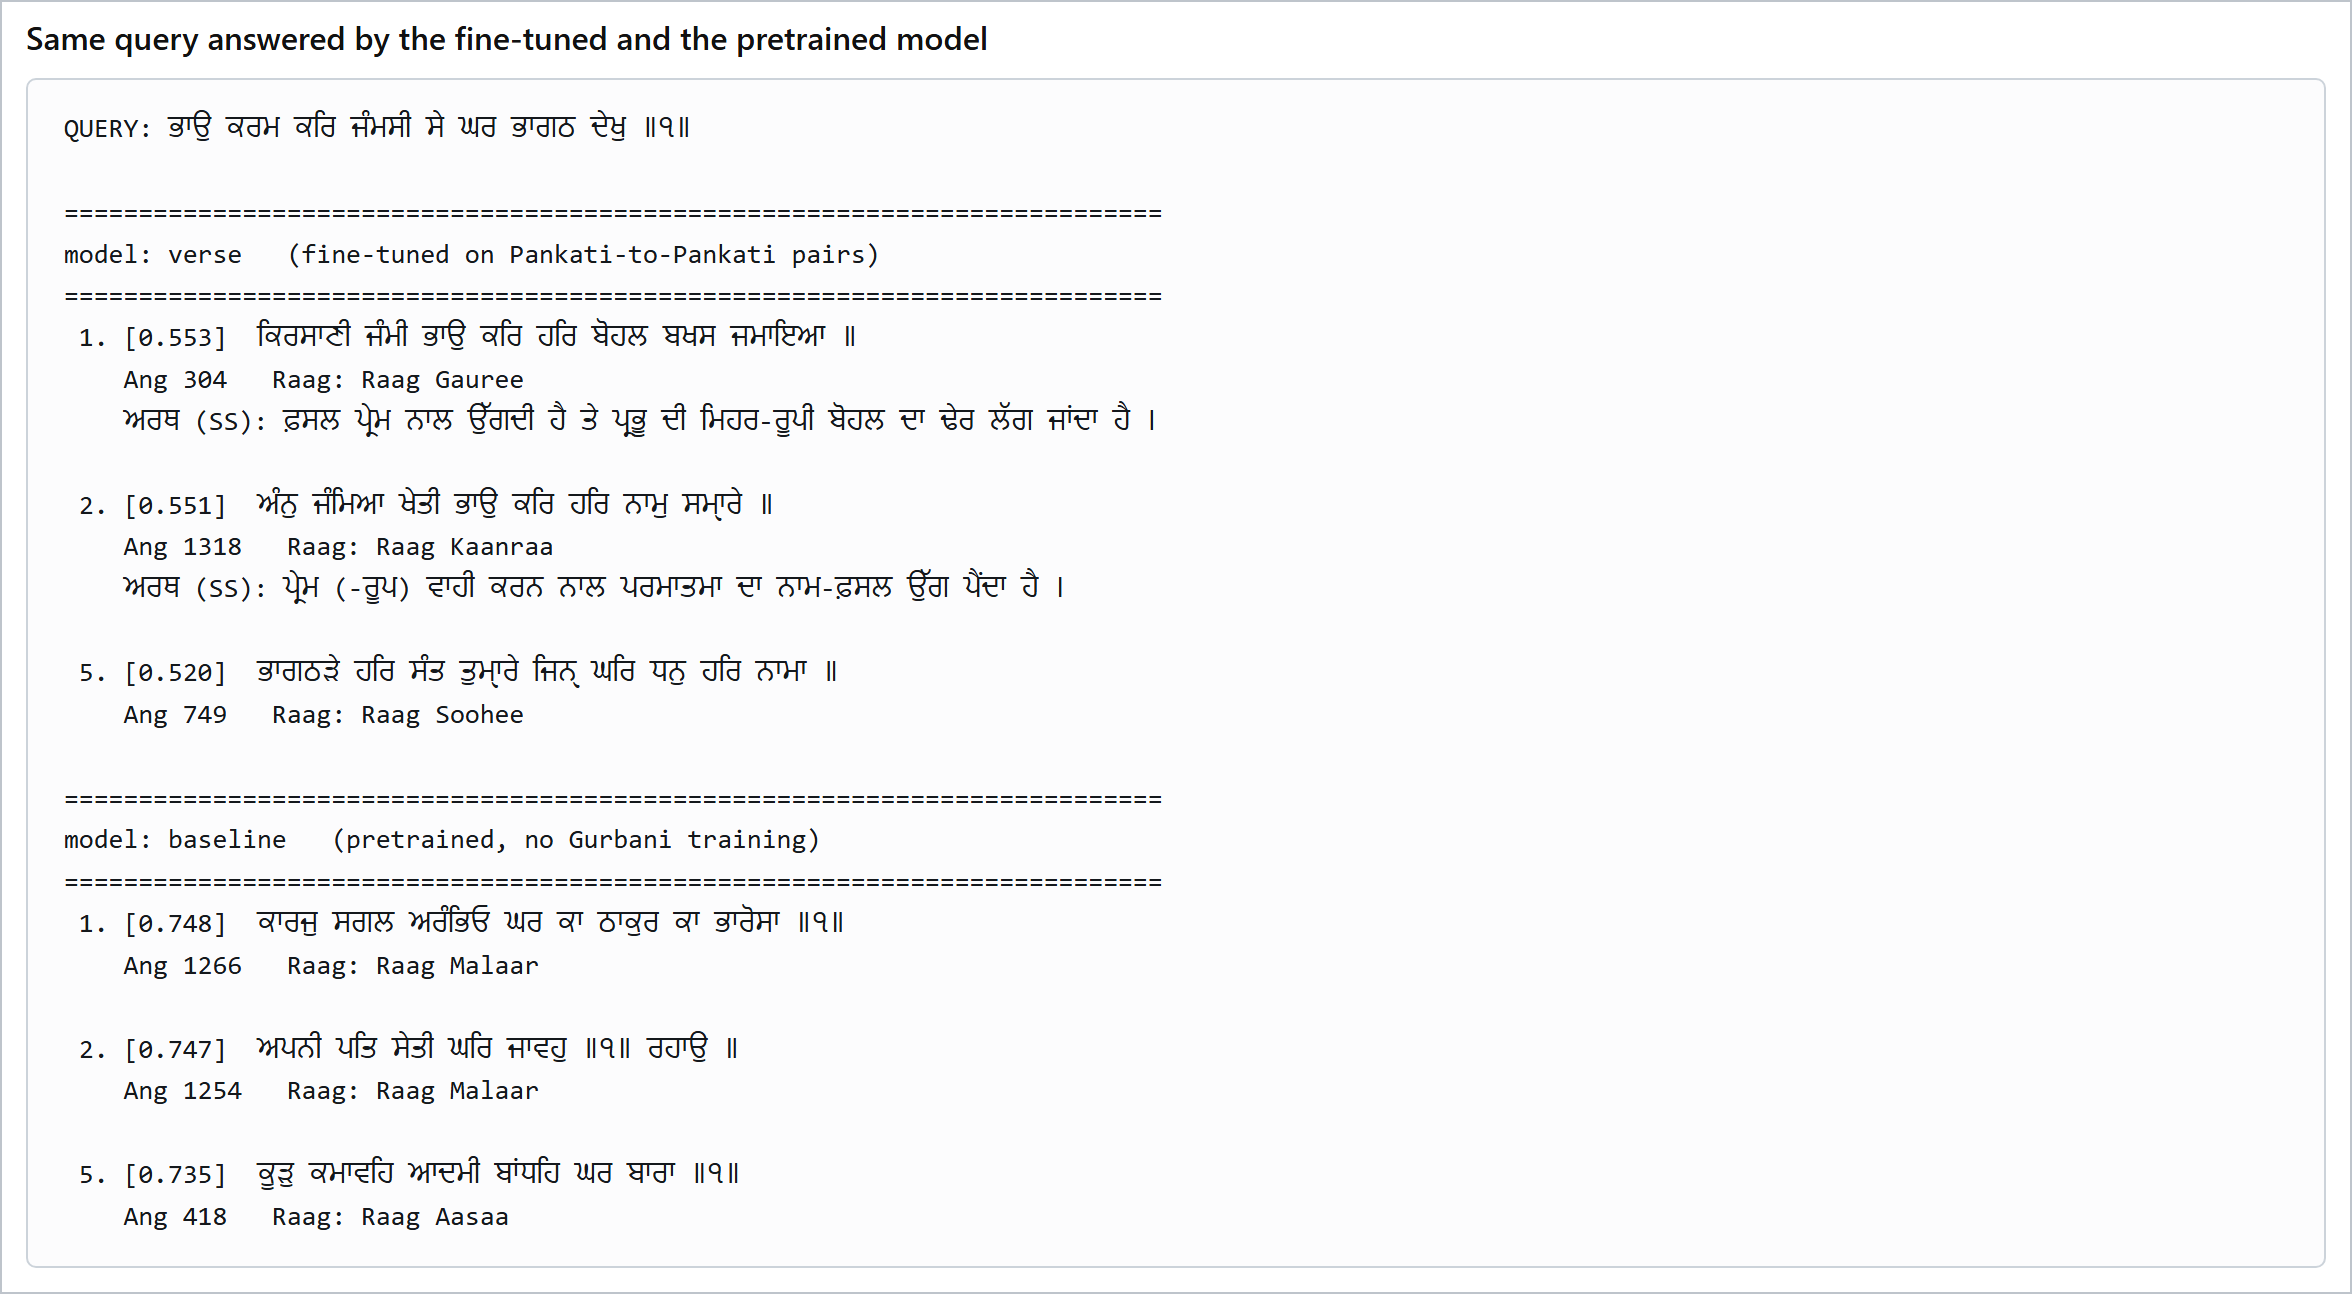
\includegraphics[width=\textwidth]{fig_output_compare.png}
\caption{Side-by-side output of the pretrained and fine-tuned models for the same query}
\label{fig:auto25}
\end{figure}

\subsection{Training Output}


\begin{figure}[H]
\centering
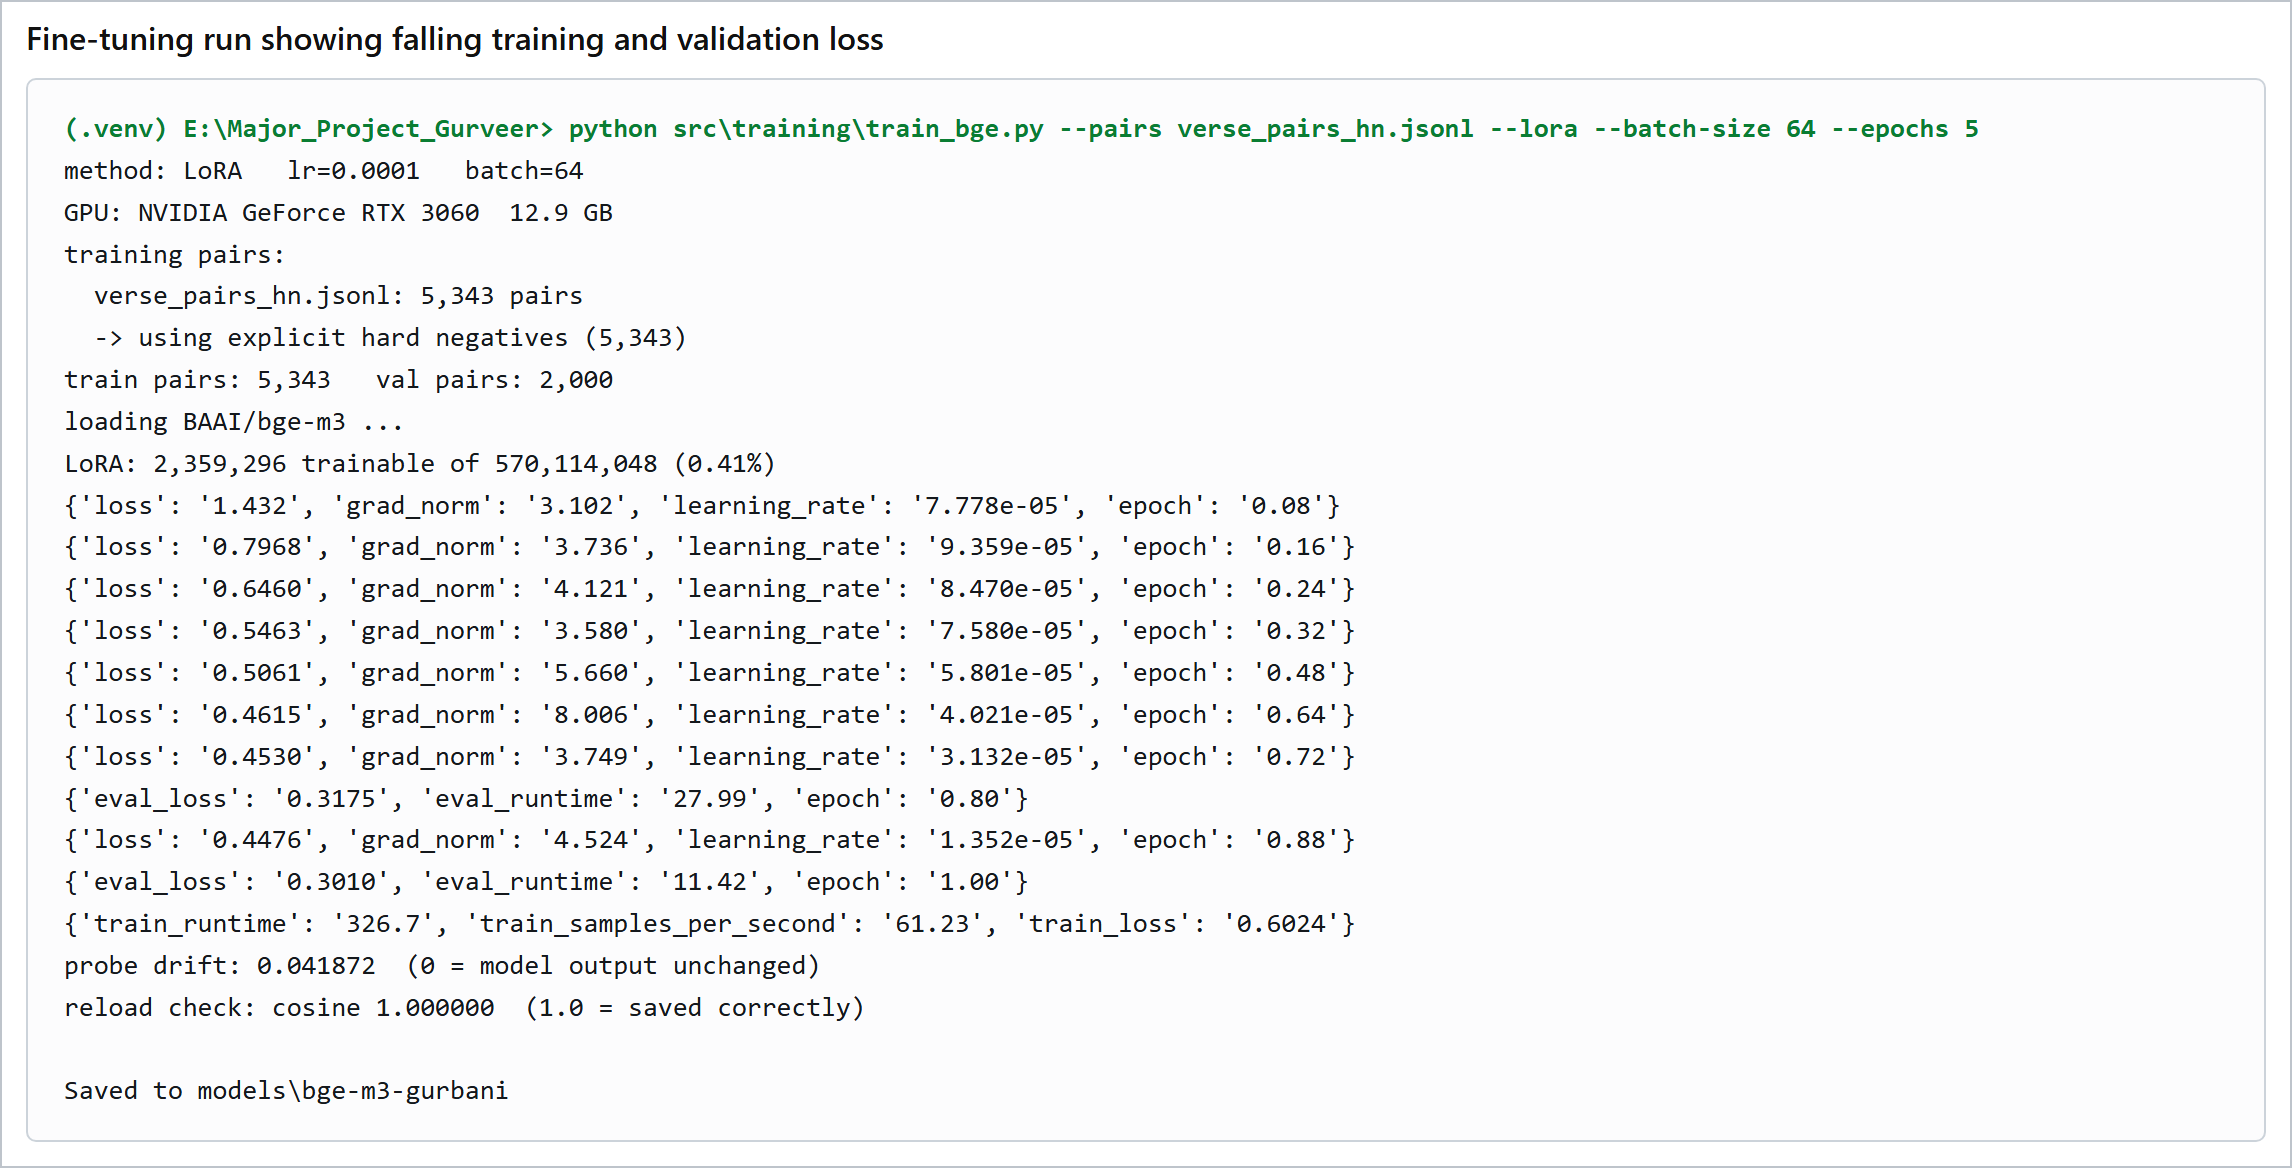
\includegraphics[width=\textwidth]{fig_output_training.png}
\caption{Fine-tuning run showing the falling training and validation loss}
\label{fig:auto26}
\end{figure}

\subsection{Evaluation Output}


\begin{figure}[H]
\centering
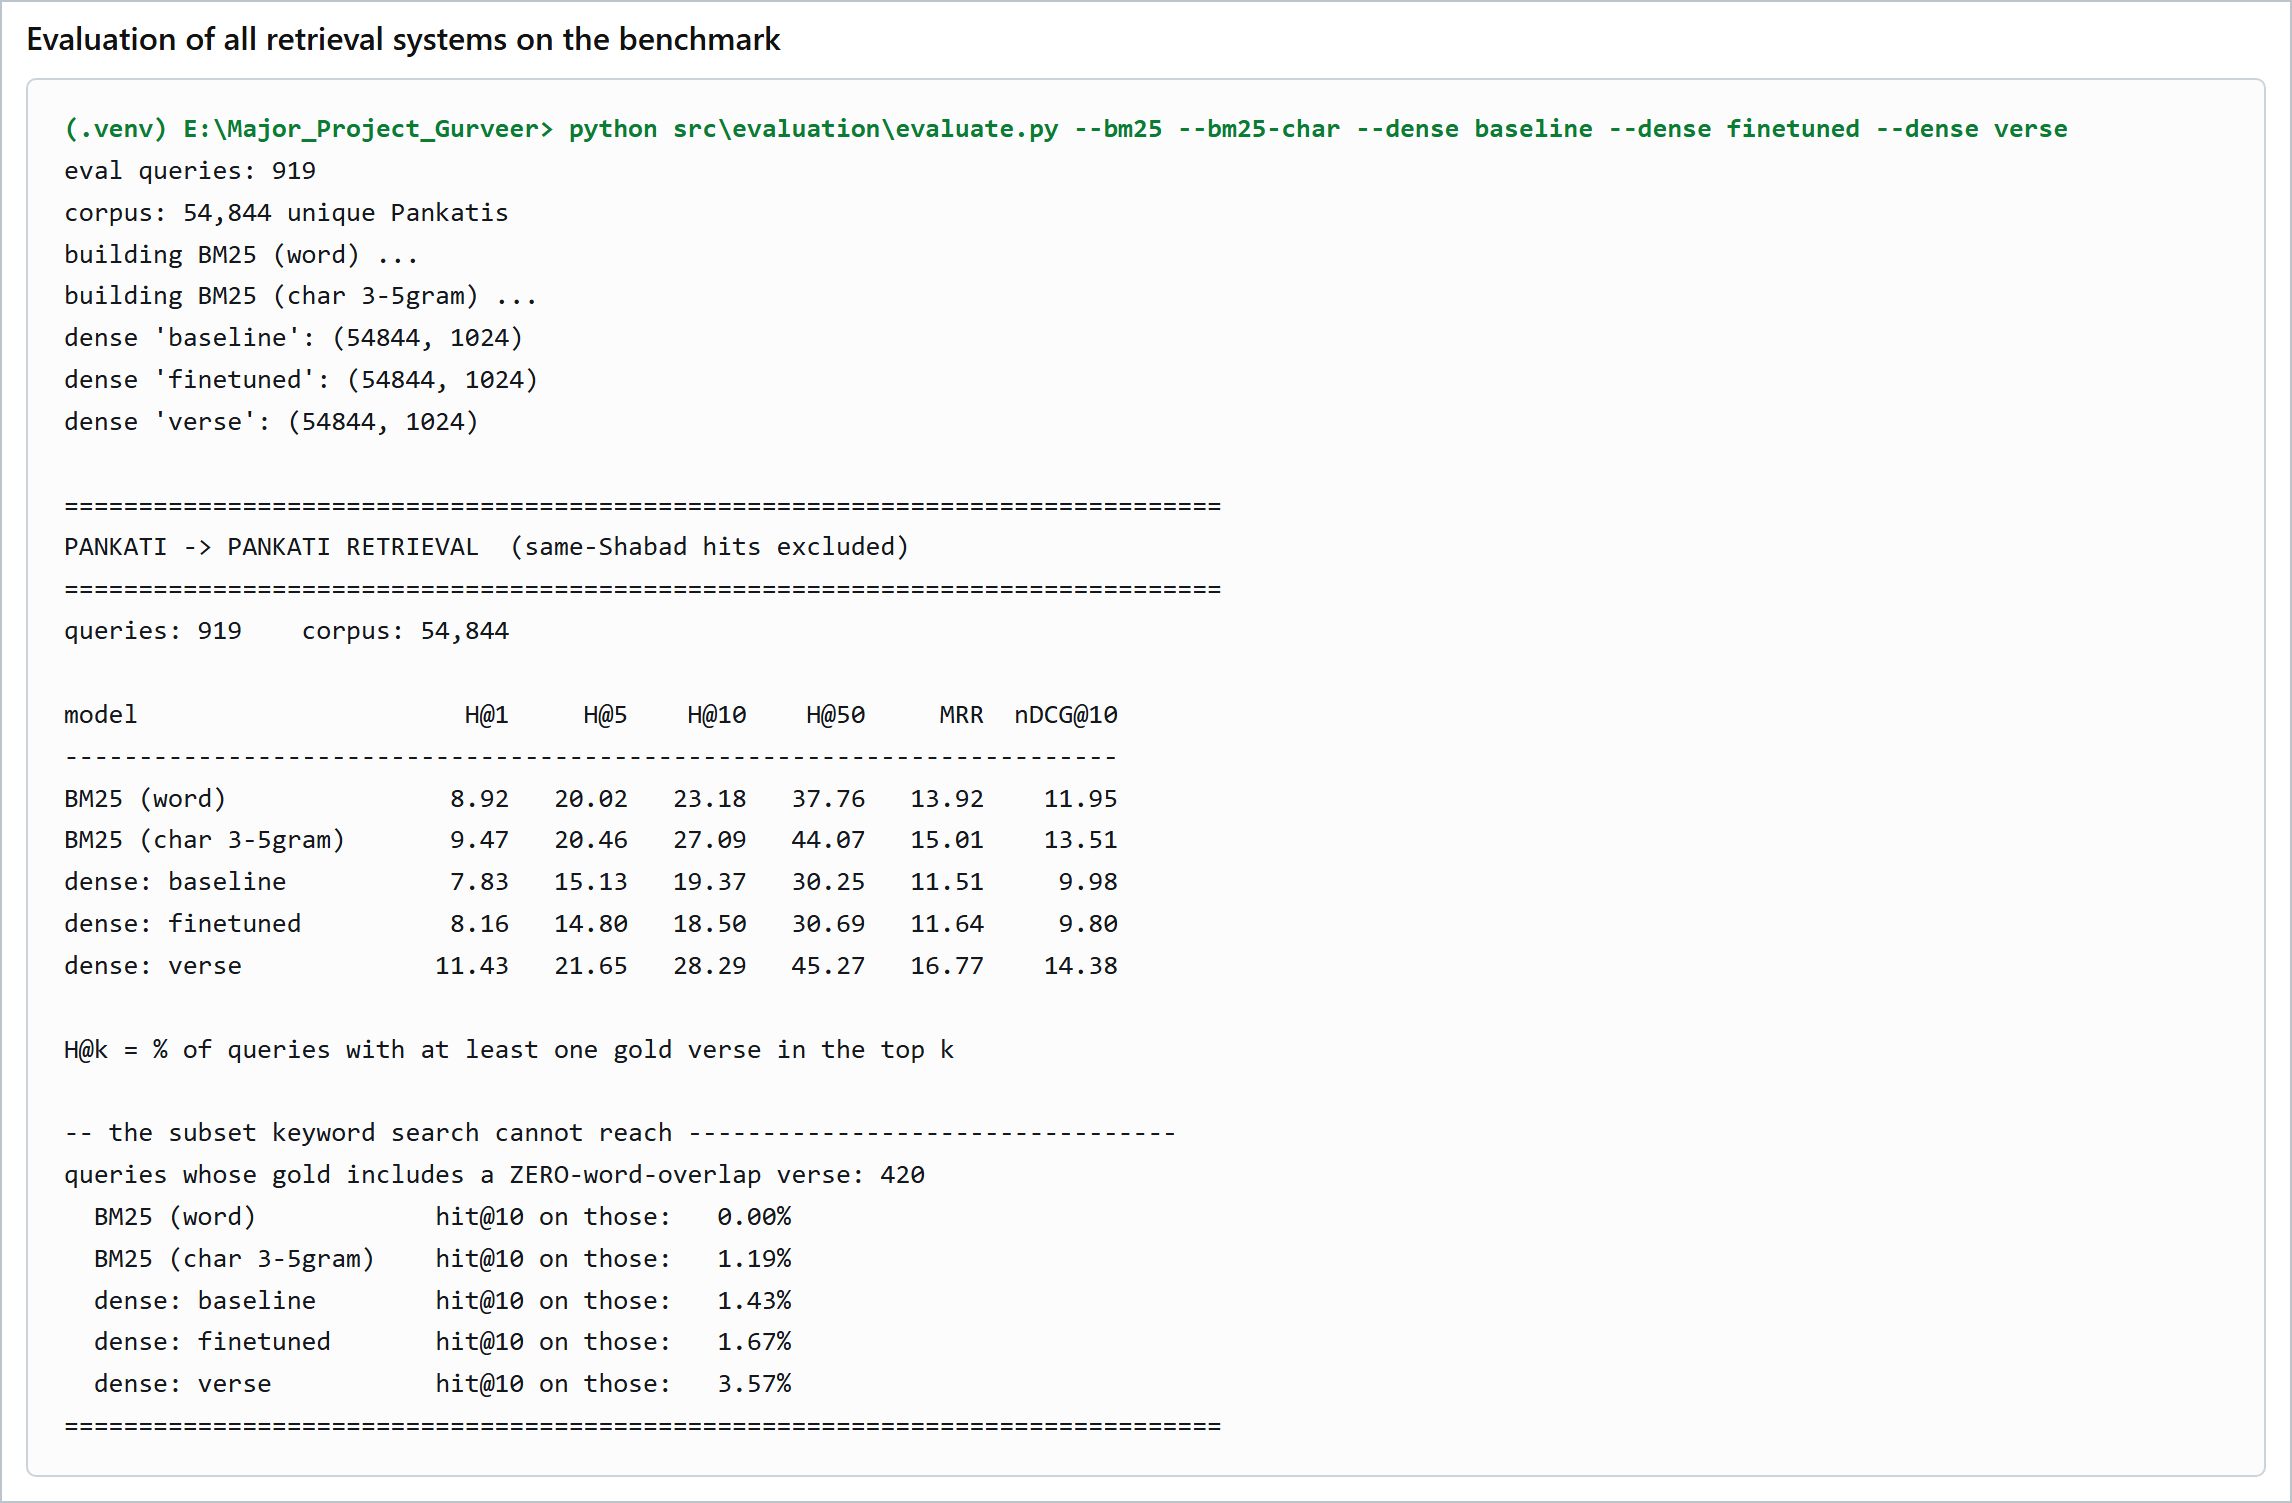
\includegraphics[width=\textwidth]{fig_output_evaluate.png}
\caption{Evaluation output comparing all retrieval systems on the benchmark}
\label{fig:auto27}
\end{figure}

\subsection{Corpus Encoding Output}


\begin{figure}[H]
\centering
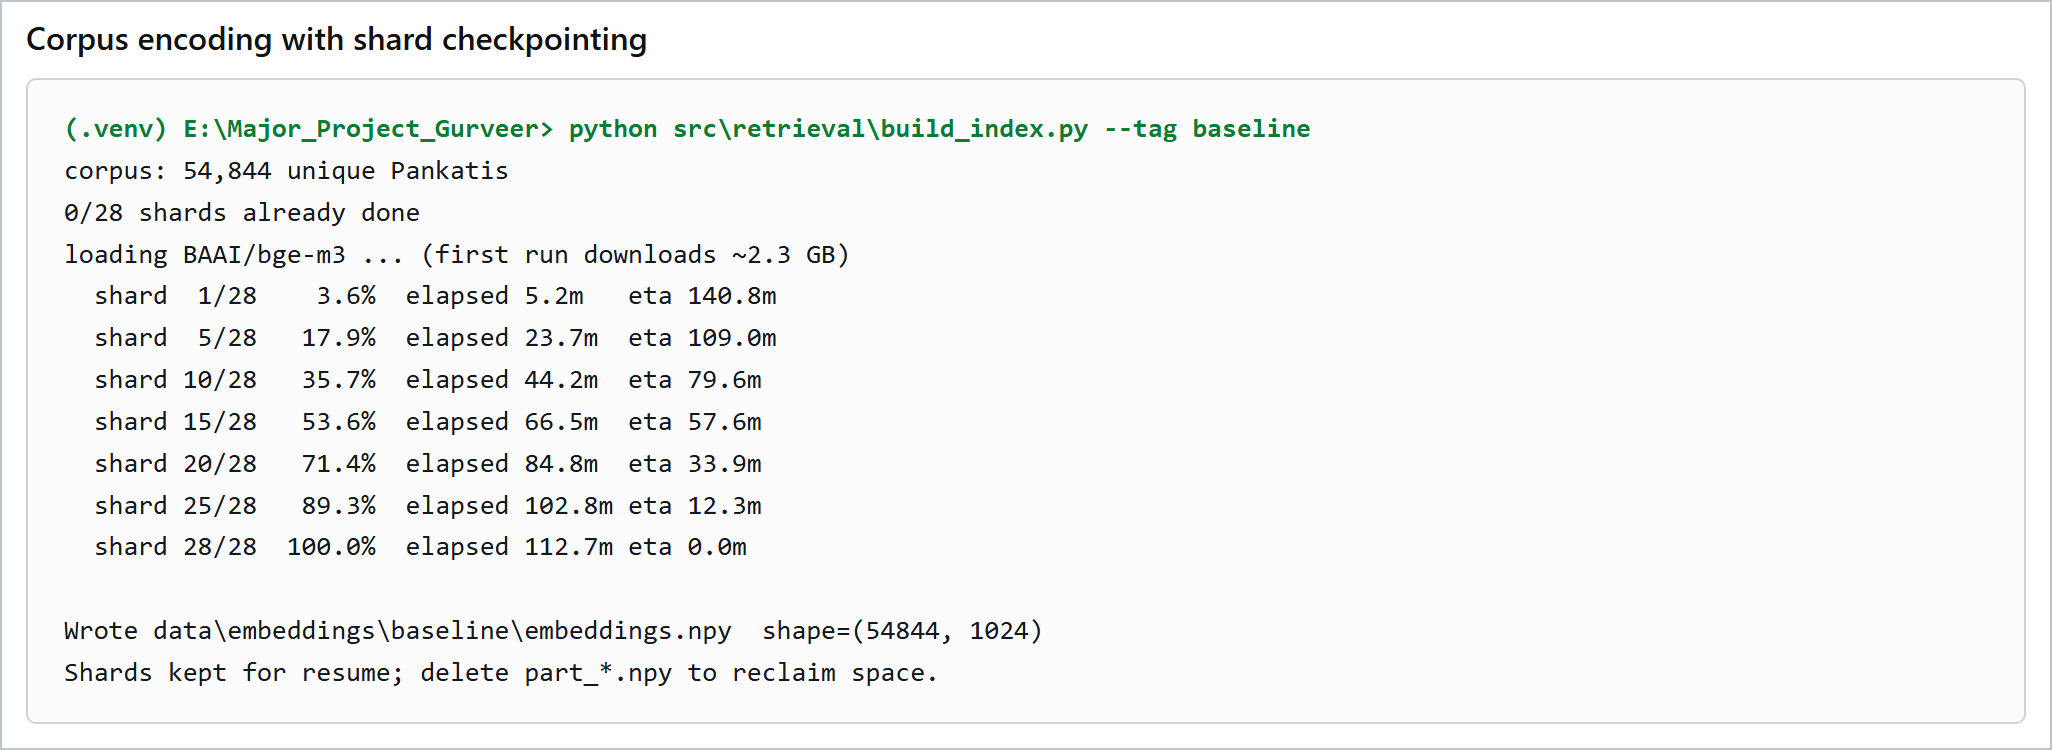
\includegraphics[width=\textwidth]{fig_output_index.png}
\caption{Corpus encoding with shard checkpointing and progress reporting}
\label{fig:auto28}
\end{figure}

% ===================== REFERENCES =====================
\newpage

\addcontentsline{toc}{section}{References}

\bibliographystyle{IEEEtran}
\bibliography{references}

% ===================== END REFERENCES =====================


\end{document}
